%!TEX encoding = UTF-8 Unicode
\documentclass[a4paper]{compendium}
\usepackage[swedish]{babel}

\setlength{\columnsep}{16mm}

\title{
{\bf\Huge\sffamily  Programmering, grundkurs} 
\\ \vspace{2em}
{\sffamily  Lösningar till övningar }
}

%\author{Redaktör: Björn Regnell}
\date{%EDAA45, Lp1-2, HT 2016 \\ 
Datavetenskap, LTH \\ 
Lunds Universitet  \\
\vspace{1em}Kompilerad: \today\\
\vspace{2em}\url{http://cs.lth.se/pgk}
%\url{https://github.com/lunduniversity/introprog}
}

\usepackage{pgffor}  %% http://stackoverflow.com/questions/2561791/iteration-in-latex
                     %  allows:  \foreach \n in {1,...,4}{ do something with \n }

\usepackage{framed}  %  allows:   \begin{framed}\end{framed}
%\newenvironment{Slide}[2][]
%  {\begin{framed}\setlist{noitemsep}\section*{#2}}
%  {\end{framed}}

\usepackage[most]{tcolorbox}
\newenvironment{Slide}[2][]
  {\vspace{0.5em}\begin{tcolorbox}[%breakable, 
                                   enhanced]\setlist{noitemsep}\SlideHeading{#2}}
  {\end{tcolorbox}\vspace{0.5em}}

\newcommand{\Subsection}[1]{} %ignore slide sections
\newcommand{\SlideOnly}[1]{} %ignore slide font size

\newif\ifkompendium  % to allow conditional text in slides only showing up in compendium
\kompendiumtrue      % in slides: \kompendiumfalse
                

%!TEX encoding = UTF-8 Unicode

\newcommand{\ModWeekONE}{Introduktion}
\newcommand{\ExeWeekONE}{expressions}
\newcommand{\LabWeekONE}{kojo}


\newcommand{\ModWeekTWO}{Program, kontrollstrukturer}
\newcommand{\ExeWeekTWO}{programs}
\newcommand{\LabWeekTWO}{--}


\newcommand{\ModWeekTHREE}{Funktioner, abstraktion}
\newcommand{\ExeWeekTHREE}{functions}
\newcommand{\LabWeekTHREE}{irritext}


\newcommand{\ModWeekFOUR}{Objekt, inkapsling}
\newcommand{\ExeWeekFOUR}{objects}
\newcommand{\LabWeekFOUR}{blockmole}


\newcommand{\ModWeekFIVE}{Klasser, datamodellering}
\newcommand{\ExeWeekFIVE}{classes}
\newcommand{\LabWeekFIVE}{--}


\newcommand{\ModWeekSIX}{Mönster, felhantering}
\newcommand{\ExeWeekSIX}{patterns}
\newcommand{\LabWeekSIX}{blockbattle}


\newcommand{\ModWeekSEVEN}{Sekvenser, enumerationer}
\newcommand{\ExeWeekSEVEN}{sequences}
\newcommand{\LabWeekSEVEN}{shuffle}


\newcommand{\ModWeekEIGHT}{Matriser, typparametrar}
\newcommand{\ExeWeekEIGHT}{matrices}
\newcommand{\LabWeekEIGHT}{life}


\newcommand{\ModWeekNINE}{Mängder, tabeller}
\newcommand{\ExeWeekNINE}{lookup}
\newcommand{\LabWeekNINE}{words}


\newcommand{\ModWeekTEN}{Arv, komposition}
\newcommand{\ExeWeekTEN}{inheritance}
\newcommand{\LabWeekTEN}{snake0}


\newcommand{\ModWeekELEVEN}{Kontextuella abstraktioner, api}
\newcommand{\ExeWeekELEVEN}{context}
\newcommand{\LabWeekELEVEN}{snake1}


\newcommand{\ModWeekTWELVE}{Valfri fördjupning, Projekt}
\newcommand{\ExeWeekTWELVE}{extra}
\newcommand{\LabWeekTWELVE}{Projekt0}


\newcommand{\ModWeekTHIRTEEN}{Repetition}
\newcommand{\ExeWeekTHIRTEEN}{examprep}
\newcommand{\LabWeekTHIRTEEN}{Projekt1}


\newcommand{\ModWeekFOURTEEN}{Muntligt prov}
\newcommand{\ExeWeekFOURTEEN}{Munta}
\newcommand{\LabWeekFOURTEEN}{Munta}


\makeatletter
\renewcommand\thechapter{}
\renewcommand\thesection{\@arabic\c@section.}
\renewcommand\thesubsection{\@arabic\c@section.\@arabic\c@subsection}
\makeatother

\setcounter{tocdepth}{1}

\newif\ifPreSolution  % to allow tasks and solutions in same file
\PreSolutionfalse      % in non-solutions: \PreSolutiontrue

\let\QUESTBEGIN\ifPreSolution  % to mark formatting and numbering of exercises
\let\SOLUTION\else  % to mark solutions in the same file as questions
\let\QUESTEND\fi    % to mark end of exercise



\begin{document}
\maketitle
\mainmatter
\tableofcontents

\ExerciseSolution{\ExeWeekONE}
\PreSolutionfalse %!TEX encoding = UTF-8 Unicode
%!TEX root = ../exercises.tex

\ifPreSolution
\Exercise{\ExeWeekONE}\label{exe:W01}

\begin{Goals}
%!TEX encoding = UTF-8 Unicode

\item Förstå vad som händer när satser exekveras och uttryck evalueras.
\item Förstå sekvens, alternativ och repetition.
\item Känna till literalerna för enkla värden, deras typer och omfång.
\item Kunna deklarera och använda variabler och tilldelning, samt kunna rita bilder av minnessituationen då variablers värden förändras.
\item Förstå skillnaden mellan olika numeriska typer, kunna omvandla mellan dessa och vara medveten om noggrannhetsproblem som kan uppstå.
\item Förstå booleska uttryck och värdena \code{true} och \code{false}, samt kunna förenkla booleska uttryck.
\item Förstå skillnaden mellan heltalsdivision och flyttalsdivision, samt användning av rest vid heltalsdivision.
\item Förstå precedensregler och användning av parenteser i uttryck.
\item Kunna använda \code{if}-satser och \code{if}-uttryck.
\item Kunna använda \code{for}-satser och \code{while}-satser.
\item Kunna använda \code{math.random()} för att generera slumptal i olika intervaller.
\item Kunna beskriva skillnader och likheter mellan en procedur och en funktion.

\end{Goals}

\begin{Preparations}
\item \StudyTheory{01}
\item Du behöver en dator med Scala och Kojo installerad, se appendix~\ref{appendix:compile} och  \ref{appendix:kojo}.
\end{Preparations}

\else

\ExerciseSolution{\ExeWeekONE}

\fi  %%% END \ifPreSolution


\BasicTasks




\WHAT{Para ihop begrepp med beskrivning.}

\QUESTBEGIN

\Task \what

\vspace{1em}\noindent Koppla varje begrepp med den (förenklade) beskrivning som passar bäst:

\begin{ConceptConnections}
  litteral & 1 & & A & kan inträffa medan programmet kör \\ 
  sträng & 2 & & B & att översätta kod till exekverbar form \\ 
  sats & 3 & & C & vid anrop beräknas ett returvärde \\ 
  uttryck & 4 & & D & decimaltal med begränsad noggrannhet \\ 
  funktion & 5 & & E & bra då antalet repetitioner är bestämt i förväg \\ 
  procedur & 6 & & F & en kodrad som gör något; kan särskiljas med semikolon \\ 
  exekveringsfel & 7 & & G & beskriver vad data kan användas till \\ 
  kompileringsfel & 8 & & H & antingen sann eller falsk \\ 
  abstrahera & 9 & & I & för att ändra en variabels värde \\ 
  kompilera & 10 & & J & kombinerar värden och funktioner till ett nytt värde \\ 
  typ & 11 & & K & en sekvens av tecken \\ 
  for-sats & 12 & & L & att införa nya begrepp som förenklar kodningen \\ 
  while-sats & 13 & & M & anger ett specifikt datavärde \\ 
  tilldelning & 14 & & N & kan inträffa innan exekveringen startat \\ 
  flyttal & 15 & & O & bra då antalet repetitioner ej är bestämt i förväg \\ 
  boolesk & 16 & & P & vid anrop sker (sido)effekt; returvärdet är tomt \\ 
\end{ConceptConnections}

\SOLUTION

\TaskSolved \what

\begin{ConceptConnections}
  litteral & 1 & ~~\Large$\leadsto$~~ &  D & anger ett specifikt datavärde \\ 
  sträng & 2 & ~~\Large$\leadsto$~~ &  G & en sekvens av tecken \\ 
  sats & 3 & ~~\Large$\leadsto$~~ &  F & en kodrad som gör något; kan särskiljas med semikolon \\ 
  uttryck & 4 & ~~\Large$\leadsto$~~ &  H & kombinerar värden och funktioner till ett nytt värde \\ 
  funktion & 5 & ~~\Large$\leadsto$~~ &  K & vid anrop beräknas ett returvärde \\ 
  procedur & 6 & ~~\Large$\leadsto$~~ &  J & vid anrop sker (sido)effekt; returvärdet är tomt \\ 
  exekveringsfel & 7 & ~~\Large$\leadsto$~~ &  N & kan inträffa medan programmet kör \\ 
  kompileringsfel & 8 & ~~\Large$\leadsto$~~ &  M & kan inträffa innan exekveringen startat \\ 
  abstrahera & 9 & ~~\Large$\leadsto$~~ &  A & att införa nya begrepp som förenklar kodningen \\ 
  kompilera & 10 & ~~\Large$\leadsto$~~ &  C & att översätta kod till exekverbar form \\ 
  typ & 11 & ~~\Large$\leadsto$~~ &  I & beskriver vad data kan användas till \\ 
  for-sats & 12 & ~~\Large$\leadsto$~~ &  O & bra då antalet repetitioner är bestämt i förväg \\ 
  while-sats & 13 & ~~\Large$\leadsto$~~ &  P & bra då antalet repetitioner ej är bestämt i förväg \\ 
  tilldelning & 14 & ~~\Large$\leadsto$~~ &  L & för att ändra en variabels värde \\ 
  flyttal & 15 & ~~\Large$\leadsto$~~ &  E & decimaltal med begränsad noggrannhet \\ 
  boolesk & 16 & ~~\Large$\leadsto$~~ &  B & antingen sann eller falsk \\ 
\end{ConceptConnections}

\QUESTEND






\WHAT{Utskrift i Scala REPL.}

\QUESTBEGIN

\Task \what

\vspace{1em}\noindent Starta Scala REPL \Eng{Read-Evaluate-Print-Loop}.

\begin{REPLnonum}
> scala
Welcome to Scala 3.0.1 (OpenJDK 64-Bit Server VM, Java 11.0.8).
Type in expressions for evaluation. Or try :help.
scala -version.
scala>
\end{REPLnonum}

\Subtask Skriv efter prompten \code{scala>} en sats som skriver ut en valfri (bruklig/knasig) hälsningsfras, genom anrop av proceduren \code{println} med något strängargument. Tryck på \textit{Enter} så att satsen kompileras och exekveras.

\Subtask Skriv samma sats igen (eller tryck pil-upp) men ''glöm bort'' att skriva högerparentesen efter argumentet innan du trycker på \textit{Enter}. Vad händer?

\begin{framed}
\noindent\emph{Tips inför fortsättningen:} Det finns många användbara kortkommandon och andra trix för att jobba snabbt i REPL. Be gärna någon som kan dessa trix att visa dig hur man kan jobba snabbare. Läs appendix \ref{appendix:compile:REPL} och prova sedan att kopiera och klistra in text. Använd piltangenterna för att bläddra i historiken, Ctrl+A för att komma till början av raden, Ctrl+K för att radera resten av raden, etc.
\end{framed}



\SOLUTION
\TaskSolved \what

\SubtaskSolved Till exempel:
\begin{REPLnonum}
scala> println("hejsan svejsan")
\end{REPLnonum}

\SubtaskSolved Om högerparentes fattas får man fortsätta skriva på nästa rad. Detta indikeras med vertikalstreck i början av varje ny rad:
\begin{REPLnonum}
scala> println("hejsan svejsan"
     | + "!"
     | )
hejsan svejsan!
\end{REPLnonum}

\QUESTEND



\WHAT{Konkatenering av strängar.}

\QUESTBEGIN

\Task \what

\Subtask Skriv ett uttryck som konkatenerar två strängar, t.ex. \code{"gurk"} och \code{"burk"}, med hjälp av operatorn \code{+} och studera resultatet. Vad har uttrycket för värde och typ? Vilken siffra står efter ordet \code{res} i variabeln som lagrar resultatet?

\Subtask Använd resultatet från konkateneringen, t.ex. \code{res0} (byt ev. ut \code{0}:an mot siffran efter \code{res} i utskriften från förra evalueringen), och skriv ett uttryck med hjälp av operatorn \code{*} som upprepar resultatet från förra deluppgiften 42 gånger.


\SOLUTION

\TaskSolved \what

\SubtaskSolved
\begin{REPLnonum}
scala> "gurk" + "burk"
res1: String = gurkburk
\end{REPLnonum}
värde: \code{"gurkburk"}, typ:  \code{String}

\SubtaskSolved
\begin{REPLnonum}
scala> res1 * 42
res2: String = gurkatomatgurkatomatgurkatomatgurkatomatgurkatomatgurkatomatgurkatomatgurkatomatgurkatomatgurkatomatgurkatomatgurkatomatgurkatomatgurkatomatgurkatomatgurkatomatgurkatomatgurkatomatgurkatomatgurkatomatgurkatomatgurkatomatgurkatomatgurkatomatgurkatomatgurkatomatgurkatomatgurkatomatgurkatomatgurkatomatgurkatomatgurkatomatgurkatomatgurkatomatgurkatomatgurkatomatgurkatomatgurkatomatgurkatomatgurkatomatgurkatomatgurkatomat
\end{REPLnonum}

\QUESTEND




\WHAT{När upptäcks felet?}

\QUESTBEGIN

\Task \what

\Subtask Vad har uttrycket \code{ "hej" * 3 } för typ och värde? Testa i REPL.

\Subtask Byt ut 3:an ovan mot ett så pass stort heltal så att minnet blir fullt. Hur börjar felmeddelandet? Är detta ett körtidsfel eller ett kompileringsfel?

\Subtask Välj ett värde på argumentet efter operatorn \code{*} så att ett typfel genereras. Hur börjar felmeddelandet? Är detta ett körtidsfel eller ett kompileringsfel?

\begin{framed}
\noindent\emph{Tips inför fortsättningen:} Gör gärna fel när du kodar så lär du dig mer! Träna på att tolka olika felmeddelanden och fråga någon om hjälp om du inte förstår. Kompilatorns utskrifter kan vara till stor hjälp, men är ibland kryptiska. Om du kör fast och inte kommer vidare själv så be om hjälp, \emph{men be om tips snarare än färdiga lösningar} så att du behåller initiativet själv och tar kontroll över nästa steg i ditt lärande.
\end{framed}


\SOLUTION

\TaskSolved \what

\SubtaskSolved Typ: \code{String}, värde: \code{"hejhejhej"}

\SubtaskSolved Körtiddsfel:
\begin{REPLnonum}
scala> "hej" * Int.MaxValue
java.lang.OutOfMemoryError: Java heap space
\end{REPLnonum}

\SubtaskSolved Kompileringsfel: (indikeras av texten \code{<console> ... error:})
\begin{REPLnonum}
scala> "hej" * true
<console>:12: error: type mismatch;
 found   : Boolean(true)
 required: Int
       "hej" * true
\end{REPLnonum}
Ett typfel innebär att kompilatorn inte kan få typerna att överensstämma i t.ex. ett funktionsanrop. I Scala får vi reda på typfel redan vid kompilering medan i andra språk (t.ex. Javascript) upptäcks sådana fel under exekveringen, i värsta fall genom svårhittade buggar som kanske först märks långt senare.

\QUESTEND




\WHAT{Litteraler och typer.}

\QUESTBEGIN

\Task \what

\Subtask Ta hjälp av REPL-kommadot \verb+:type+ (kan förkortas \code{:t}) vid behov för att para ihop nedan litteraler med rätt typ.

\begin{ConceptConnections}[0.35\textwidth]
  \code|1    | & 1 & & A & \code|Float  | \\ 
  \code|1L   | & 2 & & B & \code|Double | \\ 
  \code|1.0  | & 3 & & C & \code|Unit   | \\ 
  \code|1D   | & 4 & & D & \code|Int    | \\ 
  \code|1F   | & 5 & & E & \code|Boolean| \\ 
  \code|'1'  | & 6 & & F & \code|Long   | \\ 
  \code|"1"| & 7 & & G & \code|String | \\ 
  \code|true | & 8 & & H & \code|Double | \\ 
  \code|false| & 9 & & I & \code|Char   | \\ 
  \code|()   | & 10 & & J & \code|Boolean| \\ 
%\Connect{\code|1      |}  {\code|Int    |}
%\Connect{\code|1L     |}  {\code|Long   |}
%\Connect{\code|1.0    |}  {\code|Double |}
%\Connect{\code|1D     |}  {\code|Double |}
%\Connect{\code|1F     |}  {\code|Float  |}
%\Connect{\code|'1'    |}  {\code|Char   |}
%\Connect{\code|\"1\"  |}  {\code|String |}
%\Connect{\code|true   |}  {\code|Boolean|}
%\Connect{\code|false  |}  {\code|Boolean|}
%\Connect{\code|()     |}  {\code|Unit   |}
\end{ConceptConnections}

\Subtask Vad händer om du adderar 1 till det största möjliga värdet av typen \code{Int}?
\\\emph{Tips:} se snabbreferensen \footnote{\url{http://cs.lth.se/pgk/quickref/}} under rubriken ''The Scala type system'' avsnitt ''Methods on numbers''.

\Subtask Vad är skillnaden mellan typerna \code{Long} och \code{Int}?

\Subtask Vad är skillnaden mellan typerna \code{Double} och \code{Float}?


\SOLUTION

\TaskSolved \what

\SubtaskSolved

\begin{ConceptConnections}
  \code|1    | & 1 & ~~\Large$\leadsto$~~ &  C & \code|Int    | \\ 
  \code|1L   | & 2 & ~~\Large$\leadsto$~~ &  F & \code|Long   | \\ 
  \code|1.0  | & 3 & ~~\Large$\leadsto$~~ &  J & \code|Double | \\ 
  \code|1D   | & 4 & ~~\Large$\leadsto$~~ &  D & \code|Double | \\ 
  \code|1F   | & 5 & ~~\Large$\leadsto$~~ &  B & \code|Float  | \\ 
  \code|'1'  | & 6 & ~~\Large$\leadsto$~~ &  A & \code|Char   | \\ 
  \code|"1"| & 7 & ~~\Large$\leadsto$~~ &  E & \code|String | \\ 
  \code|true | & 8 & ~~\Large$\leadsto$~~ &  G & \code|Boolean| \\ 
  \code|false| & 9 & ~~\Large$\leadsto$~~ &  I & \code|Boolean| \\ 
  \code|()   | & 10 & ~~\Large$\leadsto$~~ &  H & \code|Unit   | \\ 
%\ConnectSolved{\code|1      |}  {\code|Int    |}
%\ConnectSolved{\code|1L     |}  {\code|Long   |}
%\ConnectSolved{\code|1.0    |}  {\code|Double |}
%\ConnectSolved{\code|1D     |}  {\code|Double |}
%\ConnectSolved{\code|1F     |}  {\code|Float  |}
%\ConnectSolved{\code|'1'    |}  {\code|Char   |}
%\ConnectSolved{\code|\"1\"  |}  {\code|String |}
%\ConnectSolved{\code|true   |}  {\code|Boolean|}
%\ConnectSolved{\code|false  |}  {\code|Boolean|}
\end{ConceptConnections}

\SubtaskSolved Värdet går över gränsen för vad som får plats i ett 32 bitars heltal och ''börjar om'' på det minsta möjliga heltalet \code{Int.MinValue} eftersom det är så binär aritmetik aritmetik med begränsat antal bitar fungerar i CPU:n.
\begin{REPL}
scala> Int.MaxValue + 1
res3: Int = -2147483648

scala> Int.MinValue
res4: Int = -2147483648
\end{REPL}

\SubtaskSolved Båda är heltal men \code{Long} kan representera större tal än \code{Int}.

\SubtaskSolved Båda är flyttal men \code{Double} har dubbel precision och kan representera större tal med fler decimaler.



\QUESTEND





\WHAT{Matematiska funktioner. Scaladoc.}

\QUESTBEGIN

\Task \what

\Subtask Antag att du har ett schackbräde med 64 rutor. Tänk dig att du börjar med att lägga ett enda riskorn på första rutan och sedan 
lägger dubbelt så många riskorn i en ny hög för varje efterföljande ruta: 1, 2, 4, 8, ...  etc. När du har gjort detta för alla rutor, 
hur många riskorn har du totalt lagt på schackbrädet?\footnote{\url{https://en.wikipedia.org/wiki/Wheat_and_chessboard_problem}}

\emph{Tips:} Du ska beräkna $2^{64} - 1$. Om du skriver \code{math.} i REPL och trycker TAB får du se inbyggda matematiska funktioner i Scalas standardbibliotek:
\begin{REPLnonum}
scala> math.    // Tryck TAB direkt efter punkten och betrakta listan
\end{REPLnonum}
Använd funktionen \code{math.pow} och lämpliga argument. Om du anger \code{math.pow} eller \code{math.pow()} utan argument får du se funktionshuvudet med 
parameterlistan.

Om du surfar till \url{http://www.scala-lang.org/api/current/} och skriver \code{math} i sökrutan och sedan, efter att du klickat på 
\textbf{\texttt{\small scala.math}}, skriver \textbf{\texttt{\small pow}} i rutan längre ner, så filtreras sidan och du hittar dokumentationen 
av \code{ def pow } som du kan klicka på och läsa mer om.

\Subtask Definiera funktionen \code{omkrets} nedan i REPL. Går det bra att utelämna returtyp-annoteringen? Varför? Finns det anledning att ha den kvar?
\begin{Code}
def omkrets(radie: Double): Double = 2 * math.Pi * radie
\end{Code}

\Subtask Jordens (genomsnittliga) diameter (vid ekvatorn) är ca $12 750$ $km$. Skriv ett uttryck som anropar funktionen \code{omkrets} ovan för att beräkna hur många kilometer per dag man ungefär måste färdas om man vill åka jorden runt på 80 dagar.

\SOLUTION

\TaskSolved \what

\SubtaskSolved Beräkning av $2^{64} - 1$ med \code{math.pow} enligt nedan ger ungefär $1.8 \cdot 10^{19}$
\begin{REPL}
scala> math.pow(2, 64) - 1
res0: Double = 1.8446744073709552E19
\end{REPL}

\SubtaskSolved Ja, returtyp-annoteringen \code{: Double} kan utelämnas.

\begin{itemize}
\item Varför kan returtyp utelämnas?\\Eftersom kompilatorns typhärledning kan härleda returtypen.
\item Varför kan man vilja utelämna den?\\Det blir kortare att skriva utan.
\item Anledningar att ange returtyp:
\begin{itemize}
\item  Med explicit returtyp får du hjälp av kompilatorn att redan under kompileringen kontrollera att uttrycket till höger om likhetstecknet har den typ som förväntas.

\item Genom att du anger returtypen explicit får de som enbart läser metodhuvudet (och inte implementationen)
 tydligt se vad som returneras.
\end{itemize}
\end{itemize}

\SubtaskSolved Ca $500$ $km$.
\begin{REPL}
scala> omkrets(12750 / 2) / 80
res0: Double = 500.6913291658733
\end{REPL}

\QUESTEND




\WHAT{Variabler och tilldelning. Förändringsbar och oföränderlig variabel.}

\QUESTBEGIN

\Task \what~

\Subtask Rita en \emph{ny} bild av datorns minne efter \emph{varje} exekverad rad 1--6 nedan. Varje bild ska visa alla variabler som finns i minnet och deras variabelnamn, typ och värde.

\begin{REPL}[numbers=left, numberstyle=\color{black}\ttfamily\scriptsize\selectfont]
scala> var a = 13
scala> val b = a + 1
scala> var c = (a + b) * 2.0
scala> b = 0
scala> a = 0
scala> c = c + 1
\end{REPL}
Efter första raden ser minnessituationen ut så här:

\MEM{a}{Int}{13}

\Subtask Varför blir det fel på rad 4? Är det ett kompileringsfel eller exekveringsfel? Hur lyder felmeddelandet?

\SOLUTION

\TaskSolved \what

\SubtaskSolved

\begin{tabular}{@{}l l l}
\MEM{{\it Efter rad 1:~~~~} a}{Int}{13}\\
\MEM{{\it Efter rad 2:~~~~} a}{Int}{13} & \MEM{b}{Int}{14}\\
\MEM{{\it Efter rad 3:~~~~} a}{Int}{13} & \MEM{b}{Int}{14} & \MEM{c}{Double}{54.0}\\
\MEM{{\it Efter rad 4:~~~~} a}{Int}{13} & \MEM{b}{Int}{14} & \MEM{c}{Double}{54.0}\\
\MEM{{\it Efter rad 5:~~~~} a}{Int}{0} & \MEM{b}{Int}{14} & \MEM{c}{Double}{54.0}\\
\MEM{{\it Efter rad 6:~~~~} a}{Int}{0} & \MEM{b}{Int}{14} & \MEM{c}{Double}{55.0}\\
\end{tabular}

\SubtaskSolved
Oföränderliga variabler deklareras med nyckelordet \code{val}. Det går inte att tilldela en oföränderlig variabel ett nytt värde; vid försök blir det kompileringsfel som lyder \texttt{\textbf{error: reassignment to val}}. Kompileringsfel känns igen med hjälp av texten \texttt{\textbf{error:}}, så som visas nedan:
\begin{REPLnonum}
scala> b = 0
<console>:12: error: reassignment to val
       b = 0
         ^
\end{REPLnonum}

\QUESTEND


\WHAT{Slumptal med \code{math.random()}.}

\QUESTBEGIN

\Task\label{exercise:expressions:roll} \what

\Subtask Vad ger funktionen \code{math.random()} för resultatvärde? Vilken typ? Vad är största och minsta möjliga värde?
\\\emph{Tips:} Se scaladoc här: \Scaladoc och prova i REPL.

\Subtask Deklarera den parameterlösa funktionen \code{def roll: Int = ???} som ska representera ett tärningskast och ge ett slumpmässigt heltal mellan 1 och 6. Testa funktionen genom att anropa den många gånger. \\\emph{Tips:} Använd \code{math.random()} och multiplicera och addera med lämpliga heltal. Omge beräkningen med parenteser och avsluta med \code{.toInt} för att avkorta decimaler och omvandla typen från \code{Double} till \code{Int}.

\SOLUTION

\TaskSolved \what

\SubtaskSolved Ur dokumentationen:
\begin{Code}
/** Returns a Double value with a positive sign,
 *  greater than or equal to 0.0 and less than 1.0.
 */
def random(): Double
\end{Code}
Dokumentationskommentarer, som börjar med \code{/**} och slutar med \code{*/}, ger oss en beskrivning av hur funktionen fungerar. Efter dokumentationskommentaren kommer funktionshuvudet, som här berättar att funktionen heter \code{random} och alltid kommer att returnera en \code{Double}. (Verktyget \code{scaladoc} kan med hjälp av  dokumentationskommentarerna automatiskt generera webbsajter med speciella  dokumentationssidor och sökfunktioner.)

\SubtaskSolved
\begin{REPL}
scala> def roll: Int = (math.random() * 6 + 1).toInt

scala> roll
res0: Int = 4

scala> roll
res1: Int = 1
\end{REPL}

\QUESTEND




\WHAT{Repetition med \code{for}, \code{foreach} och \code{while}.}

\QUESTBEGIN

\Task \what

\Subtask Så här kan en \code{for}-sats ser ut:
\begin{Code}
for i <- 1 to 10 do print(s"$i, ")
\end{Code}
Använd en \code{for}-sats för att skriva ut resultatet av 100 tärningskast med funktionen \code{roll} från uppgift \ref{exercise:expressions:roll}.

\Subtask Så här kan en \code{foreach}-sats ser ut:
\begin{Code}
(1 to 10).foreach(i => print(s"$i, "))
\end{Code}
Använd en \code{foreach}-sats för att skriva ut resultatet av 100 tärningskast med funktionen \code{roll} från uppgift \ref{exercise:expressions:roll}.

\Subtask Så här kan en \code{while}-sats se ut:
\begin{Code}
var i = 1
while i <= 10 do { print(s"$i, "); i = i + 1 }
\end{Code}
Använd en \code{while}-sats för att skriva ut resultatet av 100 tärningskast med funktionen \code{roll} från uppgift \ref{exercise:expressions:roll}. Vad händer om du glömmer \code{i = i + 1} ?


\SOLUTION

\TaskSolved \what

\SubtaskSolved
\begin{Code}
for i <- 1 to 100 do print(s"$roll, ")
\end{Code}

\SubtaskSolved
\begin{Code}
(1 to 100).foreach(i => print(s"$roll, "))
\end{Code}


\SubtaskSolved
\begin{Code}
var i = 1
while i <= 100 do { print(s"$roll, "); i = i + 1 }
\end{Code}

\begin{Code}
var i = 1
while i <= 100 do
    print(s"$roll, ") 
    i += 1
\end{Code}




\QUESTEND






\WHAT{Alternativ med \code{if}-sats och \code{if}-uttryck.}

\QUESTBEGIN

\Task \what

\Subtask Så här kan en \code{if}-sats se ut (notera dubbla likhetstecken):
\begin{Code}
if roll == 3 then println("TRE") else println("INTE TRE")
\end{Code}
Testa ovan i REPL. Skriv sedan en \code{for}-sats som kastar 100 tärningar och skriver ut strängen \code{"GRATTIS! "} om det blir en sexa, annars en ledsen smiley: \code{":("}

\Subtask Så här kan ett \code{if}-uttryck se ut:
\begin{Code}
if roll < 6 then 0 else 1
\end{Code}
Testa ovan i REPL. Skriv sedan en \code{while}-sats som kastar 100 tärningar och räknar antalet sexor. Skriv ut antalet efter \code{while}-satsen.

\SOLUTION

\TaskSolved \what

\SubtaskSolved
\begin{Code}
for i <- 1 to 100 do 
  if roll == 6 then print("GRATTIS! ") else print(":(")
\end{Code}
eller
\begin{Code}
for (i <- 1 to 100) if (roll == 6) print("GRATTIS! ") else print(":(")
\end{Code}

\SubtaskSolved
\begin{Code}
var i = 1
var n = 0
while i <= 100 do
  if roll == 6 then n = n + 1
  i = i + 1
println("Antalet sexor: " + n)
\end{Code}


\QUESTEND



\WHAT{Sekvens, sats och block.}

\QUESTBEGIN

\Task \what

\Subtask Vad gör dessa satser?
\begin{REPLnonum}
scala> def p = { print("san"); print("!"); println("hej")}
scala> p;p;p;p
\end{REPLnonum}

\Subtask
Använd pil-upp för att få tillbaka raden du skrev med definitionen av proceduren \code{p}. Byt plats på strängarna i utskriftsanropen i proceduren \code{p} så att utskriften blir:
\begin{REPLnonum}
hejsan!
hejsan!
hejsan!
hejsan!
\end{REPLnonum}

\Subtask Hur tolkar kompilatorn klammerparenteser och semikolon? Vad är ett block?

\SOLUTION

\TaskSolved \what

\SubtaskSolved
Satserna skapar denna utskrift:
\begin{REPLnonum}
san!hej
san!hej
san!hej
san!hej
\end{REPLnonum}

\SubtaskSolved
\begin{REPLnonum}
scala> def p = { print("hej"); print("san"); println("!")}
scala> p;p;p;p
\end{REPLnonum}

\SubtaskSolved
\begin{itemize}
\item Klammerparenteser används för att gruppera flera satser. 
Klammerparenteser behövs om man vill definiera en funktion som består av mer än en sats. 
Sedan scala 3 kan man istället använda indentering för att definera en funktion med flera rader och satser.

\item Semikolon särskiljer flera satser. Semikolon behövs om man vill skriva många satser på samma rad.


\end{itemize}

\QUESTEND




\WHAT{Heltalsdivision.}

\QUESTBEGIN

\Task \what~Vilket värde och vilken typ hör till vilket uttryck?  Är du osäker på svaret, testa i REPL.

\begin{ConceptConnections}[0.3\textwidth]
  \code| 4 / 42      | & 1 & & A & \code|    4: Int      | \\ 
  \code| 42.0 / 2    | & 2 & & B & \code|   10: Int      | \\ 
  \code| 42 / 4      | & 3 & & C & \code| 21.0: Double   | \\ 
  \code| 42 % 4      | & 4 & & D & \code|true : Boolean  | \\ 
  \code| 4 % 42      | & 5 & & E & \code|false: Boolean  | \\ 
  \code| 40 % 4 == 0 | & 6 & & F & \code|    0: Int      | \\ 
  \code| 42 % 4 == 0 | & 7 & & G & \code|    2: Int      | \\ 
\end{ConceptConnections}

\SOLUTION

\TaskSolved \what

\begin{ConceptConnections}[0.3\textwidth]
  \code| 4 / 42      | & 1 & ~~\Large$\leadsto$~~ &  D & \code|    0: Int      | \\ 
  \code| 42.0 / 2    | & 2 & ~~\Large$\leadsto$~~ &  A & \code| 10.5: Double   | \\ 
  \code| 42 / 4      | & 3 & ~~\Large$\leadsto$~~ &  C & \code|   10: Int      | \\ 
  \code| 42 % 4      | & 4 & ~~\Large$\leadsto$~~ &  E & \code|    2: Int      | \\ 
  \code| 4 % 42      | & 5 & ~~\Large$\leadsto$~~ &  B & \code|    4: Int      | \\ 
  \code| 40 % 4 == 0 | & 6 & ~~\Large$\leadsto$~~ &  G & \code|true : Boolean  | \\ 
  \code| 42 % 4 == 0 | & 7 & ~~\Large$\leadsto$~~ &  F & \code|false: Boolean  | \\ 
\end{ConceptConnections}

\QUESTEND





\WHAT{Booleska värden.}

\QUESTBEGIN

\Task \what~Vilket värde har dessa uttryck?  % Uppgift 13

\Subtask \code{true && true}

\Subtask \code{false && true}

\Subtask \code{true || true}

\Subtask \code{false || true}


\Subtask \code{false || false}

\Subtask \code{true == true}

\Subtask \code{true != false}


\Subtask \code{true > false}

\Subtask \code{true && (1 / 0 > 1)}

\Subtask \code{false && (1 / 0 > 1)}

\SOLUTION

\TaskSolved \what

\SubtaskSolved \code{true}

\SubtaskSolved \code{false}

\SubtaskSolved \code{true}

\SubtaskSolved \code{true}


\SubtaskSolved \code{false}

\SubtaskSolved \code{true}

\SubtaskSolved \code{true}


\SubtaskSolved \code{true}

\SubtaskSolved Undantag kastas: \code{java.lang.ArithmeticException: / by zero}

\SubtaskSolved \code{false}

\QUESTEND





\WHAT{Booleska variabler.}

\QUESTBEGIN

\Task \what~Vad skrivs ut på rad 2 och 4 nedan?

\begin{REPL}
scala> var monster = false
scala> if monster then println("akta dig!!!")
scala> monster = true
scala> if monster then println("akta dig!!!")
\end{REPL}

\SOLUTION

\TaskSolved \what

\begin{itemize}
\item[2:] Ingenting skrivs ut.
\item[4:] \code{akta dig!!!}
\end{itemize}


\QUESTEND






\WHAT{Turtle graphics med Kojo.}

\QUESTBEGIN

\Task \what~På veckans laboration ska du använda Kojo för att verifiera att du kan använda sekvens, alternativ, repetition och abstraktion. Med Kojo ska du skapa Scala-program som ritar färgglada figurer med hjälp av ett lättanvänt Scala-bibliotek för \emph{turtle graphics}\footnote{\url{https://en.wikipedia.org/wiki/Turtle_graphics}}.

Starta Kojo (se appendix \ref{appendix:kojo}). Om du inte redan har svenska menyer: välj svenska i språkmenyn och starta om Kojo.  Skriv in nedan program och tryck på den \emph{gröna} play-knappen. Notera kopplingen mellan satssekvensen och vad som händer i ritfönstret.

\begin{Code}
sudda

fram; höger
fram; vänster
färg(grön)
fram
\end{Code}
\noindent


\Subtask Vad händer om du \emph{inte} börjar programmet med \code{sudda} och kör samma program upprepade gånger? Varför är det bra att börja programmet med \code{sudda}?

\Subtask Skriv kod som ritar en kvadrat enligt bilden nedan.
\vspace{1em}\\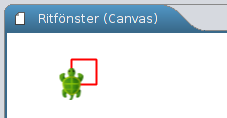
\includegraphics[width=0.47\textwidth]{../img/kojo/kvadrat}

\noindent Prova gärna olika sätt att skriva din kod \emph{utan} att resultatet ändras: skriv satser i sekvens på flera rader eller satser i sekvens på samma rad med semikolon emellan; använd blanktecken och blanka rader i koden. Hur vill du gruppera dina satser så att de är lätta för en människa att läsa?
%Prova att ändra på \emph{ordningen} mellan satserna och studera hur resultatet påverkas. Använd den \emph{gula} play-knappen  (programspårning) för att studera exekveringen i detalj. Vad händer du klickar på satser i ditt program och på rutor i programspårningen?


\Subtask Rita en trappa enligt bilden nedan.


\includegraphics[width=0.3\textwidth]{../img/kojo/stairs}

\Subtask Rita valfri bild på valfri bakgrund med hjälp av några av procedurerna i tabellen nedan. Du kan till exempel rita en rosa triangel med lila konturer mot svart bakgrund. % \ref{lab:kojo:kojo-procedures}.
Försök att underlätta läsbarheten av din kod med hjälp av lämpliga radbrytningar och gruppering av satser.


\begin{table}[H]
\begin{longtable}{l l}\small
\code|fram(100)| & Paddan går framåt 100 steg (25 om argument saknas).\\
\code|färg(rosa)| & Sätter pennans färg till rosa. \\
\code|fyll(lila)| & Sätter ifyllnadsfärgen till lila. \\
\code|fyll(genomskinlig)| & Gör så att paddan \emph{inte} fyller i något när den ritar. \\
\code|bredd(20)| & Gör så att pennan får bredden 20. \\
\code|bakgrund(svart)| & Bakgrundsfärgen blir svart. \\
\code|bakgrund2(grön,gul)| & Bakgrund med övergång från grönt till gult. \\
\code|pennaNer|  & Sätter ner paddans penna så att den ritar när den går. \\
\code|pennaUpp|  & Sänker paddans penna så att den \emph{inte} ritar när den går. \\
\code|höger(45)|   & Paddan vrider sig 45 grader åt höger. \\
\code|vänster(45)| & Paddan vrider sig 45 grader åt vänster. \\
\code|hoppa|       & Paddan hoppar 25 steg utan att rita. \\
\code|hoppa(100)|  & Paddan hoppar 100 steg utan att rita. \\
\code|hoppaTill(100, 200)| & Paddan hoppar till läget (100, 200) utan att rita. \\
\code|gåTill(100, 200)|    & Paddan vrider sig och går till läget (100, 200). \\
\code|öster|   & Paddan vrider sig så att nosen pekar åt höger. \\
\code|väster|  & Paddan vrider sig så att nosen pekar åt vänster. \\
\code|norr|    & Paddan vrider sig så att nosen pekar uppåt. \\
\code|söder|   & Paddan vrider sig så att nosen pekar neråt. \\
\code|mot(100,200)|   & Paddan vrider sig så att nosen pekar mot läget (100, 200) \\
\code|sättVinkel(90)| & Paddan vrider nosen till vinkeln 90 grader. \\
\end{longtable}
%\label{lab:kojo:kojo-procedures}
%\caption{Några användbara procedurer i Kojo.}
\end{table}

\begin{framed}
\noindent\emph{Tips inför fortsättningen:} Ha gärna både REPL och Kojo igång samtidigt. Då kan du undersöka hur olika kodkonstruktioner fungerar i REPL, medan du stegvis skapar allt större program i editorn i Kojo. Detta sätt att jobba har du nytta av under resten av kursen, både om du använder en texteditor och kompilerar i terminalen, och om du använder en professionell integrerad utvecklingsmiljö. Oavsett vilka andra verktyg du kör är det användbart att ha REPL igång i ett eget fönster som hjälp i den kreativa processen, medan du jagar buggar och medan du lär dig nya koncept. Så fort du undrar hur något fungerar i Scala: fram med REPL och testa!
\end{framed}


\SOLUTION

\TaskSolved \what

\SubtaskSolved Genom att börja din Kojo-program med \code{sudda} så startar du exekveringen i samma utgångsläge: en tom rityta \Eng{canvas} där paddan pekar uppåt, pennan är nere och pennans färg är röd.  Då blir det lättare att resonera om vad programmet gör från början till slut, jämfört med om exekveringen beror på resultatet av tidigare exekveringar.


\SubtaskSolved
\begin{Code}
sudda

fram; vänster
fram; vänster
fram; vänster
fram; vänster
\end{Code}


\SubtaskSolved
\begin{Code}
sudda

fram; vänster
fram; höger

fram; vänster
fram; höger

fram; vänster
fram; höger

fram; vänster
\end{Code}


\QUESTEND









\clearpage

\ExtraTasks %%%%%%%%%%%%%%%%%% EXTRAUPPGIFTER



\WHAT{Typ och värde.}

\QUESTBEGIN

\Task \what~Vilket värde och vilken typ hör till vilket uttryck?  Är du osäker på svaret, testa i REPL.

\begin{ConceptConnections}[0.3\textwidth]
  \code|1.0 + 18          | & 1 & & A & \code|42.0: Double    | \\ 
  \code|(41 + 1).toDouble | & 2 & & B & \code|65: Int         | \\ 
  \code|1.042e42 + 1      | & 3 & & C & \code|19.0: Double    | \\ 
  \code|12E6.toLong       | & 4 & & D & \code|12000000: Long  | \\ 
  \code|32.toChar.toString| & 5 & & E & \code|'*': Char       | \\ 
  \code|'A'.toInt         | & 6 & & F & \code|48: Int         | \\ 
  \code|0.toInt           | & 7 & & G & \code|" ": String   | \\ 
  \code|'0'.toInt         | & 8 & & H & \code|1.042E42: Double| \\ 
  \code|'9'.toInt         | & 9 & & I & \code|'q': Char       | \\ 
  \code|'A' + '0'         | & 10 & & J & \code|113: Int        | \\ 
  \code|('A' + '0').toChar| & 11 & & K & \code|0: Int          | \\ 
  \code|"*!%#".charAt(0)| & 12 & & L & \code|57: Int         | \\ 
\end{ConceptConnections}

\SOLUTION

\TaskSolved \what

\begin{ConceptConnections}
  \code|1.0 + 18          | & 1 & ~~\Large$\leadsto$~~ &  E & \code|19.0: Double    | \\ 
  \code|(41 + 1).toDouble | & 2 & ~~\Large$\leadsto$~~ &  L & \code|42.0: Double    | \\ 
  \code|1.042e42 + 1      | & 3 & ~~\Large$\leadsto$~~ &  A & \code|1.042E42: Double| \\ 
  \code|12E6.toLong       | & 4 & ~~\Large$\leadsto$~~ &  K & \code|12000000: Long  | \\ 
  \code|32.toChar.toString| & 5 & ~~\Large$\leadsto$~~ &  G & \code|" ": String   | \\ 
  \code|'A'.toInt         | & 6 & ~~\Large$\leadsto$~~ &  H & \code|65: Int         | \\ 
  \code|0.toInt           | & 7 & ~~\Large$\leadsto$~~ &  I & \code|0: Int          | \\ 
  \code|'0'.toInt         | & 8 & ~~\Large$\leadsto$~~ &  F & \code|48: Int         | \\ 
  \code|'9'.toInt         | & 9 & ~~\Large$\leadsto$~~ &  D & \code|57: Int         | \\ 
  \code|'A' + '0'         | & 10 & ~~\Large$\leadsto$~~ &  B & \code|113: Int        | \\ 
  \code|('A' + '0').toChar| & 11 & ~~\Large$\leadsto$~~ &  J & \code|'q': Char       | \\ 
  \code|"*!%#".charAt(0)| & 12 & ~~\Large$\leadsto$~~ &  C & \code|'*': Char       | \\ 
\end{ConceptConnections}

%\Subtask \code{1.0 + 18}
%
%\Subtask \code{(41 + 1).toDouble}
%
%\Subtask \code{1.042e42 + 1}
%
%\Subtask \code{12E6.toLong}
%
%\Subtask \code{"gurk" + 'a'}
%
%\Subtask \code{32.toChar.toString}
%
%\Subtask \code{'A'.toInt}
%
%\Subtask \linebreak[0] \code{'0'.toInt}
%
%\Subtask \code{'0'.toInt}
%
%\Subtask \code{'9'.toInt}
%
%\Subtask \code{'A' + '0'}
%
%\Subtask \code{('A' + '0').toChar}
%
%\Subtask \code{"*!%#".charAt(0)}
%%%%%%%%%%%%%%%%%%%%%%%%%%%%%%%%%%%%%%%%%%%%%%%%
%\SubtaskSolved \code{Double, 19}
%
%\SubtaskSolved \code{Double, 42}
%
%\SubtaskSolved \code{Double, 1.042E42}
%
%\SubtaskSolved \code{Long, 12000000}
%
%\SubtaskSolved \code{String, gurka}
%
%\SubtaskSolved \code{String, " "}
%
%\SubtaskSolved \code{Int, 65}
%
%\SubtaskSolved \code{Int, 48}
%
%\SubtaskSolved \code{Int,49}
%
%\SubtaskSolved \code{Int,57}
%
%\SubtaskSolved \code{Int, 113}
%
%\SubtaskSolved \code{Char, 'q'}
%
%\SubtaskSolved \code{Char, '*'}


\QUESTEND




\WHAT{Satser och uttryck.}

\QUESTBEGIN

\Task \what

\Subtask Vad är det för skillnad på en sats och ett uttryck?

\Subtask Ge exempel på satser som inte är uttryck?

\Subtask Förklara vad som händer för varje evaluerad rad:
\begin{REPL}
scala> def värdeSaknas = ()
scala> värdeSaknas
scala> värdeSaknas.toString
scala> println(värdeSaknas)
scala> println(println("hej"))
\end{REPL}

\Subtask Vilken typ har literalen \code{()}?

\Subtask Vilken returtyp har \code{println}?

\SOLUTION

\TaskSolved \what

\SubtaskSolved  Ett utryck kan evalueras och resulterar då i ett användbart värde. En sats \emph{gör} något (t.ex. skriver ut något), men resulterat inte i något användbart värde.

\SubtaskSolved \code{println()}

\SubtaskSolved

 \code{värdeSaknas} innehåller Unit

 Skriver ut \code{Unit}

 Skriver ut \code{"()"}

 Skriver ut \code{"()"}

 Skriver först ut hej med det innersta anropet och sen \code{()} med det yttre anropet

\SubtaskSolved  \code{Unit}

\SubtaskSolved  \code{Unit}

\QUESTEND



\WHAT{Procedur med parameter.}

\QUESTBEGIN

\Task \what~En procedur är en funktion som orsakar en effekt, till exempel en utskrift eller en variabeltilldelning, men som inte returnerar något intressant resultatvärde.%
\footnote{I Scala är procedurer funktioner som returnerar det \emph{tomma värdet}, vilket skrivs \code{()} och är av typen \code{Unit}. I Java och flera andra språk finns inget tomt värde och man har en specialsyntax för procedurer som använder nyckelordet \code{void}. }

\Subtask Deklarera en förändringsbar variabel \code{highscore} som initieras till 0.

\Subtask Deklarera en procedur \code{updateHighscore} som tar en parameter \code{points} och tilldelar \code{highscore} ett nytt värde om \code{points} är större än \code{highscore} och skriver ut strängen \code{"REKORD!"}. Om inte \code{points} är större än \code{highscore} ska strängen \code{"GE INTE UPP!"} skrivas ut. Testa proceduren i REPL.

\Subtask Gör en ny variant av \code{updateHighscore}, som \emph{inte} är en procedur utan i stället är en funktion som ger en sträng för senare utskrift. Testa funktionen i REPL.

\SOLUTION

\TaskSolved \what

\SubtaskSolved
\begin{Code}
var highscore = 0
\end{Code}

\SubtaskSolved
\begin{Code}
def updateHighscore(points: Int): Unit =
  if points > highscore then
    highscore = points
    println("REKORD!")
  else println("GE INTE UPP!")
\end{Code}

\SubtaskSolved
\begin{Code}
def updateHighscore(points: Int): String =
  if points > highscore then
    highscore = points
    "REKORD!"
  else "GE INTE UPP!"
\end{Code}



\QUESTEND


\WHAT{Flyttalsaritmetik.}

\QUESTBEGIN

\Task \what

\Subtask Vilket är det minsta positiva värdet av typen \code{Double}?

\Subtask Vad är värdet av detta uttryck? Varför blir det så?
\begin{REPL}
scala> Double.MaxValue + Double.MinPositiveValue == Double.MaxValue
\end{REPL}

\SOLUTION

\TaskSolved \what

\SubtaskSolved

\begin{REPL}
scala> Double.MinPositiveValue
res0: Double = 4.9E-324
\end{REPL}

\SubtaskSolved

\begin{REPL}
scala> Double.MaxValue + Double.MinPositiveValue == Double.MaxValue
res2: Boolean = true
\end{REPL}

\QUESTEND



\WHAT{\code{if}\textit{-sats}.}

\QUESTBEGIN

\Task \what~För varje rad nedan, beskriv vad som skrivs ut.  % Uppgift 18
\begin{REPL}
scala> if !true then println("sant") else println("falskt")
scala> if !false then println("sant") else println("falskt")
scala> def singlaSlant = if math.random() < 0.5 then "krona" else "klave"
scala> for i <- 1 to 5 do print(s"$i:$singlaSlant ")
\end{REPL}

\SOLUTION

\TaskSolved \what

\begin{enumerate}
\item Utskrift: \code{falskt}
\item Utskrift: \code{sant}
\item Inget skrivs ut, funktionen deklareras men körs ej.
\item Utskrift: \code{1:krona 2:klave 3:krona 4:krona 5:klave } eller liknande beroende på vilka slumptal \code{math.random()} ger.
\end{enumerate}

\QUESTEND




\WHAT{\code{if}\textit{-uttryck}.}

\QUESTBEGIN

\Task  Deklarera följande variabler med nedan initialvärden:

\begin{REPLnonum}
scala> var grönsak = "gurka"
scala> var frukt = "banan"
\end{REPLnonum}

Ange för varje rad nedan vad uttrycket har för värde och typ:
\begin{REPLnonum}
scala> if grönsak == "tomat" then "gott" else "inte gott"
scala> if frukt == "banan" then "gott" else "inte gott"
scala> if true then grönsak else 42
scala> if false then grönsak else 42
\end{REPLnonum}

\SOLUTION


\TaskSolved \what~Notera typen \code{Any} på de sista två uttrycken.

\begin{REPLnonum}
scala> if grönsak == "tomat" then "gott" else "inte gott"
res0: String = inte gott

scala> if frukt == "banan" then "gott" else "inte gott"
res1: String = gott

scala> if true then grönsak else 42
res2: Any = gurka

scala> if false then grönsak else 42
res3: Any = 42
\end{REPLnonum}


\QUESTEND





\WHAT{Modulo-operatorn {\tt \%} och Booleska värden.}

\QUESTBEGIN

\Task \what

\Subtask Deklarera en funktion \code{def isEven(n: Int): Boolean = ???} som ger \code{true} om talet \code{n} är jämnt, annars \code{false}.

\Subtask Deklarera en funktion \code{def isOdd(n: Int): Boolean = ???} som ger \code{false} om talet \code{n} är jämnt, annars \code{true}.

\SOLUTION


\TaskSolved \what

\SubtaskSolved
\begin{REPL}
scala> def isEven(n: Int): Boolean = n % 2 == 0

scala> isEven(42)
res0: Boolean = true

scala> isEven(43)
res1: Boolean = false

\end{REPL}


\SubtaskSolved
\begin{REPL}
scala> def isOdd(n: Int): Boolean = !isEven(n)

scala> isOdd(42)
res2: Boolean = false

scala> isOdd(43)
res3: Boolean = true
\end{REPL}


\QUESTEND





\WHAT{Skillnader mellan \code{var}, \code{val}, \code{def}.}

\QUESTBEGIN

\Task \what~

\Subtask
 Evaluera varje rad en i taget i tur och ordning i Scala REPL. För varje rad nedan: förklara för vad som händer och notera värde och ev fel. % Uppgift 15
\begin{REPL}
scala> var x = 30
scala> x + 1
scala> x = x + 1
scala> x == x + 1
scala> val y = 20
scala> y = y + 1
scala> var z = { println("hej z!"); math.random() }
scala> def w = { println("hej w!"); math.random() }
scala> z
scala> z
scala> z = z + 1
scala> w
scala> w
scala> w = w + 1
\end{REPL}


\Subtask Vad är det för skillnad på \code{var}, \code{val} och \code{def}?



\SOLUTION

\TaskSolved \what

\SubtaskSolved
\begin{REPL}
  scala> var x = 30
  x: Int = 30

  scala> x + 1
  res6: Int = 31

  scala> x = x + 1
  x: Int = 31

  scala> x == x + 1
  res7: Boolean = false

  scala> val y = 20
  y: Int = 20

  scala> y = y + 1
  <console>:12: error: reassignment to val
         y = y + 1
           ^

  scala> var z = { println("hej z!"); math.random() }
  hej z!
  z: Double = 0.3381365875903367

  scala> def w = { println("hej w!"); math.random() }
  w: Double

  scala> z
  res8: Double = 0.3381365875903367

  scala> z
  res9: Double = 0.3381365875903367

  scala> z = z + 1
  z: Double = 1.3381365875903368

  scala> w
  hej w!
  res10: Double = 0.06420209879434557

  scala> w
  hej w!
  res11: Double = 0.5777951341051852

  scala> w = w + 1
  <console>:12: error: value w_= is not a member of object
         w = w + 1
\end{REPL}


\SubtaskSolved
\begin{itemize}
\item \code{var namn = uttryck} används för att deklarera en förändringsbar variabel. Namnet kan med hjälp av en tilldelningssats referera till nya värden.

\item \code{val namn = uttryck} används för att deklarera en oföränderlig variabel som efter initialisering inte kan förändras med tilldelningssatser. Vid försök ges kompileringsfel.
\item \code{def namn = uttryck} används för att deklarera en funktion vars uttryck evalueras varje gång den anropas.
\end{itemize}

\QUESTEND




\WHAT{Skillnaden mellan \code{if} och \code{while}.}

\QUESTBEGIN

\Task \what~Vad blir resultatet av rad 3 och 4?

\begin{REPL}
scala> def lotto1 = if math.random() > 0.5 then print("vinst :) ")
scala> def lotto2 = while math.random() > 0.5 do print("vinst :) ")
scala> lotto1
scala> lotto2
\end{REPL}

\SOLUTION

\TaskSolved \what

\begin{itemize}
\item Rad 3: Har du tur (50\% chans) får du vinst en gång.

\item Rad 4: Har du tur får du många vinster i rad. Sannolikheten för $n$ vinster i rad är $(\frac{1}{2})^n$.
\end{itemize}
\QUESTEND












\clearpage

\AdvancedTasks   %%%%%%%%%%%%%%%%%%% FÖRDJUPNINGSUPPGIFTER





\WHAT{Logik och De Morgans Lagar.}

\QUESTBEGIN

\Task \what~Förenkla följande uttryck. Antag att \code{poäng} och \code{highscore} är heltalsvariabler medan \code{klar} är av typen \code{Boolean}.
  % Uppgift 24

\Subtask \code{poäng > 100 && poäng > 1000}

\Subtask \code{poäng > 100 || poäng > 1000}

\Subtask \code{!(poäng > highscore)}

\Subtask \code{!(poäng > 0 && poäng < highscore) }

\Subtask \code{!(poäng < 0 || poäng > highscore) }

\Subtask \code{klar == true}

\Subtask \code{klar == false}

\SOLUTION

\TaskSolved \what


\SubtaskSolved \code{poäng > 1000}

\SubtaskSolved \code{poäng > 100}

\SubtaskSolved \code{poäng <= highscore}

\SubtaskSolved \code{poäng <= 0 || poäng >= highscore }

\SubtaskSolved \code{poäng >= 0 && poäng <= highscore}

\SubtaskSolved \code{klar}

\SubtaskSolved \code{!klar}


\QUESTEND






\WHAT{Stränginterpolatorn \code{s}.}

\QUESTBEGIN

\Task \what~Med ett \code{s} framför en strängliteral får man hjälp av kompilatorn att, på ett typsäkert sätt, infoga variabelvärden i en sträng.
Variablernas namn ska föregås med ett dollartecken , t.ex. \code{s"Hej $namn"}.
Om man vill evaluera ett uttryck placeras detta inom klammer direkt efter dollartecknet, t.ex.
\code/s"Dubbla längden: ${namn.size * 2}"/

\Subtask Vad skrivs ut nedan?
\begin{REPL}
scala> val f = "Kim"
scala> val e = "Finkodare"
scala> println(s"Namnet '$f $e' har ${f.size + e.size} bokstäver.")
\end{REPL}

\Subtask Skapa följande utskrifter med hjälp av stränginterpolatorn \code{s} och variablerna \code{f} och \code{e} i föregående deluppgift.
\begin{REPL}
Kim har 3 bokstäver.
Finkodare har 9 bokstäver.
\end{REPL}

\SOLUTION

\TaskSolved \what

\SubtaskSolved
\begin{REPLnonum}
Namnet 'Kim Finkodare' har 12 bokstäver.
\end{REPLnonum}

\SubtaskSolved
\begin{REPLnonum}
println(s"$f har  ${f.size} bokstäver.")
println(s"$e har  ${e.size} bokstäver.")
\end{REPLnonum}

\QUESTEND



\WHAT{Tilldelningsoperatorer.}

\QUESTBEGIN

\Task \what~Man kan förkorta en tilldelningssats som förändrar en variabel, t.ex. \code{x = x + 1}, genom att använda så kallade tilldelningsoperatorer och skriva \code{x += 1} som betyder samma sak. Rita en ny bild av datorns minne efter varje rad nedan. Bilderna ska visa variablers namn, typ och värde.

\begin{REPL}
scala> var a = 40
scala> var b = a + 40
scala> a += 10
scala> b -= 10
scala> a *= 2
scala> b /= 2
\end{REPL}

\SOLUTION

\TaskSolved \what

\begin{tabular}{l l}
\MEM{{\it Efter rad1:~~~~} a}{Int}{40}\\
\MEM{{\it Efter rad2:~~~~} a}{Int}{40} & \MEM{b}{Int}{80}\\
\MEM{{\it Efter rad3:~~~~} a}{Int}{50} & \MEM{b}{Int}{80}\\
\MEM{{\it Efter rad4:~~~~} a}{Int}{50} & \MEM{b}{Int}{70} \\
\MEM{{\it Efter rad5:~~~~} a}{Int}{100} & \MEM{b}{Int}{70} \\
\MEM{{\it Efter rad6:~~~~} a}{Int}{100} & \MEM{b}{Int}{35} \\
\end{tabular}

\QUESTEND






\WHAT{Stora tal.}

\QUESTBEGIN

\Task \what~Om vi vill beräkna $2^{64} -1$ som ett exakt heltal\footnote{\url{https://en.wikipedia.org/wiki/Wheat_and_chessboard_problem}} blir det större än \code{Int.MaxValue}, så vi kan tyvärr inte använda snabba \code{Int}. Till vår räddning: \code{BigInt}

\Subtask Läs om \code{BigInt} och \code{BigDecimal} på \Scaladoc \\ Notera vad de kan användas till.

\Subtask Du skapar ett \code{BigInt}-heltal med \code{BigInt(2)} och kan anropa funktionen \code{pow} på en \code{BigInt} med punktnotation. Beräkna $2^{64} -1$ som ett exakt heltal.

\Subtask Vilka nackdelar finns med \code{BigInt} och \code{BigDecimal}?

\SOLUTION

\TaskSolved \what

\SubtaskSolved \code{BigInt} kan användas i stället för \code{Int} vid mycket stora heltal. Det finns förståss även \code{Long} som har dubbelt omfång jämfört med \code{Int}, medan \code{BigInt} kan ha godtyckligt många siffror (ända tills minnet tar slut) och kan därmed representera ofantligt stora tal. \code{BigDecimal} kan användas i stället för \code{Double} vid mycket stora decimaltal.

\SubtaskSolved
\begin{REPL}
scala> BigInt(2).pow(64)
res0: scala.math.BigInt = 18446744073709551616
\end{REPL}

\SubtaskSolved Beräkningar går mycket långsammare och de är lite krångligare att använda.

\QUESTEND





\WHAT{Precedensregler}

\QUESTBEGIN

\Task \what~Evalueringsordningen kan styras med parenteser. Vilket värde och vilken typ har följande uttryck?

\Subtask \code{23 + 2 * 2 + (23 + 2) * 2}

\Subtask \code{(-(2 - 42)) / (1 + 1 + 1)}

\Subtask \code{(-(2 - 42)) / (-1)/(1 + 1 + 1)}

\SOLUTION

\TaskSolved \what

\SubtaskSolved \code{77:  Int}

\SubtaskSolved \code{13: Int}

\SubtaskSolved \code{-13: Int}

\QUESTEND



\WHAT{Dokumentation av paket i Java och Scala.}

\QUESTBEGIN

\Task \what


\Subtask Genom att trycka på tab tangenten kan man se vad som finns i olika paket. Vad heter konstanten $\pi$  i \code{java.lang.Math} (notera stort M) respektive \code{scala.math.}?

\begin{REPL}
scala> java.lang.Math.    //tryck TAB efter punkten
scala> scala.math.        //tryck TAB efter punkten
\end{REPL}

\Subtask Jämför dokumentationen för klassen \code{java.lang.Math} här: \\ \url{https://docs.oracle.com/javase/8/docs/api/} \\
med dokumentationen för paketet \code{scala.math} här: \\
\url{http://www.scala-lang.org/api} \\
Ge exempel på vad man kan göra på webbsidan med Scala-dokumentationen som man \emph{inte} kan göra i motsvarande webbsida Java-dokumentation.

\Subtask Vad gör metoden \code{hypot}? Vad är det som är bra med att använda \code{hypot} i stället för att själv implementera beräkningen med hjälp av kvadratrot, multiplikation och addition?

\SOLUTION

\TaskSolved \what

\SubtaskSolved Scala: \code{Pi}, Java: \code{PI}

\SubtaskSolved Man kan söka och filtrera fram alla förekomster av en viss teckenkombination.

\SubtaskSolved Räknar ut hypotenusan (Pythagoras sats) utan risk för avrundningsproblem i mellanberäkningar.


\QUESTEND





\WHAT{Noggrannhet och undantag i aritmetiska uttryck.}

\QUESTBEGIN

\Task \what~Vad blir resultatet av uttrycken nedan? Notera undantag \Eng{exceptions} och noggrannhetsproblem.

\Subtask \code{Int.MaxValue + 1}

\Subtask \code{1 / 0}

\Subtask \code{1E8 + 1E-8}

\Subtask \code{1E9 + 1E-9}

\Subtask \code{math.pow(math.hypot(3,6), 2)}

\Subtask\Uberkurs \code{1.0 / 0}

\Subtask\Uberkurs \code{(1.0 / 0).toInt}

\Subtask\Uberkurs \code{math.sqrt(-1)}

\Subtask\Uberkurs \code{math.sqrt(Double.NaN)}

\Subtask \code{throw new Exception("PANG!!!")}

\SOLUTION

\TaskSolved \what

\SubtaskSolved \code{-2147483648} vilket motsvarar \code{Int.MinValue}.

\SubtaskSolved Ett undantag kastas: \code{java.lang.ArithmeticException: / by zero}

\SubtaskSolved \code{1.0000000000000001E8} (som förväntat)

\SubtaskSolved Avrundas till \code{1E9} (flyttalsaritmetik med noggrannhetsproblem: ett stort flyttal plus ett (alltför) litet flyttal kan ge samma tal. Det lilla talet ''försvinner'').


\SubtaskSolved \code{45.00000000000001} (flyttalsaritmetik med noggrannhetsproblem: enligt ''normal'' aritmetik ska det bli exakt 45.)

\SubtaskSolved \code{Infinity} (som även ges av \code{Double.PositiveInfinity} och som representerar den positiva oändligheten).

\SubtaskSolved \code{2147483647} vilket motsvarar \code{Int.MaxValue}.

\SubtaskSolved \code{NaN} vilket betyder ''Not a Number''.

\SubtaskSolved \code{NaN} vilket betyder ''Not a Number''.

\SubtaskSolved Ett undantag kastas: \code{java.lang.Exception: PANG!!!}

\QUESTEND



\WHAT{Modulo-räkning med negativa tal.}

\QUESTBEGIN

\Task\Uberkurs \what~Läs om moduloräkning här: \\
 \href{https://en.wikipedia.org/wiki/Modulo\_operation}{en.wikipedia.org/wiki/Modulo\_operation} \\
 och undersök hur det blir med olika tecken (positivt resp. negativt) på moduloräkning med $dividend \% divisor$ i Scala.


\SOLUTION

\TaskSolved \what~I Scala har resultatet samma tecken som dividenden.
\begin{REPL}
scala> 1 % 2
res0: Int = 1

scala> -1 % 2
res1: Int = -1

scala> -1 % -2
res2: Int = -1

scala> 1 % -2
res3: Int = 1

\end{REPL}

\QUESTEND




\WHAT{Bokstavliga identifierare.}

\QUESTBEGIN

\Task\Uberkurs \what~Läs om identifierare i Scala och speciellt \emph{literal identifiers} här: \url{http://www.artima.com/pins1ed/functional-objects.html#6.10}.

\Subtask Förklara vad som händer nedan:
\begin{REPLnonum}
scala> val `bokstavlig val` = 42
scala> println(`bokstavlig val`)
\end{REPLnonum}

\Subtask Scala och Java har olika uppsättningar med reserverade ord. På vilket sätt kan ''backticks'' vara använbart med anledning av detta?

\SOLUTION

\TaskSolved \what

\SubtaskSolved Variabeln får namnet 'bokstavlig val', bakåt-apostrofer \Eng{backticks} gör att man kan namnge variabler till annars otillåtna namn, t.ex. med mellanrum eller nyckelord i sig.

\SubtaskSolved Backticks i Scala möjliggör alla möjliga tecken i namn. Exempel på användning: I java finns en metod som heter \jcode{java.lang.Thread.yield} men i Scala är yield ett nyckelord; för att komma runt det går det att i Scala skriva \jcode{java.lang.Thread.`yield`}

\QUESTEND












\WHAT{\code{java.lang.Integer}, hexadecimala litteraler, BigDecimal.}

\QUESTBEGIN

\Task\Uberkurs \what~

\Subtask Sök upp dokumentationen för \code{java.lang.Integer}.\\Använd metoderna \code{toBinaryString} och \code{toHexString} för att fylla i tabellen nedan.

\begin{table}[H]
\begin{tabular}{l | l | l}
decimalt heltal & binärt värde & hexadecimalt värde \\
\hline
$33$ &   &  \\
$42$ &   &  \\
$64$ &   &  \\
\end{tabular}
\end{table}

\Subtask Hur anger man det hexadecimala heltalsvärdet 10c (motsvarar 268 decimalt) som en litteral i Scala?

\Subtask Vad blir \code{0x10} upphöjt till $c =$ ljusets hastighet i $m/s$? \emph{Tips:} Använd \code{BigDecimal}.

\SOLUTION

\TaskSolved \what

\SubtaskSolved

\begin{REPL}
scala> import Integer.{toBinaryString => toBin, toHexString => toHex}

scala> for i <- Seq(33, 42, 64) do println(s"$i \t ${toBin(i)} \t ${toHex(i)}")
33 	 100001 	 21
42 	 101010 	 2a
64 	 1000000 	 40
\end{REPL}


\SubtaskSolved Det hexadecimala heltalet $10c$ kan anges med litteralen \code{0x10c} i Scala, Java och många andra språk: \footnote{\url{https://en.wikipedia.org/wiki/0x10c}}
\begin{REPL}
scala> 0x10c
res0: Int = 268
\end{REPL}

\SubtaskSolved \footnote{\url{https://c418.bandcamp.com/album/0x10c}}
\begin{REPL}
scala> val c = 299792458
c: Int = 299792458

scala> BigDecimal(0x10).pow(c)
res68: scala.math.BigDecimal = 2.124892963227906613060986110887672E+360986089
\end{REPL}


\QUESTEND









\WHAT{Strängformatering.}

\QUESTBEGIN

\Task\Uberkurs \what~Läs om \code{f}-interpolatorn här:\\
\url{http://docs.scala-lang.org/overviews/core/string-interpolation.html} \\
Hur kan du använda \code{f}-interpolatorn för att göra följande utskrift i REPL? Ändra rad 3 vid \code{???} så att flyttalet \code{g} avrundas till tre decimaler innan utskrift sker.
\begin{REPL}
scala> val g = 2 / 3.0
scala> val str = f"Jättegurkan är $g??? meter lång"
scala> println(str)
Jättegurkan är 0.667 meter lång
\end{REPL}

\SOLUTION

\TaskSolved \what

\begin{Code}
val str = f"Jättegurkan är $g%1.3f meter lång"
\end{Code}
(Om du tycker att \code{$g%1.3f}
ser kryptiskt ut, så kan du trösta dig med att du nu får chansen att föra vidare ett anrikt arv från det urgamla språket C och den sägenomspunna funktionen \code{printf} till kommande generationer av invigda kodmagiker.)

\QUESTEND




\WHAT{Multiplikationsvarning.}

\QUESTBEGIN

\Task \what~Sök upp dokumentationtionen för\\\code{java.lang.Math.multiplyExact} och läs om vad den metoden gör.

\Subtask Vad händer här?

\begin{REPLnonum}
scala> Math.multiplyExact(1, 2)
scala> Int.MaxValue * 2
scala> Math.multiplyExact(Int.MaxValue, 2)
\end{REPLnonum}

\Subtask Varför kan man vilja använda \code{java.lang.Math.multiplyExact} i stället för ''vanlig'' multiplikation?

\SOLUTION

\TaskSolved \what

\SubtaskSolved Den andra multiplikationen flödar över \Eng{overflow} gränsen för största möjliga värdet av en \code{Int}. I den tredje multiplikationen kastas i stället ett undantag \code{java.lang.ArithmeticException: integer overflow}


\begin{REPLnonum}
scala> Math.multiplyExact(1, 2)
res70: Int = 2

scala> Int.MaxValue * 2
res71: Int = -2

scala> Math.multiplyExact(Int.MaxValue, 2)
java.lang.ArithmeticException: integer overflow
  at java.lang.Math.multiplyExact(Math.java:867)
  ... 42 elided
\end{REPLnonum}

\SubtaskSolved Används då man vill vara helt säker på att overflow-buggar ''smäller'' direkt i stället för att generera felaktiga resultat vars konsekvenser kanske manifesterar sig långt senare. Dock är \code{multiplyExact} aningen långsammare än vanlig multiplikation.


\QUESTEND








\WHAT{Dekorera \code{Int} med extra operatorer.}

\QUESTBEGIN

\Task\Uberkurs \what\footnote{En utmanande överkursuppgift som visar Scalas kraftfullhet. Se fördjupningslänkar i facit.}\\Kim Kodmagiker tycker att \code{Math.multiplyExact} är för krångligt att skriva och utökar därför typen \code{Int} med en extra operator:

\begin{Code}
implicit class IntDecorator(val i: Int) extends AnyVal {
  def *!(j: Int) = Math.multiplyExact(i,j)
}
\end{Code}

\Subtask Klistra in koden ovan i REPL och prova den extra operatorn.

\Subtask Hjälp Kim Kodmagiker att lägga till fler operatorer på värden av typen \code{Int}, som gör att det även går att använda \code{Math.subtractExact} och \code{Math.addExact} smidigt.

\Subtask Testa ett sammansatt uttryck som använder alla extrametoder på \code{Int}. Tycker du det blev mer lättläst eller mer kryptiskt med de nya operatorerna?

\SOLUTION

\TaskSolved \what

\SubtaskSolved

\begin{REPL}
scala> Int.MaxValue *! 1
res0: Int = 2147483647

scala> Int.MaxValue *! 2
java.lang.ArithmeticException: integer overflow
  at java.lang.Math.multiplyExact(Math.java:867)
  at IntExtra.$times$bang(<console>:16)
  ... 32 elided

\end{REPL}

Kort förklaring:
\begin{itemize}
\item \code{implicit class MinDekorator(x: Typ)} gör så att operationer i dekoratorklassen \code{MinDekorator} automatiskt görs tillgängliga på värden av typen \code{Typ}.%
\footnote{Fördjupning: \url{http://docs.scala-lang.org/overviews/core/implicit-classes.html}}

\item \code{extends AnyVal} gör så att kompilatorn försöker generera maskinkod som blir lika effektiv som vid direkt användning av det underliggande värdet.%
\footnote{Fördjupning: \url{http://docs.scala-lang.org/overviews/core/value-classes.html}}
\end{itemize}


\SubtaskSolved

\begin{Code}
implicit class IntDecorator(val i: Int) extends AnyVal{
  def *!(j: Int) = Math.multiplyExact(i,j)
  def +!(j: Int) = Math.addExact(i,j)
  def -!(j: Int) = Math.subtractExact(i,j)
}
\end{Code}


\SubtaskSolved Det blir lätt väldigt kryptiskt med namn som består av flera specialtecken. Om du \emph{verkligen} vill ha sådana operatorer är det \emph{mycket} lämpligt att också erbjuda varianter i klartext:
\begin{Code}
implicit class IntDecorator(val i: Int) extends AnyVal{
  def mulExact(j: Int) = Math.multiplyExact(i,j)
  def *!(j: Int) = i mulExact j

  def addExact(j: Int) = Math.addExact(i,j)
  def +!(j: Int) = i addExact j

  def subExact(j: Int) = Math.subtractExact(i,j)
  def -!(j: Int) = i subExact j
}

\end{Code}


\QUESTEND



%%%%%%%%%%%%%%%%%%%%%%%%%%%%%%%%%%%%%%%%%%%%%%%%
%%%%%%%%%%%%%%%%%%%%%%%%%%%%%%%%%%%%%%%%%%%%%%%%
%%%%%%%%%%%%%%%%%%%%%%%%%%%%%%%%%%%%%%%%%%%%%%%%
%%%%%%%%%%%%%%%%%%%%%%%%%%%%%%%%%%%%%%%%%%%%%%%%
%%%%%%%%%%%%%%%%%%%%%%%%%%%%%%%%%%%%%%%%%%%%%%%%
%%%%%%%%%%%%%%%%%%%%%%%%%%%%%%%%%%%%%%%%%%%%%%%%
%%%%%%%%%%%%%%%%%%%%%%%%%%%%%%%%%%%%%%%%%%%%%%%%
%%%%%%%%%%%%%%%%%%%%%%%%%%%%%%%%%%%%%%%%%%%%%%%%
%%%%%%%%%%%%%%%%%%%%%%%%%%%%%%%%%%%%%%%%%%%%%%%%


%% Saker som inte fick plats:



%\Task Läs om BigInt och BigDecimal här: \href{http://alvinalexander.com/scala/how-to-use-large-integer-decimal-numbers-in-scala-bigint-bigdecimal}{alvinalexander.com/scala/how-to-use-large-integer-decimal-numbers-in-scala-bigint-bigdecimal} och prova att skapa riktigt stora tal med hjälp av metoden \code{pow} på BigInt och tal med riktigt många decimaler med BigDecimal dess metod \code{pow}.


%
%
%\Subtask\Pen Sök med Ctrl+F i webbläsaren och efter förekomster av texten \textit{''overflow''} i javadoc för klassen \code{java.lang.Math} i JDK 8. Vad är ''overflow''? Vilka metoder finns i \code{java.lang.Math} som hjälper dig att upptäcka om det blir overflow?
%
%\Task Använda Scala REPL för att undersöka konstanterna nedan. Vilket av dessa värden är negativt? Vad kan man ha för praktisk nytta av dessa värden i ett program som gör flyttalsberäkningar?
%
%\Subtask \code{java.lang.Double.MIN_VALUE}
%
%\Subtask \code{scala.Double.MinValue}
%
%\Subtask \code{scala.Double.MinPositiveValue}
%
%\Task För typerna \code{Byte}, \code{Short}, \code{Char}, \code{Int}, \code{Long}, \code{Float}, \code{Double}: Undersök hur många bitar som behövs för att representera varje typs omfång? \\*
%\textit{Tips:} Några användbara uttryck: \\*
% \code{Integer.toBinaryString(Int.MaxValue + 1).size} \\*
% \code{Integer.toBinaryString((math.pow(2,16) - 1).toInt).size} \\*
% \code{1 + math.log(Long.MaxValue)/math.log(2)}
%Se även språkspecifikationen för Scala, kapitlet om heltalsliteraler: \\
%\url{http://www.scala-lang.org/files/archive/spec/2.11/01-lexical-syntax.html#integer-literals}
%
%\Subtask Undersök källkoden för paketobjektet \code{scala.math} här: \\
%\url{https://github.com/scala/scala/blob/v2.11.7/src/library/scala/math/package.scala} \\
%Hur många olika överlagrade varianter av funktionen \code{abs} finns det och för vilka parametertyper är den definierad?

\PreSolutionfalse %!TEX encoding = UTF-8 Unicode
%!TEX root = ../solutions.tex

%\ExerciseSolution{\ExeWeekONE}
%\BasicTasks %%%%%%%%%%%
% uppgift 2

\noindent\TODO{HÄREFTER KOMMER GAMLA LÖSNINGAR FRÅN \code{-solutions.tex}}



% uppgift 4 
\Task  
\begin{REPLnonum}
hejsan
42
gurka
\end{REPLnonum}
\begin{itemize}[noitemsep,nolistsep]
\item Klammerparenteser används för att gruppera flera satser. Klammerparenteser behövs om man vill definiera en funktion som består av mer än en sats. 

\item Semikolon avskiljer flera satser. Semikolon behövs om man vill skriva många satser på samma rad.
\end{itemize}
\Task % uppgift 5

\Subtask  Ett utryck kan evalueras och resulterar då i ett användbart värde. En sats \emph{gör} något (t.ex. skriver ut något), men resulterat inte i något användbart värde.

\Subtask \code{println()}

\Subtask 

 Värdesaknas innehåller Unit

 Skriver ut \code{Unit}

 Skriver ut \code{"()"}

 Skriver ut \code{"()"}

 Skriver först ut hej med det innersta anropet och sen \code{()} med det yttre anropet

\Subtask  \code{Unit}

\Subtask  \code{Unit}



\Task % uppgift 7

\Subtask \code{Int, 84}

\Subtask \code{Double, 21}

\Subtask \code{Double, 41.8}

\Subtask \code{Double, 12.0}

\Task % uppgift 8

\Subtask \code{Int,27}

\Subtask \code{Int,50}

\Subtask \code{Double, 13.3}

\Subtask \code{Int, 13}

\Task % uppgift 9

\Subtask  \code{Int, 21}

\Subtask  \code{Int, 10}

\Subtask \code{Float,10.5}

\Subtask \code{Int, 0}

\Subtask \code{Int, 1}

\Subtask \code{Int,3}

\Subtask \code{Int, 0}

\Subtask \code{((5793 - 1000 * (5793 / 1000)) / 100}


\Task % uppgift 10

\Subtask 127,-128

\Subtask 32767, -32768

\Subtask 2147483647,-2147483648

\Subtask 9223372036854775807,-9223372036854775808

\Task % uppgift 11

\Subtask 
java: PI scala: Pi

\Subtask andvänder sig utav pythagoras sats

\Subtask \code{scalb()}

\Task % uppgift 12

\Subtask den blir \code{Int.MinValue}

\Subtask kastar exeption

\Subtask \code{1.0000000000000001E8}

\Subtask avrundas till \code{1E8}

\Subtask \code{45.00000000000001}

\Subtask returnerar en double som är oändlig

\Subtask \code{Int.MaxValue}

\Subtask \code{NaN}

\Subtask \code{NaN}

\Subtask Man kastar ett nytt exception.

\Task % uppgift 13

\Subtask \code{true}

\Subtask \code{false}

\Subtask \code{false}

\Subtask \code{false}

\Subtask \code{true}

\Subtask \code{true}

\Subtask \code{true}

\Subtask \code{false}

\Subtask \code{true}

\Subtask \code{false}

\Subtask \code{false}

\Subtask \code{true}

\Subtask \code{true}

\Subtask \code{false}

\Subtask \code{true}

\Subtask \code{true}

\Subtask \code{true}

\Subtask \code{false}

\Subtask \code{true}

\Subtask \code{false}

\Subtask \code{true}

\Subtask \code{true}

\Task % uppgift 14

\code{a = 13}

\code{b = 14}

\code{c = Double 54}

\code{b = 0}

\code{a = 0}

\code{c = Double 55}


\Task % uppgift 15

\Subtask 

x blir 30

x blir 31

skriv ut x

x = 32

skriv ut x

false

constant värde y blir 20

fungerar ej

skriv ut gurka och z blir 10

funktionen w blir det inom måsvingarna

skriv ut z

skriv ut z

z blir 11

anropa w

anropa w

fungerar ej

\Subtask  Rad 8 och 16. y är konstant och kan ej modifieras. kan ej modifiera en funktion

\Subtask 
\begin{itemize}[noitemsep, nolistsep]
\item \code{var} används för att deklarera en variabel som kan tilldelas nya värden efter att den initialiserats
\item \code{val} används för att deklarera en variabel som kan tilldelas ett endast en gång (initialseras men sedan inte ändras)
\item \code{def} används för att deklarera en funktion som evalueras varje gång den anropas.
\end{itemize}

\Subtask \code{val even = n % 2 == 0}

\Subtask \code{val odd = n % 2 != 0}

\Task % uppgift 16

a blir 40

b blir 80

a blir 50

b blir 70

a blir 100

b blir 35

\Task % uppgift 17

\Subtask 
\begin{REPLnonum}
Namnet 'Kim Finkodare' har 12 bokstäver.
Efternamnet 'Finkodare' har 9 bokstäver. 
\end{REPLnonum}

\Subtask

\begin{REPLnonum}
val fTot = f.size
val eTot = e.size
println(s"$f har  $fTot bokstäver.")
println(s"$e har  $eTot bokstäver.")
\end{REPLnonum}

\Task % uppgift 18
\begin{enumerate}[nolistsep,noitemsep]
\item skriver ut ''sant'' (else-grenen görs ej)
\item skriver ut ''falskt'' (else-grenen görs)
\item skriver ut ''faskt'' (else-grenen görs)
\item skriver ut ''sant'' (else-grenen görs ej)
\item definerar en funktion som ...
\item ... skriver ut antingen krona eller klave med lika stor sannolikhet
\item singlar slant tre gånger
\end{enumerate}

\Task % uppgift 19

\Subtask \code{String}, inte gott

\Subtask \code{String}, gott

\Subtask \code{String}, likastora

\Subtask \code{String}, gurka

\Subtask \code{String}, banan

\Task % uppgift 20

\Subtask 

1, 2, 3, 4, 5, 6, 7, 8, 9, 10,

1, 2, 3, 4, 5, 6, 7, 8, 9,

2, 4, 6, 8, 10,

1, 11, 21, 31, 41, 51, 61, 71, 81, 91,

10, 9, 8, 7, 6, 5, 4, 3, 2, 1,

\Subtask 

\begin{REPLnonum}
scala> for(i <- 1 to 43 by 3) print("A" + i + ", ")
\end{REPLnonum}

\Task % uppgift 21

\Subtask 

9, 10, 11, 12, 13, 14, 15, 16, 17, 18, 19,

1, 2, 3, 4, 5, 6, 7, 8, 9, 10, 11, 12, 13, 14, 15, 16, 17, 18, 19,

0, 3, 6, 9, 12, 15, 18, 21, 24, 27, 30, 33,

\Subtask 

(33 to 0 by -3).foreach{i => print("B" + i + ", ")}

\Task % uppgift 22

\Subtask 

0 till 9
0, 2, 4, 6, 8, 10, 12

\Subtask 

\begin{REPLnonum}
var k = 0
while(k <= 43)
{
print("A" + k + ", ")
k = k + 3
}
\end{REPLnonum}

\Subtask \code{foreach}

\Task % uppgift 23

\Subtask  \code{Double}

\Subtask  0, less than 1.0

\Subtask  Nej

\Subtask Man får olika slumptal av typen \code{Double} mellan \code{0.0} och nästan, men inte inklusive, \code{1.0}.

\Subtask Man får 20 olika slumptal mellan 1 och 3 då \code{math.random} ger ett slumptal av typen \code{Double} mellan \code{0.0} och nästan, men inte inklusive, \code{1.0}. Om man multiplicerar med $3$ och adderar $1$ och anropar \code{toInt} så blir det ett heltal i intervallet $[1, 3]$.    

\Subtask \code{for (i <- 1 to 100) println((math.random * 9).toInt)}

\Subtask \code{for (i <- 1 to 100) print((math.random * 6).toInt + 1 )}

\Subtask  gurka skrivs ut olika antal gånger

\Subtask \code{while (math.random > 0.01) println("gurka")}

\Subtask  Samma sak som i dem förra fast man skriver ut slumptalet

\Task % uppgift 24

\Subtask \code{poäng > 1000}

\Subtask\code{poäng > 100}

\Subtask \code{poäng <= highscore}

\Subtask\code{poäng < 0 || poäng > highscore }

\Subtask \code{poäng > 0 \&\& poäng < highscore}

\Subtask \code{klar}

\Subtask \code{!klar}




\ExtraTasks %%%%%%%%%%%%

\Task % uppgift 25

\Subtask 
\begin{REPLnonum}
def tärning = (math.random * 6 + 1).toInt
\end{REPLnonum}

\Subtask
\begin{REPLnonum}
def rnd = math.round(math.random * 10) / 10.0f
\end{REPLnonum}

\Subtask
Talen avrundas neråt istället för till närmsta tal vilket gör att det är omöjligt att slumpa fram \code{1.0}

\Task % uppgift 26

\Task % Uppgift 27

\begin{Code}
if (x != 42)  println(":(") else println("the meaning of it all")
\end{Code}

\Task % uppgift 28

\Task % uppgift 29

\begin{Code}
println("My heart will go on")
while(true)  println("and on")
\end{Code}

\Task % uppgift 30

\AdvancedTasks %%%%%%%%%

\Task % Uppgift 31
Scala använder sig utav "Remainder" det vill säga resten vi heltals division. Detta gör att -3 \% 4 blir -3 och inte 1 som det blir i matematiken.

\Task % Uppgift 32

\Subtask
Variabeln får namnet "konstig val", backtick gör att man kan namge variabler till annars otilåtna namn t.ex. med mellanrum eller nyckelord i sig.
 
\Subtask
Backticks tillåter en att anropa metoder som heter samma som nyckelord i scala. I java får man döpa en metod till t.ex. yield men ska man anropa metoden i scala krävs då backticks för att yield är ett nyckel ord. java.Thread.`yield`()

\Task % Uppgift 33
\Subtask
\code{toBinaryString} gör om heltalet till en sträng med ettor och nollor som är den binära versionen utav talet. \code{toHexString} gör sama sak fast till ett hexadecimalt tal.
\Subtask
42

\Task % Uppgift 34

\Task % Uppgift 35
 först blir \code{i 42}. \code{i} blir sedan 43 och multipliceras med 2 och blir 86. Efter den delas med 3 blir den 28 eftersom \code{Int} inte har några decimaler.

\Task % Uppgift 36

\Task % Uppgift 37

\Subtask 
Den första raden returnerar 84. Den andra kastar ett exception.

\Subtask
För att kunna hantera situationer när bydelängden på variabler inte är lång nog för värden.

\Subtask
Overflow är när en variabel inte kan inehålla ett värde då det är för stort och istället  blir ett värde som variabeln egentligen inte ska få.

\Task % Uppgift 38

\Subtask
\code{4.9E-3240}

\Subtask
\code{-1.7976931348623157E308}

\Subtask
\code{4.9E-324}

\Task % Uppgift 39

\Task % Uppgift 40

\begin{Code}
val s = f"Gurkan är $g meter lång"
\end{Code}








%!TEX encoding = UTF-8 Unicode
%!TEX root = ../solutions.tex

\ExerciseSolution{\ExeWeekTWO}

%Uppgift 1
\Task 

\Subtask värde: \code{Range(1,2,3,4,5,6,7,8,9)}

typ: \code{scala.collection.immutable.Range}

\Subtask värde: \code{Range(1,2,3,4,5,6,7,8,9,10)}

typ: \code{scala.collection.immutable.Range}

\Subtask värde: \code{Range(0,5,10,15,20,25,30,35,40,45)}

 typ: \code{scala.collection.immutable.Range}

\Subtask värde: \code{10}, typ: \code{Int}

\Subtask värde: \code{Range(0,5,10,15,20,25,30,35,40,45,50)}

typ: \code{scala.collection.immutable.Range}

\Subtask värde: \code{11}, typ: \code{Int}

\Subtask värde: \code{Range(0,1,2,3,4,5,6,7,8,9)}

typ: \code{scala.collection.immutable.Range}

\Subtask värde: \code{Range(0,1,2,3,4,5,6,7,8,9)}

typ: \code{scala.collection.immutable.Range}

\Subtask värde: \code{Range(0,1,2,3,4,5,6,7,8,9)}

typ: \code{scala.collection.immutable.Range}

\Subtask värde: \code{Range(0,1,2,3,4,5,6,7,8,9,10)}

typ: \code{scala.collection.immutable.Range.Inclusive}

\Subtask värde: \code{Range(0,1,2,3,4,5,6,7,8,9,10)}

typ: \code{scala.collection.immutable.Range.Inclusive}

\Subtask värde: \code{Range(0,5,10,15,20,25,30,35,40,45)}

typ: \code{scala.collection.immutable.Range}

\Subtask värde: \code{Range(0,5,10,15,20,25,30,35,40,45,50)}

typ: \code{scala.collection.immutable.Range}

\Subtask värde: \code{11}, typ: \code{Int}

\Subtask värde: \code{500500}, typ: \code{Int}


%Uppgift 2
\Task 

\Subtask Ett objekt av typen \code{Array[String]} skapas med värdet 

\code{Array(hej, på, dej, !)} och med namnet \code{xs}.

\Subtask Returnerar en sträng med värdet \code{hej}.

\Subtask Returnerar en sträng med värdet \code{!}.

\Subtask Ett exception genereras. Skriver ut:

\code{java.lang.ArrayIndexOutOfBoundsException: 4}

\Subtask Returnerar en sträng med värdet \code{på dej}.

\Subtask Returnerar en sträng med värdet \code{hejpådej!}.

\Subtask Returnerar en sträng med värdet \code{hej på dej !}.

\Subtask Returnerar en sträng med värdet \code{(hej,på,dej,!)}.

\Subtask Returnerar en sträng med värdet \code{Array(hej,på,dej,!)}.

\Subtask Ett fel uppstår av typen \code{type mismatch}. Konsollen talar om för oss vad den fick, dvs värdet \code{42} av typen \code{Int}. Den talar även om för oss vad den ville ha, dvs något värde av typen \code{String}. Till sist skriver den ut vår kodrad och pekar ut felet.

\Subtask Det första elementet i \code{xs} ändras till värdet \code{42}. Därefter skrivs det första värdet i \code{xs} ut.

\Subtask Ett objekt av typen \code{Array[Int]} skapas med värde

t \code{Array(42, 7, 3, 8} och med namnet \code{ys}.

\Subtask Returnerar summan av elementen i \code{ys}. Resultatet är \code{60}.

\Subtask Returnerar det minsta värdet i \code{ys}. Resultatet är \code{3}.

\Subtask Returnerar det största värdet i \code{ys}. Resultatet är \code{42}.

\Subtask Ett nytt värde av typen \code{Array[Int]} skapas med \code{10} stycken element, alla med värdet \code{42}.

\Subtask Returnerar summan av elementen i \code{zs}. Resultatet blir 420 (42 multiplicerat med 10).

\Subtask \code{r} tar upp 12 bytes. \code{a} tar upp ca 4 miljarder bytes.

%Uppgift 3
\Task 

\Subtask Ett objekt av typen \code{scala.collection.immutable.Vector[String]} initieras med värdet \code{Vector(hej, på dej, !)}.

\Subtask Returnerar det nollte elementet i \code{words}, dvs strängen \code{hej}.

\Subtask Returnerar det tredje elementet i \code{words}, dvs strängen \code{!}.

\Subtask Omvandlar vektorn till en Sträng.

\Subtask Samma som ovan, fast den här gången används mellanrum för att seperera elementen.

\Subtask Samma som ovan, fast den här gången sepereras elementen av kommatecken istället för mellanrum och dessutom börjar och slutar den resulterande strängen med parenteser.

\Subtask Samma som ovan, fast med ordet \code{Ord} tillagt i början av den resulterande strängen.

\Subtask Ett fel uppstår. Typen \code{Vector} är immutable. Dess element kan alltså inte bytas ut.

\Subtask En ny \code{Vector[Int]} skapas med värdet \code{Vector(42, 7, 3, 8)}. 

\Subtask Returnerar summan av vektorn \code{numbers}.

\Subtask Returnerar vektorns minsta element.

\Subtask Returnerar vektorns största element. 

\Subtask En ny vektor skapas innehållandes tiotusen 42or.

\Subtask Returnerar summan av vektorns element.

\Subtask Byta ut element.

%Uppgift 4
\Task 

\Subtask typ: \code{scala.collection.immutable.IndexedSeq[Int]}

värde: \code{Vector(1, 2, 3, 4, 5, 6, 7, 8, 9)}

\Subtask typ: \code{scala.collection.immutable.IndexedSeq[Int]}

värde: \code{Vector(1, 2, 3, 4, 5, 6, 7, 8, 9)}

\Subtask typ: \code{scala.collection.immutable.IndexedSeq[Int]}

värde: \code{Vector(2, 3, 4, 5, 6, 7, 8, 9, 10)}

\Subtask typ: \code{scala.collection.immutable.IndexedSeq[Int]}

värde: \code{Vector(1, 2, 3, 4, 5, 6, 7, 8, 9, 10)}

\Subtask typ: \code{scala.collection.immutable.IndexedSeq[Int]}

värde: \code{Vector(1, 2, 3, 4, 5, 6, 7, 8, 9, 10)}

\Subtask typ: \code{scala.collection.immutable.IndexedSeq[Int]}

värde: \code{Vector(2, 3, 4, 5, 6, 7, 8, 9, 10, 11)}

\Subtask typ: \code{Int}, värde: \code{Vector(65)}

\Subtask typ: \code{scala.collection.immutable.IndexedSeq[Int]}

värde: \code{Vector(0.0, 0.707, 1.0, 0.707, 0.0, -0.707, -1.0, -0.707)}

%Uppgift 5
\Task 

\Subtask typ: \code{scala.collection.immutable.IndexedSeq[Int]}

värde: \code{Vector(1, 2, 3, 4, 5, 6, 7, 8, 9, 10)}

\Subtask typ: \code{scala.collection.immutable.IndexedSeq[Int]}

värde: \code{Vector(1, 2, 3, 4, 5, 6, 7, 8, 9, 10)}

\Subtask typ: \code{scala.collection.immutable.IndexedSeq[Int]}

värde: \code{Vector(2, 4, 6, 8, 10, 12, 14, 16, 18, 20)}

\Subtask typ: \code{scala.collection.immutable.IndexedSeq[Int]}

värde: \code{Vector(2, 4, 6, 8, 10, 12, 14, 16, 18, 20)}

\Subtask typ: \code{scala.collection.immutable.Vector[Int]}

värde: En vector av tiotusen 85or (85 = 42 + 43).

%Uppgift 6
\Task 

\Subtask En \code{Range} skapas och dess element skrivs ut ett och ett.

\Subtask Samma sak händer.

\Subtask De tio första tio första jämna talen (noll ej inräknat) skrivs ut med ett "hej" framför.

\Subtask Talen 1 till 10 skrivs ut.

\Subtask Tiotusen slumptal mellan 0 och 1 genereras. Varje gång ett tal är större än 0.99 kommer det ett pling.

%Uppgift 7
\Task 

\Subtask Pseudokoden kan se ut såhär:

Skapa heltalsvariabel temp. 
Flytta värdet från x till temp. 
Flytta värdet från y till x. 
Flytta värdet från temp till y.

\Subtask
\begin{REPLnonum}
scala> var (x, y) = (42, 43)
x: Int = 42
y: Int = 43
scala> var temp = x; x = y; y = temp;
temp: Int = 42
x: Int = 43
y: Int = 42
scala> println("x är " + x + ", y är " + y)
x är 43, y är 42
\end{REPLnonum}

%Uppgift 8
\Task 

\Subtask Skriver ut "hej skript".

\Subtask Ett felmeddelande skrivs ut.

\Subtask Lägg till raden:
\code{println((2 to 1001).sum)} 
eller motsvarande.

\Subtask Filen ska se ut ungefär såhär: \\
\begin{Code} 
val n = args(0).toInt 
println("hej skript") 
println((1 to n).sum)
\end{Code}

\Subtask \code{java.lang.ArrayIndexOutOfBoundsException: 0}

%Uppgift 9
\Task 

\Subtask Hello.class och Hello\$.class

\Subtask Ta bort en av hakparenteserna i slutet.

\Subtask I ett skript behöver man inte skriva någon main-metod. Kompilatorn lägger till en automatiskt precis när koden ska köras. I en applikation behöver man däremot det. För att göra en applikation definierar vi ett objekt som vi i det här fallet kallar för \code{Hello}. Från början gör inte objekt någonting. De bara finns. För att objekt ska kunna göra något behövs det metoder. I vanliga fall utförs inte metoder förrän en annan metod "ropar" på metoden. main-metoden ropas dock automatiskt när en applikation startas. Annars hade ju ingenting hänt, eftersom alla metoderna väntar på att någon annan metod ska börja. \\
\Subtask Första gången man ska köra en applikation måste den först kompileras innan den exekveras. Skript kompileras automatiskt samtidigt som de exekveras, vilket totalt sett görs på kortare tid. Därför tar det längre tid att starta en applikation första gången än att starta ett skript första gånge. När en applikation väl har kompileras och kan exekveras, går det dock mycket fortare. Fördelen med applikationer är att de kan exekveras flera gånger utan att kompileras om.

%Uppgift 10
\Task 
\Subtask Hi.class

\Subtask I javas syntax början man med orden \code{public static}. I scala uteblir dessa. I scala är alla metoder automatiskt publika om inget annat används. Därför behövs aldrig ordet \code{public} i scala. I scala finns det tekniskt sett inga statiska metoder. Men i praktiken fungerar vanliga metoder i ett scala-objekt på ungefär samma sätt som statiska metoder i en java-klass. I scala används ordet \code{def} varje gång en funktion ska definieras. I java slipper man det. I java skriver man returtypen (\code{void}) innan parametrarna. I scala kommer istället metodens returtyp (\code{Unit}) i slutet. Javas \code{void} motsvarar scalas \code{Unit}. I scalas syntax kommer parameterns namn (\code{args}) före parameterns typ (\code{Array[String]}), separerat med ett kolon. I java kommer typen (\code{String[]}) först och sen kommer namnet (\code{args}). \code{String[]} i java betyder ungefär samma sak som \code{Array[String]} i scala.

\Subtask -

%Uppgift 11
\Task 
\Subtask Bugg: Eftersom \code{i} inte ökar, fastnar programmet i en oändlig loop. Fix: Lägg till en sats i slutet av while-blocket som ökar värdet på i med 1.
Bugg: Eftersom man bara ökar summan med 1 varje gång, kommer resultatet att bli summan av n stycken 1or, inte de n första heltalen. Fix: Ändra så att summan ökar med \code{i} varje gång, istället för 1.
För -1, blir resultatet 0. Förklaring: i börjar på 1 och är alltså aldrig mindre än n som ju är -1. while-blocket genomförs alltså noll gånger, och efter att \code{sum} får sitt ursprungsvärde förändras den aldrig.
\Subtask 39502716
\Subtask -
\Subtask Såhär kan implementationen se ut:
\begin{Code}
public class SumN {
  public static void main(String[] args) {
    int n = Integer.parseInt(args[0]);
    int sum = 0;
    int i = 1;
    while(i <= n){
      sum = sum + i;
      i = i + 1;
      }
    }
    System.out.println(sum);
}
\end{Code}

%Uppgift 12
\Task 
\Subtask Bugg: i ökar aldrig. Programmet fastnar i en oändlig loop. Fix: Lägg till en sats som ökar i med 1, i slutet av while-blocket.

\Subtask Så här kan implementationen se ut:
\begin{Code}
object Max {
  def main(args: Array[String]): Unit = {
    var max = Int.MinValue
    val n = args.size
    var i = 0
    while(i < n) {
      val x = args(i).toInt
      if(x > max) {
        max = x
      }
      i = i + 1
    }
    println(max)
  }
}
\end{Code}
\Subtask Raden där max initieras ändras till \code{var max = args(0).toInt} 

\Subtask \code{java.lang.ArrayIndexOutOfBoundsException: 0}

%Uppgift 13
\Task
\Subtask Skriver ut talet 8. \code{a} får värdet \code{4 + 4} eftersom detta är den sista satsen i blocket. Man får också tre stycken varningar. Detta beror på att det förekommer tre satser i blocket som inte gör någon skillnad.

\Subtask Skriver ut talet 5. De tre första satserna i det yttre blocket ignoreras. \code{b} får värdet som returneras av det yttre blocket. Det yttre blocket returnerar värdet som returneras i den sista satsen i blocket, som i sin tur är ett block. I det inre blocket skapas en ny \code{val} som också får namnet \code{b}. Notera att detta alltså inte är samma värde, även om det har samma namn. Den andra satsen räknar summan av \code{b} med sig själv. Eftersom vi nu befinner oss i det block där det andra \code{b}et precis har definieras så är det detta \code{b} som används och summan blir alltså åtta. Detta är dock helt irrelevant eftersom resultatet inte sparas någonstans. I den sista satsen blir resultatet 5 (eftersom \code{b} är fyra och vi adderar ett). Detta resultatet returneras från det innre blocket och vidare ur det yttre blocket.

\Subtask Skriver ut talet 42. Blockets satser exekveras i ordning. 

\Subtask Skriver inte ut 42. I blocket skapas ett \code{val} med namnet \code{a} och värdet \code{42}. Detta värde finns inte utanför blocket och kommer därför inte att skrivas ut. Om du däremot definierat \code{a} som något annat tidigare så kommer istället det värdet att skrivas ut.

\Subtask Skriver först ut \code{43} och sedan \code{42}. Förklaring:

\code{a} initieras med värdet \code{42}. Ett nytt värde som också har namnet \code{a} initieras med värdet \code{43}. Eftersom detta sker innanför ett nytt block, befinner vi oss i ett annat "namespace" och det gör alltså inget att vi använder samma namn. \code{a} skrivs ut. Eftersom vi befinner oss i det innre blocket är det \code{43} som skrivs ut, inte \code{42}. Scala kollar först efter värden som heter \code{a} i det innre "namespacet". Det är först i andra hand som den skulle upptäcka att det finns ett \code{a} i det yttre blocket. Till sist körs den sista satsen i det yttre blocket. Då skrivs \code{a} ut. Eftersom vi nu befinner oss i det yttre blocket, vet inte ens scala om att det anda \code{a}et existerar. Resultatet av den här utskriften blir allts \code{42}.

\Subtask Ett fel uppstår. Variabeln \code{a} initieras två gånger i samma namespace. Förklaring till felet:

I det yttre blockets första sats initieras variablen \code{a} med värdet \code{42}. I det yttre blockets tredje sats försöker vi definiera en ny variabel med samma namn. I och med att vi befinner oss i samma namespace, krockar namnen.

Förklaring till vad som händer i sats två:

I det innre blocket har vi inte definierat någon variabel \code{a}. Till en början hittar alltså inte scala något sådant. Då letar scala vidare i det namespace som finns utanför det innre blocket och hittar variabeln som vi definierade i det yttre blockets första sats. Denna variabel får sitt värde förändrat.

\Subtask Fel. Framåtreferens. Förklaring:

Det är inte tillåtet att referera till variabler som initieras senare i koden.

\Subtask Skriver ut \code{85}. Förklaring:

I och med att vi den här gången initierade variabeln \code{b} och gav den ett värde innan vi använder oss av den, slipper vi problemet ovan.

\Subtask Skriver ut \code{85}. Förklaring:

Det är tillåtet att referera till funktioner som definieras senare i koden.

\Subtask Skriver ut \code{85}. Förklaring:

\code{a.b} refererar till variabeln \code{b} som ingår i objektet \code{a}.
\code{a.a.a} refererar till variabeln \code{a}, som ingår i ett objekt som heter \code{a} som i sin tur befinner sig i ett annat objekt som också heter \code{a}.

\Subtask Skriver ut \code{85}. Förklaring:

Koden är identisk med förra deluppgiften förutom att ny rad används istället för semikolon.

\Subtask I stora projekt med mycket kod, kan det vara svårt att hitta unika namn till alla sina variabler. Då är det en fördel om man kan hålla sina variabler i begränsade namespaces, så att de bara är tillgängliga precis när de behöver användas. 

%Uppgift 14??? NUMMER I KOMMENTAR STÄMMER EJ MED GENERERAT NUMMER
\Task 

\Subtask \code{script   security   smartcardio   sound   sql   swing}

\Subtask Radernas funktion i ordning:

1. Importerar JOptionPane från javax.swing

2. Definierar en metod som tar en sträng och öppnar en dialogruta med strängen.

3. Testar funktionen med argumentet "Hej på dej!". En dialogruta öppnas med texten "Hej på dej!".

4. Definierar en metod som tar emot en sträng som argument och öppnar en input-dialogruta med strängen.

5. Testar funktionen med argumentet "Vad heter du?". En dialogruta öppnas med texten "Vad heter du?". I ett fält kan man fylla i sitt namn. Funktionen returnerar namnet.

6. Importerar showOptionDialog från JOptionPane under namnet optDlg.

7. Definierar en metod som tar emot en sträng och en Array som argument och öppnar en flervalsdialog. Strängen ska innehålla frågan som flervalsdialogen visar upp. Arrayn ska innehålla alternativen som användaren ska välja mellan.

8.Testar funktionen med argumenten \code{"Vad väljer du?"} och \\ \code{Array("Sten, "Sax", "Påse")}. En dialogruta kommer upp och man får möjlighet att välja sten sax eller påse. Funktionen returnerar valet som man gör.

\Subtask På alla ställen där \code{JOptionPane} förekommer, hade man istället fått skriva \code{javax.swing.JOptionPane}.

\Subtask -

%Uppgift 15
\Task 
\Subtask jar cvf [namn på skapad fil] [namn på input-filer]

\Subtask -

%Uppgift 16
\Task 
\Subtask -

\Subtask -

%!TEX encoding = UTF-8 Unicode
%!TEX root = ../solutions.tex

\ExerciseSolution{\ExeWeekTHREE}

%Uppgift 1
\Task

\Subtask
\begin{REPLnonum}
def öka(x: Int): Int = x+1
\end{REPLnonum}

\Subtask \code{Int}

\Subtask Kompilatorn försöker lista ut vad för returtyp det är och lägger till det själv.

\Subtask För om det skulle bli error och du förväntar dig en returtyp men får en annan så kan det betyda att du har en bug i programmet. Det gör även programmet mer lättläsligt.

\Subtask När man pratar om parameter menar man variablen som används som indata till funktionen, medans argument är den faktiska indatan. Så i detta fallet så är x parametern, vilket är namnet vi get parametervariablen, medans 42 är argumentet.

\Subtask \code{46}

\Subtask
\begin{REPLnonum}
def minska(x: Int): Int = x-1
\end{REPLnonum}

\Subtask \code{42}

%Uppgift 2
\Task

\Subtask \code{-100}

\Subtask \code{15}

\Subtask \code{185}

\Subtask \code{256}

%Uppgift 3
\Task
Funktionen lägger helt enkelt ihop två värden och om det andra saknas så lägger den bara på 1 till första värdet, d.v.s. om andra värdet saknas antas det vara 1.

Så det första anropet returnerar 44, det andra 43 och det sista returnerar även det 43 då j antas vara 1.


%Uppgift 4
\Task

\Subtask
Utskriften blir följande:
\begin{REPLnonum}
Namn: Finkodare, Kim
Namn: Oval, Viktor
Namn: Triangelsson, Stina
\end{REPLnonum}
Eftersom vi har namngett argumenten så behöver vi inte nödvändigtvis skriva argumenten i rätt ordning. Att namnge argumenten i andra anropet gör ingen skillnad, men i tredje så skriver vi egentligen in argumenten i fel ordning.

\Subtask
Det blir lättare att hålla reda på vad som är vad både när man skriver och sedan när man ska läsa koden. Det låter oss även skriva argument i den ordningen som känns naturligast för oss istället för vad funktionen har dikterat.

%Uppgift 5
\Task
Detta är alla olika sätt att köra en funktion över alla element i en samling

\Subtask \code{Vector(1, 2, 3, 4, 5)}

\Subtask \code{Vector(0, 1, 2, 3, 4)}

\Subtask \code{Vector(1, 2, 3, 4, 5)}

\Subtask \code{Vector(0, 1, 2, 3, 4)}

\Subtask \code{Vector(1, 2, 3, 4, 5)}

\Subtask \code{Vector(0, 1, 2, 3, 4)}

\Subtask \code{Vector(13, 4, 42, -7)}

\Subtask \code{Vector(11, 2, 40, -9)}

%Uppgift 6
\Task

\Subtask \code{dallas}

\Subtask \code{dallas}

\Subtask Koden skriver ut \code{dallas} när du sparar variablen för proceduren skriver ut när den anropas, men den returnerar inget så \code{print(x)} skriver inte ut något

\Subtask Det är en procedur så den returnerar inget att skriva ut

\Subtask Det är en procedur så den returnerar inget att skriva ut

\Subtask Det är en procedur så den returnerar inget att skriva ut

\Subtask För att man ska vara säker på att den faktiskt är en procedur och inte gör något man inte väntat sig. Det är ett bra sätt att bugtesta för ifall det blir ett exception så kanske det finns något fel man borde kolla på.

\Task

\Subtask \code{snark, Int = 42}

\Subtask \code{snark snark snark, Int = 42}

Den evaverar inte uttrycket förrän det behövs så flera snark ger bara ett resultat för det är bara det som begärs

\Subtask \code{2}

\Subtask \code{2}

Det är ingen större skillnad när vi bara skickar in en etta.

\Subtask \code{snark, Int = 84}

\Subtask När vi kallar på \code{callByValue} så skickar vi in snark som ett värde, och därmed behöver x bara beräknas en gång medans när vi kallar på \code{callByName} så skickar vi den som en funktion och därmed kallas snark på två gånger i funktionen för att beräkna x båda gångerna

\code{snark snark, Int = 84}

\Subtask \code{görDetta} är en kontrolstruktur som helt enkelt exekverar koden den matas med, \code{görDettaTvåGånger} gör just vad den säger. Detta är dock grunderna för vad som kan bli mycket mer advancerat om man kombinerar detta med loopar eller if-satser, som i sig är kontrolstrukturer.

%Uppgift 8
\Task Först så adderas 22 och 20 för att bli 42

Sedan adderas först 1 och 19 och det adderas sen med 22 för att tillslut bli 42.

%Uppgift 9
\Task

\Subtask -

\Subtask I den första parameterlistan så anges hur många gånger koden i den andra parameterlistan ska exekveras. så \code{upprepa(10)(println("hej"))} printar hej 10 gånger

%Uppgift 10
\Task

\Subtask Man kan spara en funktion som en variabel och funktioner kan likt andra värden sparade i variabler användas i andra funktioner så länge det är godkänd indata. Så femte raden blir identisk med tredje.

\Subtask Kompilatorn saknar en parameterlista så den kastar ett fel, genom att ange \_ så säger vi åt den att vi tar emot en godtycklig parameter.

\Subtask
\begin{REPLnonum}
def dec(x: Int): Int = x - 1
val g = dec _
Vector(12, 3, 41, -8).map(g)
\end{REPLnonum}

\Subtask Int => Int

g har samma typ som f alltså  Int => Int

\Subtask d = 84, h = 21. Räkna tar en funktion och ger den det första argumentet som indata.

%Uppgift 11
\Task När man gör curryfunktioner så skjuter man upp att ange det andra värdet till senare och på så sätt gör "nya" funktioner så att säga. När vi sparar undan variablen \code{f} så har vi angett första argumentet men den väntar fortfarande på det andra som vi anger sen vilket ger ett resultatvärde.

Samma sak senare, genom att skapa variablerna inc och dec som summan av +1 respektive -1 så har vi "skapat" våra \code{inc} och \code{dec} funktioner från tidigare funktioner.

%Uppgift 12
\Task

\Subtask -

\Subtask -

\Subtask
\begin{REPLnonum}

---- Frekvenser ----
Antal tecken: 1932
Antal ord: 337
Antal meningar: 84

---- Frekvenser ----
Antal tecken: 1890
Antal ord: 295
Antal meningar: 126

---- Frekvenser ----
Antal tecken: 3824
Antal ord: 633
Antal meningar: 210

\end{REPLnonum}

Först och främst, vi har default argument 42 så det är det som används vid anropet. Detta används för att multiplicera \code{s1} och \code{s2} i \code{Test} när man anropar \code{printFreq}. \code{statistics} objektet använder i sin tur funktionerna i \code{stringfun} för att räkna ord och meningar. Resultatet presenteras av \code{statistics}, vilket är det vi ser.

\Subtask vi ser att stringfun är enbart funktioner och har därmed ingt tillstånd.

statistics har ett tillstånd eftersom variablen history sparar vad som skett, så när man anropar funktionener i objektet så kan objektet ändra beteende beroende på dess tillstånd, tillståndet består alltså av history.

%Uppgift 13
\Task

\Subtask inc, addY och isPalindrome. Notera att y sätts till x's värde i början vilket är 0 och sedan kan det inte ändras eftersom det är en \code{val}.

\Subtask Försök att med samma argument få olika resultat med samma funktion genom att ändra x

\Subtask Vad är x och y?

\Subtask y

%Uppgift 14
\Task

\Subtask
Först notera att \code{plus} med bara paranteser och med \code{apply} är indentiska anrop, för det är det som är tricket med ett object med \code{apply} metod man kan kalla på den som en funktion.

Sedan sparar vi en funktion som add, men eftersom alla fukntioner också är object så så har de några andra metoder man också kan anropa vilket vi ser med TAB.

Till sist så sparar vi en ny funktion inc som en curry funktion av add med 1 som argument.

\Subtask
\begin{REPL}
scala> object slumptal{ def apply(a: Int, b: Int) = (math.random * b + a).toInt }
defined object slumptal

scala> (1 to 100).foreach{i => print(slumptal.apply(1,6) + " ")}
3 5 6 6 5 3 4 3 2 3 1 3 1 2 2 5 1 2 6 2 1 1 4 5 5 3 4 6 5 1 1 2 3 1 1 1 4 4 6 1 1 6 3 3 1 4 3 4 2 3 4 4 1 2 5 6 1 6 4 2 5 3 6 1 6 5 1 1 1 3 4 3 5 5 3 6 6 4 4 1 2 5 6 5 5 1 1 2 6 1 6 4 6 3 5 5 2 2 3 3
scala> (1 to 100).foreach{i => print(slumptal(1,6) + " ")}
4 2 1 6 5 2 5 2 2 3 1 3 3 3 5 1 6 1 1 2 2 2 2 2 3 6 1 5 6 4 2 3 3 2 2 4 1 5 4 6 4 5 6 2 4 4 3 4 3 3 3 1 3 2 6 4 3 6 4 2 6 6 3 1 1 3 4 3 6 1 4 4 4 5 5 2 5 2 4 2 5 2 1 4 1 5 4 3 1 2 3 6 3 3 5 5 6 6 6 5

\end{REPL}

%Uppgift 15
\Task

\Subtask Notera vid deklarationen av \code{nu}, \code{sen} och \code{igen} så är det bara \code{nu} som tar tid och skriver ut sin text. För \code{nu} evalueras men de andra väntar.

Men när vi ska kalla på dem så tar \code{nu} ingen tid och skriver inte ut nu medans \code{sen} och \code{igen} nu tar tid och skriver ut sin text. För \code{nu} har redan evaluerats men de andra behöver evalueras för de kallas på.

Och när vi kallar på dem för andra gången så är det bara \code{igen} som tar tid. För \code{nu} och \code{sen} är evaluerade och vid det här laget identiska medans \code{igen} behöver evalueras varje gång man kallar på den.

Vid deklaration av objektet så går allt bra, när vi kallar på \code{liten} så får vi 42 men när vi kallar på \code{stor} så får vi exception. Eftersom objekt är lata så evalueras inte objektet förrän vi anropar något ur det men \code{stor} är också lazy så den blir inte ett problem förrän just den anropas.

\Subtask
\code{val} evalueras direkt, \code{lazy val} evalueras när det behövs medans \code{def} evalueras varje gång det behövs.

\Subtask
När vi skapar objektÄrLata så skrivs inget ut för det evalueras inte förrän vi kallar på det, som vi gör nästa rad då skrivs nu ut. När vi sedan anropar sen evalueras inget och nu skrivs inte ut.

\{\code{val x=y; val y = 42}\} kastar error eftersom y inte är evaluerad när vi försöker evaluera x.

När vi skapar \code{buggig} så varnar den och vi ser varför på nästa rad då att \code{a} verkar vara lika med 0. Eftersom \code{b} inte är evaluerad än så blir det 0 men till skillnad från tidigare vet \code{val a} iallafall att den är en Int eftersom objectet med \code{b} är åtminstone definerat.

\code{funkar} fungerar just för att \code{a} är en \code{lazy val} och evalueras då inte förrän efter \code{b} evaluerats och ger därför 42 som den ska.

\code{nowarning} har samma problem som \code{buggig} men ger ingen varning och därför försöker skriva ut innan \code{one} är evaluerad och ger därför nollor.

\Subtask
När man vill skapa ett objekt som funkar eller fixa problemet i no warning, man kan vilja ha sina variabler i just den ordningen p.g.a. läslighet.

Men även om man inte vill slöa ner ett system med en massa arbete när allt deklareras på en gång utan tar det hellre gradvis allteftersom det används.

%Uppgift 16
\Task

\Subtask
Utskrift: \\
inc[x = 0]\\
dec[x = 1]\\
inc[x = 0]\\
1\\

\code{inc} kallar på \code{dec} som i sin tur kallar på \code{inc} med argumentet 0. den sista funktionen returnerar sedan 1 varpå nästa minskar till 0 och den sista ökar till 1.

add[x = 1, y = -2]\\
dec[x = 1]\\
dec[x = 0]\\
add[x = 1, y = -1]\\
dec[x = 1]\\
add[x = 1, y = 0]\\
1\\

\code{add} kallas på tre gånger, \code{add} längst ner kallar på \code{dec} två gånger på varandra för att returnera -1 till andra \code{inc} som tar det som argument.

Den andra \code{add} kallar på \code{dec} en gång och returnerar 0 till första \code{add}

Den ursprungliga \code{add} returnerar till sist 1 utan att kalla på några andra funktioner

\Subtask
Stacken för \code{x} när den är som djupast

\begin{tabular}{|c|}
\hline
inc \\
\hline
dec\\
\hline
inc \\
\hline
\end{tabular}
\\
\\
När vi har nått tredje add och den kallat på dec så ser den ut så här för två iterationer.
\\
\\
\begin{tabular}{|c|}

\hline
dec \\
\hline
add \\
\hline
add\\
\hline
add \\
\hline
\end{tabular}
\\
\\
Sedan vid det andra add så ser den ut så här i en iteration varpå den sedan rensas
\\
\\
\begin{tabular}{|c|}

\hline
dec \\
\hline
add \\
\hline
add\\
\hline
\end{tabular}

%Uppgift 17
\Task

\Subtask
1\\
add[x = 1, y = -2]\\
dec[x = 1]\\
dec[x = 0]\\
add[x = 1, y = -1]\\
dec[x = 1]\\
add[x = 1, y = 0]\\
1\\
Vi saknar utskrift när den arbetar med \code{x} för den använder de funktioner som den känner till vilket är de versioner utan utskrift, när vi kallar på \code{add} så får vi dock utskrift när vi kallar på \code{inc} samt \code{dec} för add använder sin lokala variant.

\Subtask
Den stora fördelen är att man kan separera kod i funktioner lokalt utan att påverka något utanför och därmed göra sin kod mer lättläst. Det kommer även dock till stor nytta ifall man vill ha annan funktionalitet lokalt än allmänt, då kan man definera en ny lokal funktion med samma namn som gör något lite anorlunda.

%Uppgift 18
\Task

\Subtask
\code{Vector(2, 3, 4, 5} Lägger till 1 på varje\\
\code{Vector(2, 3, 4, 5} Identisk med ovan\\
\code{Vector(2.0, 4.0, 8.0, 16.0} Ger 2 upphöjt med talen från vektorn\\
\code{Vector(1.0, 4.0, 9.0, 16.0} Talen upphöjt med 2\\
\code{Vector(1, 2, 3, 4} Skriver ut talen som sträng\\
\code{Vector(1, 2, 3, 4} Identisk med ovan\\

\Subtask
Int => Int
Int => Int
Int => Double
Int => Double
Int => String
Int => String \\
Den vet vad den behöver utgå ifrån och på samma sätt som man i vanliga fall inte explicit behöver ange returtyp för funktioner i scala så ser den vad för typ som returneras t.ex. \code{i.toString} returnerar en String

\Subtask
Missing Parameter type och Missing Parameter type for expanded function

%Uppgift 19
\Task

\Subtask
\code{countdown} skriver ut x och kallar på \code{countdown} igen med x-1 som argument om det är större än noll vilket innebär att samma sak görs igen tills x når 0.

\code{finalCountdown} gör samma sak fast med en Byte och den fortsätter även om x passerar 0 med de rekursiva funktionsanropen.

\Subtask
Eftersom vi hade \code{1/x} efter rekursionsanropet innan så kom vi aldrig dit för vi returnerade aldrig något utan gick bara djupare i stacken. Om vi placerar \code{1/x} tidigare så når vi den raden kod och den kastar ett exception då det är division med noll.

\Subtask
Den sista raden leder till mycket fler rekursiva anrop, för rekursionen avslutas när y är noll, inte om x är det.

%Uppgift 20
\Task
\begin{REPL}
def avg(x: Int, y: Int): Double = (x+y)/2
\end{REPL}

%Uppgift 21
\Task
\begin{REPL}
def dist(x1: Int, y1: Int, x2: Int, y2: Int): Double =
 Math.sqrt(Math.pow((x1+x2), 2)+(Math.pow((y1+y2), 2)))
\end{REPL}

%!TEX encoding = UTF-8 Unicode
%!TEX root = ../solutions.tex

\ExerciseSolution{\ExeWeekFIVE}

\BasicTasks %%%%%%%%%%%

\Task % uppgift 1

\Subtask Rad 3 och 7 ger båda felmeddelandet "java.lang.NullPointerException". Detta eftersom \code{g} i båda fallen inte innehåller en referens till en \code{Gurka} utan pekar på inget -- "null".

\Subtask 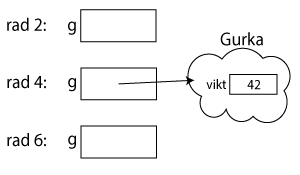
\includegraphics[scale=0.6]{../img/w06-solutions/1b}

\Task % uppgift 2

\Subtask Vi skapar två rymdvarelser, \code{alien} och \code{predator}, med två ben, två armar samt två huvuden (där det ena är skalligt och det andra har hår) vardera. Efter det är varken \code{alien} eller \code{predator} skallig eftersom båda har ett huvud med hår. Sen låter man referensen till \code{predator}s huvud med hår referera till aliens huvud utan hår. Nu är predator helt skallig.

\Subtask  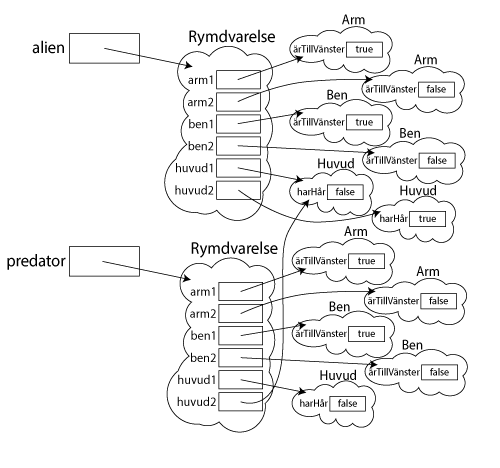
\includegraphics[scale=0.7]{../img/w06-solutions/2b}

\Subtask Eftersom det inte längre finns någon referens som pekar på det objektet kommer Garbage Collector ta hand om det och kommer förr eller senare skrivas över av något annat som behöver sparas. Nej, det går inte att komma åt.

% uppgift 3
\Task Rad 2:
\begin{REPL}
	error: value vikt is not a member of Gurka1
\end{REPL}
Detta eftersom om man varken väljer att skriva \code{val} eller \code{var} skapar inte scala någon getter eller setter (metoder för att läsa/ändra en variabel) och därför ser det ut som att vikt inte finns för kompilatorn.

Rad 4: Denna rad skapar inte en error eftersom om man skriver \code{val} innan variabeln skapas en getter automatiskt och man kan därför komma åt \code{vikt}.

Rad 6:
\begin{REPL}
	error: value vikt in class Gurka3 cannot be accessed in Gurka3
\end{REPL}
I detta fallet skapas en \code{getter} men eftersom accessnivån sätts till \code{private} vet kompilatorn att man inte får komma åt variabeln utifrån.

Rad 11:
\begin{REPL}
	java.lang.NullPointerException
\end{REPL}
Detta eftersom \code{kompis} är \code{ingenGurka} som inte pekar på något objekt och när man då försöker komma åt ett attribut från den kommer det inte funka.

Rad 12: Kommer inte generera en error eftersom när man kallar \code{kompisVikt} (som är \code{public}) försöker den komma åt \code{Gurka4(84, null).vikt}. \code{vikt} är \code{private val} vilket innebär att det har en getter och eftersom huvudobjektet också är av typen \code{Gurka4} är accessnivån tillräckligt hög.

Rad 13:
\begin{REPL}
	error: value vikt is not a member of Gurka5
\end{REPL}
När man sätter ett attribut till \code{private[this]} tillåts inte ens objekt av samma typ att komma åt variabeln och därför får man en error som säger att den inte finns.

Rad 17:
\begin{REPL}
	error: constructor Gurka6 in class Gurka6 cannot be accessed in object
\end{REPL}
Eftersom man satt klassparametrarna till \code{private} kan man inte komma åt konstruktorn och därför får man en error.

Rad 26:
\begin{REPL}
	error: constructor Gurka7 in class Gurka7 cannot be accessed in object
\end{REPL}
Samma anledning som på rad 17.

Rad 27:
\begin{REPL}
	java.lang.IllegalArgumentException: requirement failed: negativ vikt: -42
\end{REPL}
Kompanjonsobjektet har en requirement på att \code{vikt >= 0} vilket innebär att om det inte stämmer kommer man få en error av typen \code{IllegalArgumentException}.

Rad 30: Anledningen till att man kan sätta vikten till något negativt är att checken om det är negativt endast görs när man skapar \code{Gurka7} vilket innebär att i efterhand kan man ändra den till vilket värde som helst (av typen \code{Int}).

\Task % uppgift 4

\Subtask Rad 16:
\begin{REPL}
	java.lang.IllegalArgumentException: requirement failed: negativ vikt: -42
\end{REPL}
Kompanjonsobjektet har en requirement på att \code{vikt >= 0} vilket innebär att om det inte stämmer kommer man få en error.

Rad 20:
\begin{REPL}
	java.lang.IllegalArgumentException: requirement failed: negativ vikt: -1
\end{REPL}
Eftersom settern har implementerat ett krav på att vikten måste vara större eller lika med 0 får man en error när man försöker sätta den till -1.

Rad 22:
\begin{REPL}
	java.lang.IllegalArgumentException: requirement failed: negativ vikt: -958
\end{REPL}
Eftersom 42-1000 är mindre än noll får man en error.

\Subtask Man kan sätta egna mer specifika krav på vad som får göras med värdena så man har större koll på att inget oväntat händer.

% uppgift 5
\Task \begin{CodeSmall}
	class Square(val x: Int, val y: Int, val side: Int) {
		val area: Int = side*side

		def move(dx: Int, dy: Int): Square = new Square(x + dx, y + dy, side)

		def isEqualSizeAs(that: Square): Boolean = this.side == that.side

		def scale(factor: Double): Square = new Square(x, y, (side*factor).toInt)

		override def toString: String = s"Square(x: $x, y: $y, side: $side)"
	}

	object Square {
		val unit: Square = new Square(0, 0, 1)

		def apply(x: Int, y: Int, side: Int): Square = new Square(x, y, side)

		def apply(): Square = new Square(0, 0, 1)
	}
\end{CodeSmall}

Eftersom \code{s1}, \code{s2}, \code{s3} och \code{Square.unit} alla har en sida med längden 1 så kommer rad 3-5 returnera \code{true}. Rad 6 kommer returnera \code{false} eftersom \code{s2.scale(math.Pi)} sida är $\pi$ och \code{s2} fortfarande har sidan 1. Rad 7 kommer däremot returnera \code{true} då båda har sidan $\pi$.

\Task % uppgift 6

\Subtask Variablerna \code{a} och \code{b} är båda objekt av en vanlig klass vilket kommer innebära att de jämförs med referenslikhet och eftersom de inte är samma objekt retunerar \code{==} \code{false}. \code{c} och \code{d} är däremot objekt av en case klass så de jämförs med strukturlikhet och eftersom de har samma vikt returnerar \code{==} \code{true}.

\Subtask Både \code{a eq b} och \code{c eq d} ska returnera \code{false} eftersom de alla är olika objekt och det är referenslikhetsom gäller.

\Task % uppgift 7

\Subtask se e) för komplett lösning

\Subtask se e) för komplett lösning

\Subtask se e) för komplett lösning

\Subtask se e) för komplett lösning

\Subtask \begin{CodeSmall}
case class Point(x: Int, y: Int) {

	def distanceTo(that: Point): Double = math.hypot(that.x - x, that.y -y)

	def distanceTo(x: Int, y: Int): Double = distanceTo(Point(x, y))

	def move(dxdy: (Int, Int)): Point = Point(dxdy._1 + x, dxdy._2 + y)
}

object Point {
	//val origin: Point = new Point(0, 0)
	def origin: Point = Point(0, 0)
}
\end{CodeSmall}

\Subtask \code{==} och \code{!=} kollar strukturlikhet så om två objekt innehåller samma värden kommer \code{==} returnera \code{true} och \code{!=} \code{false} och vise versa. \code{eq} och \code{ne} kollar referenslikhet så om två variabler pekar på samma objekt kommer \code{eq} returnera \code{true} och \code{ne} \code{false} och vise versa.

\Subtask \code{false}. Detta eftersom om origin implementeras som en metod som returnerar en ny \code{Point} varje gång den kallas kommer \code{Point.origin} inte peka på samma objekt varje gång metoden kallas (\code{eq} är referenslikhet).

\Subtask Sturkturlikhet bryr sig endast om innehållet i objekten och jämför det. Det kvittar alltså om det är samma objekt eller två olika så länge de innehåller samma värden. Referenslikhet kollar endast på om det är samma objekt variablerna pekar på och struntar fullständigt i om de innehåller samma värden.

% uppgift 8
\Task \begin{CodeSmall}
class Square(val p: Point, val side: Int) {
	val area: Int = side*side

	def move(dx: Int, dy: Int): Square = new Square(p.move(dx, dy), side)

	def isEqualSizeAs(that: Square): Boolean = this.side == that.side

	def scale(factor: Double): Square = new Square(p, (side*factor).toInt)

	override def toString: String = s"Square(p: $p, side: $side)"
}

object Square {
	val unit: Square = new Square(new Point(0, 0), 1)

	def apply(x: Int, y: Int, side: Int): Square =
		new Square(new Point(x, y), side)

	def apply(): Square = new Square(new Point(0, 0), 1)
}
\end{CodeSmall}

% uppgift 9
\Task  \begin{CodeSmall}
case class Point(p:(Int,Int)) {
	val x: Int = p._1

	val y: Int = p._2

	def distanceTo(that: Point): Double = math.hypot(that.x - x, that.y -y)

	def distanceTo(that: (Int, Int)): Double = distanceTo(Point(that))
	def move(dx: Int, dy: Int): Point = Point(x + dx, y + dy)
}

object Point {
	val origin: Point = new Point(0, 0)
}
\end{CodeSmall}

% uppgift 10
\Task Inget! Eftersom både \code{Point(1,2)} och \code{Point((1,2))} är okej sätt att komma åt den nya klassen så kommer det se likadant utifrån och därför behöver man inte ändra något i \code{Square}.

\Task % uppgift 11

\Subtask \begin{CodeSmall}
class Frog private (initX: Int = 0, initY: Int = 0) {
	private var _x: Int = initX
	private var _y: Int = initY
	private var _distanceJumped: Double = 0

	def jump(dx: Int, dy: Int): Unit = {
		_x += dx
		_y += dy
		_distanceJumped += Math.hypot(dx, dy)
	}

	def x: Int = _x
	def y: Int = _y

	def randomJump: Unit = {
		val r = scala.util.Random
		val xtmp = r.nextInt(10)+1
		val ytmp = r.nextInt(10)+1
		_x += xtmp
		_y += ytmp
		_distanceJumped += Math.hypot(xtmp, ytmp)
	}

	def distanceToStart: Double = Math.hypot(_x,_y)
	def distanceJumped: Double = _distanceJumped
	def distanceTo(that: Frog): Double = Math.hypot(_x - that.x, _y - that.y)
}

object Frog {
	def spawn(): Frog = new Frog()
}
\end{CodeSmall}

\Subtask \begin{CodeSmall}
val f1 = Frog.spawn()
//test requirement 1 and 4
assert(f1.x == 0 && f1.y == 0, "Either x or y isn't 0")

f1.jump(4,3)
//test requirement 1 and 5
assert(f1.x == 4 && f1.y == 3, "Either x isn't 4 or y isn't 3")

f1.jump(4,3)
//test requirement 2
var text = "distanceJumped is " + f1.distanceJumped + ". Should be 10"
assert(f1.distanceJumped == 10, text)

f1.jump(-4,-3)
//test requirement 3
text = "distanceToStart is " + f1.distanceJumped + ". Should be 5"
assert(f1.distanceToStart == 5, text)

var f2 = Frog.spawn()
for (x <- 1 to 1000) {
	f2.randomJump
	//test requirement 5
	text = "Either x or y isn't in [1,10]. x:" + f2.x + ", y: " + f2.y
	assert(f2.x > 0 && f2.x <= 10 && f2.y > 0 && f2.y <= 10, text)
	f2 = Frog.spawn()
}

val f3 = Frog.spawn()
f3.jump(1,1)
val f4 = Frog.spawn()
f4.jump(4,5)
// Test distanceT()
text = "distanceTo is " + f3.distanceTo(f4) + ". Should be 5"
assert(f3.distanceTo(f4) == 5, text)
\end{CodeSmall}

\Subtask Getter

\Subtask Om metoden har parametrar och retur-typen \code{Unit}. Det betyder troligen att parametrarna ändrar något istället för att skapa något nytt.

\Subtask \begin{CodeSmall}
class Frog private (initX: Int = 0, initY: Int = 0) {
	private var _x: Int = initX
	private var _y: Int = initY
	private var _distanceJumped: Double = 0

	def jump(dx: Int, dy: Int): Unit = {
		_x += dx
		_y += dy
		_distanceJumped += Math.hypot(dx, dy)
	}

	def x: Int = _x
	def y: Int = _y

	def x_= (newX: Int): Unit = {
		_distanceJumped += Math.abs(_x - newX)
		_x = newX
	}
	def y_= (newY: Int): Unit = {
		_distanceJumped += Math.abs(_y - newY)
		_y = newY
	}

	def randomJump: Unit = {
		val r = scala.util.Random
		val xtmp = r.nextInt(10)+1
		val ytmp = r.nextInt(10)+1
		_x += xtmp
		_y += ytmp
		_distanceJumped += Math.hypot(xtmp, ytmp)
	}

	def distanceToStart: Double = Math.hypot(_x,_y)
	def distanceJumped: Double = _distanceJumped
	def distanceTo(that: Frog): Double = Math.hypot(_x - that.x, _y - that.y)
}

object Frog {
	def spawn(): Frog = new Frog()
}
\end{CodeSmall}

\Subtask \begin{CodeSmall}
var noCollision = true
var counter = 0
val numberOfFrogs = 100
val distanceBetweenFrogs = 8
val frogArray = Array.fill(numberOfFrogs){Frog.spawn()}
(0 until numberOfFrogs).foreach(i => frogArray(i).x(i*distanceBetweenFrogs))
while (noCollision) {
	frogArray.foreach(frog => frog.randomJump)
	for (frog <- frogArray) {
		for (frog2 <- frogArray) {
			if (frog != frog2 && frog.distanceTo(frog2) < 0.5) {
				noCollision = false
			}
		}
	}
	counter += 1
}
print(counter)
\end{CodeSmall}


\clearpage

\ExtraTasks %%%%%%%%%%%%

\Task

\vspace{1em} %tweak pagination

\begin{CodeSmall}
/** A mutable and expensive Square. */
class Square private (val initX: Int, val initY: Int, val initSide: Int) {

  private var nMoves = 0;
  private var sumCost = 0.0;
  private var _x = initX;
  private var _y = initY;
  private var _side = initSide;

  private def addCost: Unit = {
   sumCost += math.hypot(x - initX, y - initY) * side
  }

  /** The current position on the x axis */
  def x: Int = _x

  /** The current position on the y axis */
  def y: Int = _y

  /** The size of the side */
  def side = _side

  /** Scales the size of this square and rounds it to nearest integer */
  def scale(factor: Double): Unit = { _side = (_side * factor).round.toInt }

  /** Moves this square to position (x + xd, y + dy) */
  def move(dx: Int, dy: Int): Unit = {
    _x += dx; _y += dy;
    nMoves += 1
    addCost
  }

  /** Moves this square to position (x, y) */
  def moveTo(x: Int, y: Int): Unit = {
    _x = x; _y = y;
    nMoves += 1
    addCost
  }

  /** The accumulated cost of this Square */
  def cost: Double = sumCost

  /** Reset the cost of this Square */
  def pay: Unit = {sumCost = 0}

  /** A string representation of this Square */
  override def toString: String =
    s"Square[($x, $y), side: $side, #moves: $nMoves times, cost: $sumCost]"
}

object Square {
  private var created = Vector[Square]()

  /** Constructs a new Square object at (x, y) with size side */
  def apply(x: Int, y: Int, side: Int): Square = {
    require(side >= 0, s"side must be positive: $side")
    val sq = (new Square(x, y, side))
    created :+= sq
    sq
  }

  /** Constructs a new Square object at (0, 0) with side 1 */
  def apply(): Square = apply(0, 0, 1)

  /** The total number of moves that have been made for all squares. */
  def totalNumberOfMoves: Int = created.map(_.nMoves).sum

  /** The total cost of all squares. */
  def totalCost: Double = created.map(_.cost).sum
}
\end{CodeSmall}

\AdvancedTasks %%%%%%%%%

\TODO

%!TEX encoding = UTF-8 Unicode

%!TEX root = ../solutions.tex

\ExerciseSolution{\ExeWeekSIX}


\BasicTasks %%%%%%%%%%%

\Task % Uppgift 1

\Subtask 42;\\
 1\\
 2\\
 7\\
 42;\\
 WrappedArray(hej, på, dej)

\Subtask WrappedArray

\Subtask def printAll(xs: Int*) = {println(xs.size); xs.foreach(println)}

\Subtask Storleken “0” skrivs ut och inget annat.



\Task % Uppgift 2

\Subtask \begin{REPL}
scala.collection.immutable.Vector[IntCell] =
    Vector([Int](7), [Int](42), [Int](9))
\end{REPL}
Referensena till c2 och xs ändras aldrig.
xs kommer fortfarande ha tre vektorer som refererar till c1, c2, c3, däremot refererar dessa i sin tur till var sin int som är Mutable.
I detta fallet ändras c2.x:s referens från 8 till 42.

\Subtask 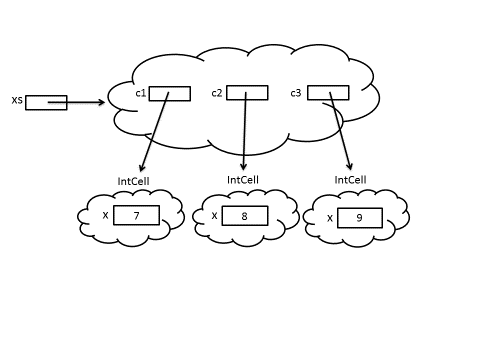
\includegraphics{../img/w05-solutions/memory-pic-1}

\Subtask Istället för att skriva \code{IntCell(var x: Int)} så kan man skriva \code{IntCell(val x: Int)} där varje cells intvärde kommer vara oförändlig.
Alltså då attributen till objekten är “Val” så kommer även de att vara oförändliga.


\Task % Uppgift 3

\Subtask \begin{Code}
def copyAppend(xs: Array[Int], x: Int): Array[Int] = {
  val n = xs.size
  val ys = new Array[Int](n+1)
  var i = 0
  while(i < n) {
    ys(i) = xs(i)
    i += 1
  }
  ys(n) = x
  ys
}
\end{Code}

\Subtask \begin{REPL}
xs: scala.collection.mutable.ArrayBuffer[Int] = ArrayBuffer()
ArrayBuffer(1, 1, 2)
ArrayBuffer(1, 1, 2, 3)
ArrayBuffer(1, 1, 2, 3, 5)
ArrayBuffer(1, 1, 2, 3, 5, 8)
ArrayBuffer(1, 1, 2, 3, 5, 8, 13)
ArrayBuffer(1, 1, 2, 3, 5, 8, 13, 21)
ArrayBuffer(1, 1, 2, 3, 5, 8, 13, 21, 34)
ArrayBuffer(1, 1, 2, 3, 5, 8, 13, 21, 34, 55)
ArrayBuffer(1, 1, 2, 3, 5, 8, 13, 21, 34, 55, 89)
ArrayBuffer(1, 1, 2, 3, 5, 8, 13, 21, 34, 55, 89, 144)
Int = 144
Int = 12
\end{REPL}

\Subtask \code{xs.size = 46}\\
\code{xs(45) = 1836311903}\\
(Ha en arrayBuffer av typen Long istället och byt 100 mot Int.MaxValue och ta det nästsista elementet i sekvensens (det sista kommer vara över))

\Task % Uppgift 4

\Subtask Nej det gör det inte.
Då ys tilldelas xs.toArray kopieras datan från xs över i en array (som är mutable) vilket är en annan referens än den till xs.
Detta innebär att xs och ys inte “pekar” på samma objekt längre.

\Subtask Ja därför båda är array och nu kopieras referensen till ys över till zs.
Därför kommer alla ändringar i zs att påverka ys (så länge de pekar på samma referens).

\Subtask Nej det gör det inte. Se a).


\Task % Uppgift 5

\Subtask Den andra parametern anger hur stor den nya vektorn som returneras ska vara.

\Subtask \begin{enumerate}
\item 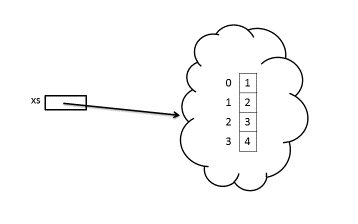
\includegraphics[scale=1.2]{../img/w05-solutions/memory-pic-2}
\item 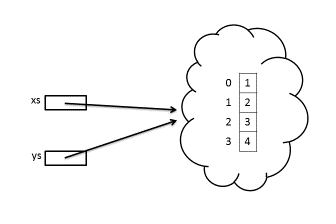
\includegraphics[scale=1.2]{../img/w05-solutions/memory-pic-3}
\item 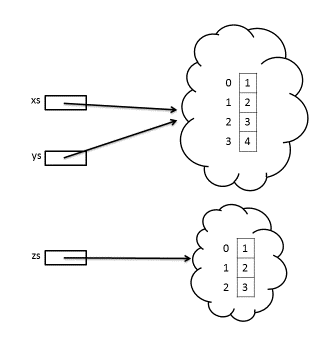
\includegraphics[scale=1.2]{../img/w05-solutions/memory-pic-4}
\item 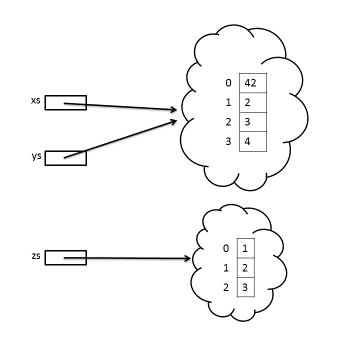
\includegraphics[scale=1.2]{../img/w05-solutions/memory-pic-5}
\item 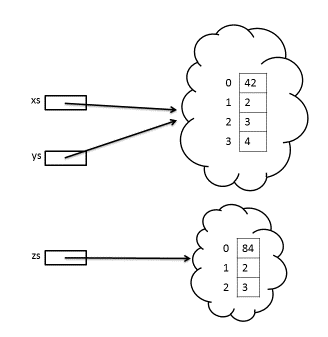
\includegraphics[scale=1.2]{../img/w05-solutions/memory-pic-6}
\end{enumerate}
xs = Array(42, 2, 3, 4)\\
ys = Array(42, 2, 3 ,4)\\
zs = Array(84, 2, 3)\\
\code{xs} och \code{yx} refererar till samma objekt och då deras första IntCell:s värde ändras till 42, så kommer förändringen att ske för båda.
\code{zs} har en referens till ett annat objekt med ett mindre element. Att \code{zs}:s första element ändras, påverkar inte \code{xs} och \code{ys}.


\Task % Uppgift 6

\Subtask \begin{Code}
def seqReverseCopy(xs: Array[Int]): Array[Int] = {
  val n = xs.size
  val ys = Array.fill[Int](n)(0)
  var i = 0
  while(i < n) {
    ys(n-i-1) = xs(i)
    i += 1
  }
  ys
}
\end{Code}

\Subtask \begin{Code}
def seqReverseCopy(xs: Array[Int]): Array[Int] = {
  val n = xs.size
  val ys = Array.fill[Int](n)(0)
  for(i <- n-1 to 0 by -1) ys(n-i-1) = xs(i)
  ys
}
\end{Code}

\Subtask Se b).


\Task % Uppgift 7

\Subtask \begin{Code}
def reverseString(s: String): String = {
  val sb = new StringBuilder(s)
  val n = sb.length
  for (i <- 0 until n / 2) {
    val temp = sb(i)
    sb(i) = sb(n - i - 1)
    sb(n - i - 1) = temp
  }
  sb.toString
}
\end{Code}

\Subtask \begin{Code}
def isPalindrome(s: String): Boolean = {s == reverseString(s)}
\end{Code}

\Subtask \begin{Code}
def isPalindrome(s: String): Boolean = {
  val n = s.length
  var foundDiff = false
  var i = 0
  while (i < n/2 && !foundDiff)  {
    foundDiff = s(i) != s(n - i - 1)
    i += 1
  }
  !foundDiff
}
\end{Code}


\Task % Uppgift 8

\Subtask \code{xs.filter(_ == 6).size}

\Subtask \code{xs.filter(_ % 2 == 0).size}

\Subtask \begin{REPL}
scala.collection.immutable.Map[Int,scala.collection.immutable.Vector[Int]] =
	Map(1 -> Vector(5, 3, 1, 1, 3, 5, 1, 1, 3), 0 -> Vector(6, 6, 2, 6))
scala.collection.immutable.Map[Int,scala.collection.immutable.Vector[Int]] =
	Map(1 -> Vector(5, 3, 1, 1, 3, 5, 1, 1, 3), 0 -> Vector(6, 6, 2, 6))
scala.collection.immutable.Map[Int,scala.collection.immutable.Vector[Int]] =
	Map(2 -> Vector(5, 5, 2), 1 -> Vector(1, 1, 1, 1), 0 -> Vector(3, 6, 3, 6, 3, 6))
(2,Vector(5, 5, 2))
(1,Vector(1, 1, 1, 1))
(0,Vector(3, 6, 3, 6, 3, 6))
freqEvenOdd: scala.collection.immutable.Map[Int,Int] = Map(1 -> 9, 0 -> 4)
nEven: Int = 4
nOdd: Int = 9
\end{REPL}

\Subtask \code{xs.groupBy(i => i)} skapar en map där nycklarna är alla unika element och värdena är av samma värde som respektive nyckel.

\Subtask \code{val freq: Map[Int, Int] = xs.groupBy(i => i).map(p => (p._1, p._2.size))}

\Subtask \begin{Code}
def tärningsRegistrering(xs: Array[Int]): Array[Int] = {
  val f = Array.fill(7)(0)
  f(0) = xs.size
  var i = 0
  while (i < f(0)) {
    f(xs(i)) += 1
    i += 1
  }
  f
}
\end{Code}


\Task % Uppgift 9

\Subtask

\begin{algorithm}[H]
 \SetKwInOut{Input}{Indata}\SetKwInOut{Output}{Resultat}

 \Input{En sekvens $xs$ av typen \texttt{Array[Int]} och $pos$}
 \Output{En ny sekvens av typen \texttt{Array[Int]} som är en kopia av $xs$ fast med elementet på plats $pos$ borttaget}
 $n \leftarrow$ antalet element $xs$\\
 $ys \leftarrow$ en ny \texttt{Array[Int]} med plats för $n-1$ element \\
 \For{$i \leftarrow 0$ \KwTo $pos - 1$}{
  $ys(i) \leftarrow xs(i)$
 }
 $ys(pos) \leftarrow x$ \\
 \For{$i \leftarrow pos+1$ \KwTo $n - 1$}{
  $ys(i - 1) \leftarrow xs(i)$
 }
 \Return $ys$
\end{algorithm}

\Subtask \begin{Code}
def removeCopy(xs: Array[Int], pos: Int): Array[Int] = {
  val n = xs.size
  val ys = Array.fill(n - 1)(0)
  for (i <- 0 until pos) ys(i) = xs(i)
  for (i <- pos+1 until n) ys(i - 1) = xs(i)
  ys
}
\end{Code}


\Task % Uppgift 10

\Subtask

\begin{algorithm}[H]
 \SetKwInOut{Input}{Indata}\SetKwInOut{Output}{Resultat}

 \Input{En sekvens $xs$ av typen \texttt{Array[Int]} och $pos$}
 \Output{En uppdaterad sekvens av $xs$ där elementet på plats $pos$ tagits bort och efterföljande element flyttas ett steg mot lägre index med ett sista elementet som är $0$}
 $n \leftarrow$ antalet element $xs$\\
 \For{$i \leftarrow pos+1$ \KwTo $n - 1$}{
  $xs(i - 1) \leftarrow xs(i)$
 }
 $xs(n - 1) \leftarrow 0$ \\
\end{algorithm}

\Subtask \begin{Code}
def remove(xs: Array[Int], pos: Int): Unit = {
  val n = xs.size
  for (i <- pos+1 until n) xs(i - 1) = xs(i)
  xs(n-1) = 0
}
\end{Code}


\Task % Uppgift 11

\Subtask Antingen kan du skapa en ny instans av \code{java.util.Random} genom att skriva: \code{val r1 = new java.util.Random}.
Men om \code{java.util.Random} importeras kan “java.util” skippas och istället skrivs: \code{val r2 = new Random}.
Som valfritt argument kan ett slumptalsfrö av typen Long skickas med när en ny instans skapas, e.g. \code{val r3 = new Random(42L)}.
\code{nextInt(x)} skapar ett slumptal från och med 0, upp till x (exklusive x).

\Subtask \begin{REPL}
import java.util.Random // Importerar Random

frö: Long = 42 // Ett slumptalsfrö av värdet 42L skapas.

  // Skapar ett Random objekt med slumptalsfrö "frö".
rnd: java.util.Random = java.util.Random@2f410acf

res0: Int = 7 // Slumpade fram ett tal från 0 till och med 9.

9 8 8 8 9 7 2 1 4 0 0 3 8 8 4 5 9 1 3 3 5 1 1
3 3 3 6 3 4 7 5 7 8 7 6 9 7 0 3 0 6 6 1 0 8 1
1 1 0 5 3 5 1 5 3 5 9 9 5 1 8 9 0 6 4 7 5 7 9
6 4 0 8 1 0 9 6 6 3 2 7 9 2 7 0 6 9 8 5 0 0 8
9 2 7 7 3 5 1 3 // Slumpar och skriver ut 100 tal från 0 till och med 9.

  // Skapar ett Random objekt med slumptalsfrö "frö".
rnd1: java.util.Random = java.util.Random@31e4bb20

  // Skapar ett Random objekt med slumptalsfrö "frö".
rnd2: java.util.Random = java.util.Random@45e37a7e

  // Skapar ett Random objekt med slumptalsfrö med
  // värdet av vad tiden är just nu i nanosekunder.
rnd3: java.util.Random = java.util.Random@57eda880

  // Skapar ett Random objekt med slumptalsfrö
  // med värdet (math.random * Long.MaxValue).toLong.
rnd4: java.util.Random = java.util.Random@79da1ec0

flip: (r: java.util.Random)String // Skapar en funktion som singlar slant.

  // Singlar slant med alla fyra Random
  // objekt 100 gånger samt printar ut resultatet.
xs: scala.collection.immutable.IndexedSeq[(String, String, String, String)] =
Vector((krona,krona,krona,klave), (klave,klave,krona,krona), (krona,krona,klave,klave),
(klave,klave,krona,klave), (klave,klave,krona,krona), (krona,krona,klave,krona),
(klave,klave,klave,klave), (krona,krona,klave,krona), (krona,krona,klave,krona),
(klave,klave,krona,klave), (krona,krona,krona,klave), (klave,klave,krona,klave),
(klave,klave,krona,krona), (klave,klave,klave,krona), (klave,klave,klave,krona),
(krona,krona,klave,klave), (klave,klave,klave,klave), (krona,krona,klave,krona),
(krona,krona,klave,klave), (krona,krona,klave,klave), (krona,krona,klave,krona),
(klave,klave,klave,klave), (klave,klave,krona,krona), (klave,klave,klave,klave),
(krona,krona,krona,krona), (krona,krona,krona,klave)...

  // Kollar om det finns något värde som rnd1
  // har genererat men som inte rnd2 genererat.
res1: Boolean = false

  // Kollar om det finns något värde som rnd1
  // har genererat men som inte rnd3 genererat.
res2: Boolean = true

\end{REPL}

\Subtask Vid felsökning och vid simulering där man vill att samma “slumpmässiga” sekvens uppstår varenda gång.

\Subtask Ja.

\Subtask \url{https://docs.oracle.com/javase/7/docs/api/java/lang/Math.html#random%28%29--} säger att den skapar ett nytt java.util.Random-objekt.

\Subtask Den skapar ett slumpmässigt slumptalsfrö. För mer information, se: \url{https://docs.oracle.com/javase/8/docs/api/java/util/Random.html#Random--}


\Task % Uppgift 12

\begin{Code}
def testRandom(r: Random, n: Int): Unit = {
  val xs = Array.fill(n)(r.nextInt(6) + 1)
  val f = tärningsRegistrering(xs)
  println("Antal kast: " + f(0))
  for (i <- 1 to 6) println(s"Antal $i:or: " + f(i))
}
\end{Code}


\Task % Uppgift 13

\Subtask -

\Subtask \begin{REPL}
Rolling the dice 10000 times with seed 42
Number of 1's: 1654
Number of 2's: 1715
Number of 3's: 1677
Number of 4's: 1629
Number of 5's: 1643
Number of 6's: 1682
\end{REPL}
Simulerar 10000 tärningskast (med slumptalsfrö 42) och skriver ut förekomsten av respektive tärningskast.

\Subtask Array i scala deklararas: \code{val scalaArray = Array.ofDim[Int](6)} medan i java skrivs: \code{int[] javaArray = new int[6];}
\code{for}-sats i scala skrivs: \code{for(i <- 0 to n)} medan i java skrivs: \code{for (int i = 0; i < n; i++)}.
I java måste semicolon skrivas efter varje operation samt att typen måste explicit definieras vid variabeldeklaration.
I scala behövs inga semicolon (förutom för att separera operationer på samma rad) och scala bestäms typen implicit, alltså att kompilatorn “gissar” typen av variabeln som deklareras.

\Subtask Lägg till \code{System.out.println(i);} i for-looparna

\Subtask \begin{Code}[language=Java]
// DiceReg2.java
import java.util.Random;
public class DiceReg2{
	public static int[] diceReg = new int[6];
	private static Random rnd = new Random();

	public static int parseArguments(String[] args){
		int n = 100;
		if(args.length > 0) {
			n = Integer.parseInt(args[0]);
		}
		if(args.length > 1) {
			int seed = Integer.parseInt(args[1]);
			rnd.setSeed(seed);
		}
		return n;
	}

	public static void registerPips(int n) {
		for(int i = 0; i<n; i++) {
			int pips = rnd.nextInt(6);
			diceReg[pips]++;
		}
	}

	public static void main(String[] args) {
		int n = parseArguments(args);
		registerPips(n);
		printReg();
	}
}
\end{Code}

\Subtask \begin{REPL}
  // Skriver ut förekomsten av 1000 tärningskast med slumptalsfrö 42.
Number of 1's: 165
Number of 2's: 163
Number of 3's: 178
Number of 4's: 183
Number of 5's: 156
Number of 6's: 155

  // Skriver ut diceReg-attributet
res1: Array[Int] = Array(165, 163, 178, 183, 156, 155)

  // Skriver ut diceReg-attributet efter 1000 till kast.
res2: Array[Int] = Array(329, 325, 349, 360, 324, 313)

  // Skriver ut diceReg-attributet efter 1000 till kast.
res3: Array[Int] = Array(498, 484, 531, 513, 485, 489)

  // Det blir runtime error då attributet rnd är
  // private och kan inte nås via REPL:n.
<console>:11: error: value rnd is not a member of object DiceReg2
	DiceReg2.rnd
				    ^
\end{REPL}

\Subtask \begin{REPL}
value [diceReg/rnd] is not a member of object DiceReg2
\end{REPL}

\Subtask Om man ska spara under någon data som man inte vill att användaren, eller någon annan, inte ska kunna komma åt.
T.ex. om du gör en bankapp vill du inte att nyckeln som du använder för att autorisera en användare ska vara tillgänglig för då kan hackare använda det för att ta sig in på kontot och stjäla pengar!


\Task % Uppgift 14

\Subtask \code{hasNextInt()} kollar enbart om det finns ett till tal och returnerar \code{true}/\code{false}. \code{nextInt()} “hoppar” till nästa tal och returnerar det.
Se \url{https://docs.oracle.com/javase/7/docs/api/java/util/Scanner.html#hasNextInt%28%29} och \url{https://docs.oracle.com/javase/7/docs/api/java/util/Scanner.html#nextInt%28%29 }.

\Subtask -

\Subtask -

\Subtask \begin{Code}[language=Java,numbers=left]
import java.util.Random;
import java.util.Scanner;

public class DiceScanBuggy {
	public static int[] diceReg = new int[6];
	public static Scanner scan = new Scanner(System.in);

	public static void registerPips() {
		System.out.println("Enter pips separated by blanks: ");
		System.out.println("End with -1 and <Enter>.");
		boolean isPips = true;
		while(isPips && scan.hasNextInt()){
			int pips = scan.nextInt();
			if(pips >= 1 && pips <= 6) {
				diceReg[pips-1]++;
			} else {
				isPips = false;
			}
		}
	}

	public static void printReg(){
		for(int i = 1; i<7; i++) {
		System.out.println("Number of " + i + "'s: " + diceReg[i-1]);
		}
	}

	public static void main(String[] args) {
		registerPips();
		printReg();
	}
}
\end{Code}

\Task % Uppgift 15

\Subtask \code{ArrayBuffer}.

\Subtask \code{ArrayBuffer} eller \code{Array}.

\Subtask \code{Array}.

\Subtask \code{Vector}.



\ExtraTasks %%%%%%%%%%%%

\Task % Uppgift 16

\Subtask \begin{Code}
def insertCopy(xs: Array[Int], x: Int, pos: Int): Array[Int] = {
  val n = xs.size
  val ys = Array.ofDim[Int](n + 1)
  for (i <- 0 until pos) ys(i) = xs(i)
  ys(pos) = x
  for (i <- pos until n) ys(i + 1) = xs(i)
  ys
}
\end{Code}

\Subtask \code{pos} måste vara \code{0}.

\Subtask \begin{REPL}
java.lang.ArrayIndexOutOfBoundsException: -1
\end{REPL}

\Subtask Elementet \code{x} läggs till på slutet av arrayen, alltså kommer den returnerande arrayen vara större än den som skickades in.

\Subtask \begin{REPL}
java.lang.ArrayIndexOutOfBoundsException: 5
\end{REPL}
Man får \code{ArrayIndexOutOfBoundsException} då indexeringen är utanför storleken hos arrayen.

\Task % Uppgift 17

\Subtask

\begin{algorithm}[H]
 \SetKwInOut{Input}{Indata}\SetKwInOut{Output}{Resultat}

 \Input{En sekvens $xs$ av typen \texttt{Array[Int]} och heltalen $x$ och $pos$}
 \Output{En uppdaterad sekvens av $xs$ där elementet $x$ har satts in på platsen $pos$ och efterföljande element flyttas ett steg där sista elementet försvinner}
 $n \leftarrow$ antalet element $xs$\\
 $ys \leftarrow$ en klon av $xs$\\
 $xs(pos) \leftarrow x$\\
 \For{$i \leftarrow pos+1$ \KwTo $n - 1$}{
  $xs(i) \leftarrow ys(i - 1)$
 }
\end{algorithm}

\Subtask \begin{Code}
def insert(xs: Array[Int], x: Int, pos: Int): Unit = {
  val n = xs.size
  val ys = xs.clone
  xs(pos) = x
  for (i <- pos + 1 until n) xs(i) = ys(i - 1)
}
\end{Code}


\Task % Uppgift 18

\begin{Code}
def tärningsRegistrering(xs: Array[Int]): Array[Int] = {
  val f = Array.fill(7)(0)
  f(0) = xs.size
  for(i <- 0 until f(0)) f(xs(i)) += 1
  f
}
\end{Code}


\Task % Uppgift 19



\AdvancedTasks %%%%%%%%%


\Task % Uppgift 20

\Subtask

\Subtask


\Task % Uppgift 21

\Subtask

\Subtask

\Subtask


\Task % Uppgift 22


\Task % Uppgift 23

\Subtask

\Subtask

\Subtask

%!TEX encoding = UTF-8 Unicode

%!TEX root = ../solutions.tex

\ExerciseSolution{\ExeWeekFOUR}

\Task %Uppgift 1

\Subtask  
\begin{REPLnonum}
scala> val pt = (15.9, 28.9)

scala> math.hypot(pt._1, pt._2)
res0: Double = 32.98514817307935
\end{REPLnonum}

\Subtask  \code{val (x, y) = pt}

\Subtask  \code{(String, String, Double, Boolean)}

\Subtask  \code{Vector[(Double, Double)]}

\Subtask  \code{huvudstäder :+ ''Danmark'' -> ''Köpenhamn''}

\Subtask  \code{Vector[Double]}

\Subtask  \code{val antalUdda = (1234 to 3456).map(i => div(i, 2)._2).sum}

\Subtask  0-tupel

\Task %Uppgift 2

\Subtask  \code{mittKonto.saldo = (math.random * 1000000).toInt}

\Subtask  Går ej eftersom val är oförändlig, man får alltså ett Error.

\Task %Uppgift 3

\Subtask  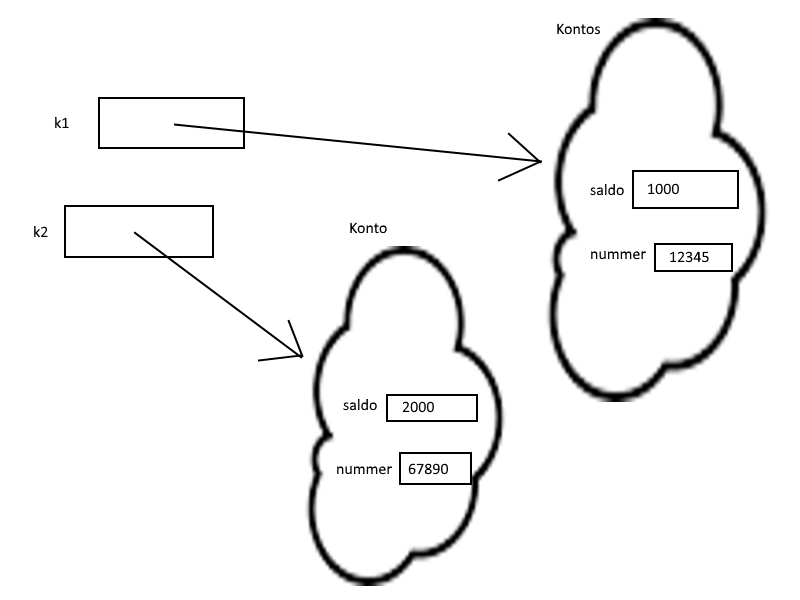
\includegraphics[scale=0.5]{../img/w04-solutions/uppgift-3a}

\Subtask  
Tilldelningen på rad 8 \code{k1.nummer = 12345L} ger felmeddelande eftersom variablen är oförändlig.

\Task %Uppgift 4

\Subtask  \code{String = Konto@cd576}, där \code{Konto@cd576} är ett unikt namn som identifierar instansen.

\Subtask  Ja.

\Subtask  
\begin{REPLnonum}
scala> k.saldo = 42
scala> k2.saldo = 67
\end{REPLnonum}

\Subtask  Eftersom variablen är oförändlig ges ett felmeddelande.

\Subtask  En fördel med klass är att man kan specificera att variablen ska kunna vara förändlig. En till är att man kan inkludera metoder i klassen som man vill kunna använda på värdena.

\Task %Uppgift 5

\Subtask 
Det går bra att ändra på variablen saldo i instansen av Konto1 men inte av Konto2 där man får ett error på raden ''k2.saldo += 1000''

\Subtask -

\Subtask 
''println(k.saldo)'' och ''k.saldo += 1000'' ger båda error, pga privat attribut.

\Subtask 
\begin{Code}
def ut(belopp: Int): (Int, Int) = {
	if(saldo >= belopp) {
		saldo -= belopp
		(belopp, saldo)
	} else {
		val temp = saldo
		saldo = 0
		(temp, 0)
	}
}
\end{Code}

\Subtask 
Lägg till en if-sats i båda funktionerna som omsluter den gamla koden.
\begin{Code}
def ut(belopp: Int): (Int, Int) = {
  if(belopp >= 0) {
    if(saldo >= belopp) {
      saldo -= belopp
      (belopp, saldo)
    } else {
      val temp = saldo
      saldo = 0
      (temp, 0)
    }
  }
}

def in(belopp: Int): Unit = {
  if(belopp >= 0) {
    saldo += belopp 
  }
}
\end{Code}

\Subtask 
Genom att göra attributet privat och gör egna metoder kan man se till att attriuten endast ändras på säkra sätt. Så inte fel uppstår.

\Task %Uppgift 6

\Subtask 
''val i: Int = pt.x'' error: type mismatch;
Eftersom typen Int ej är kompatibel med ett värde av typen Double.

''val p: Double = new Punkt(5.0, 5.0)'' error: type mismatch;
Eftersom typen Double ej är kompatibel med ett värde av typen Punkt.

''val p = new Punkt(5.0, 5.0): Double'' error: type mismatch;
Eftersom typen Double ej är kompatibel med ett värde av typen Punkt.

\Subtask 
Rad 3 till 7 i respektive ordning: true, false, false, true och false.

\Task %Uppgift 7
\\En variabel med namn pt skapas med typen Punkt.\
\\true
\\true
\\String = 1.0
\\skriver ut: 1.0
\\error: not found: value a
\\String = 2.0
\\error: not found: value a

\Task %Uppgift 8

\Subtask 
''println(pt)'' kallar på pt.toString, och eftersom metoden är överskriven kallas den nya version.

\Subtask  \code{override def toString: String = ''Punkt('' + x + '', '' + y + '').''}

\Subtask 
error: overriding method toString in class Object of type ()String;

\Task %Uppgift 9

\Subtask 
\begin{REPL}
scala> val pt = Pt(1.0, 2.0)
pt: Pt = Pt(x=1.0,y=2.0)

scala> Pt(4.0, 2.0)
res0: Pt = Pt(x=4.0,y=2.0)

scala> Pt(6.0, 3.0)
res1: Pt = Pt(x=6.0,y=3.0)

scala> Pt(666.0, 1337.0)
res2: Pt = Pt(x=666.0,y=1337.0)
\end{REPL}

\Subtask \code{def apply(): Pt = new Pt(0, 0)}

\Subtask \code{class Rational(val nom: Int, val denom: Int)}

\Subtask 
\begin{REPLnonum}
object Rational { 
def apply(nom: Int, denom: Int): Rational = new Rational(nom, denom)
}
\end{REPLnonum}

\Subtask 
\begin{REPL}
scala> Rational(2, 5)
scala> Rational(2, 7)
scala> Rational(7, 4)
scala> Rational(666, 1337)
\end{REPL}

\Task %Uppgift 10
\Subtask \code{case class Rational(nom: Int, denom: Int)}

\Task %Uppgift 11

\Subtask 
\begin{REPLnonum}
scala> Point(3, 4).distToOrigin
res0: Double = 5.0
\end{REPLnonum}

\Subtask 
p3.x = 8
p3.y = 10

\Task %Uppgift 12

\Subtask 
\\Operatornotation:	4, 6, 10, 12
\\Punktnotation:		3, 5, 8, 9, 11, 13
\\Felmeddelande:		9

\Subtask
\begin{Code}
case class Point(x: Double, y: Double) {
  def distToOrigin: Double = math.hypot(x, y)
  def add(p: Point): Point = Point(x + p.x, y + p.y)
  def +(p: Point): Point = add(p)
  def sub(p: Point): Point = Point(x - p.x, y - p.y)
  def -(p: Point): Point = sub(p)
}
\end{Code}
\begin{REPL}
scala> val p1: Point = Point(1, 9)
scala> val p2: Point = Point(9, 6)
scala> p1.sub(p2)
scala> p1.-(p2)
scala> p2 sub p1
scala> p2 - p2
scala> p1.add(p2.sub(p1))
scala> p1 + (p2 - p1)
\end{REPL}

\Subtask
\begin{Code}
case class Point(x: Double, y: Double) {
  def distToOrigin: Double = math.hypot(x, y)
  def add(p: Point): Point = Point(x + p.x, y + p.y)
  def +(p: Point): Point = add(p)
  def sub(p: Point): Point = Point(x - p.x, y - p.y)
  def -(p: Point): Point = sub(p)
  def scale(a: Double, b: Double) = Point(x * a, y * b)
}
\end{Code}
\begin{REPL}
scala> val p: Point(13,  37)
scala> p.scale(4, 2)
scala> p scale (3, 7)
\end{REPL}

\Task %Uppgift 13

\Subtask  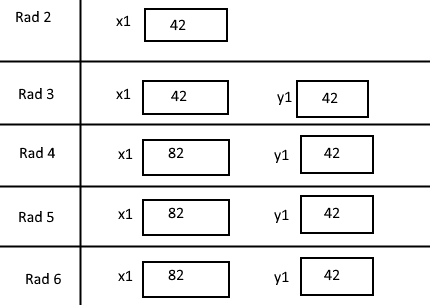
\includegraphics[scale=0.5]{../img/w04-solutions/uppgift-13a}

\Subtask  
\begin{enumerate}
\item 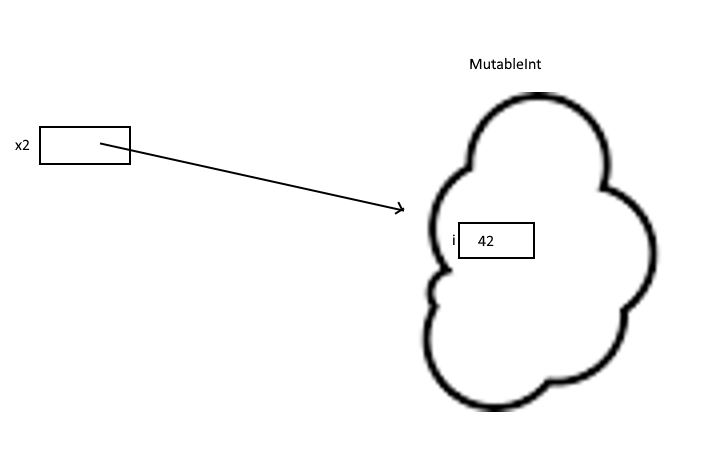
\includegraphics[scale=0.5]{../img/w04-solutions/uppgift-13b-1}
\item 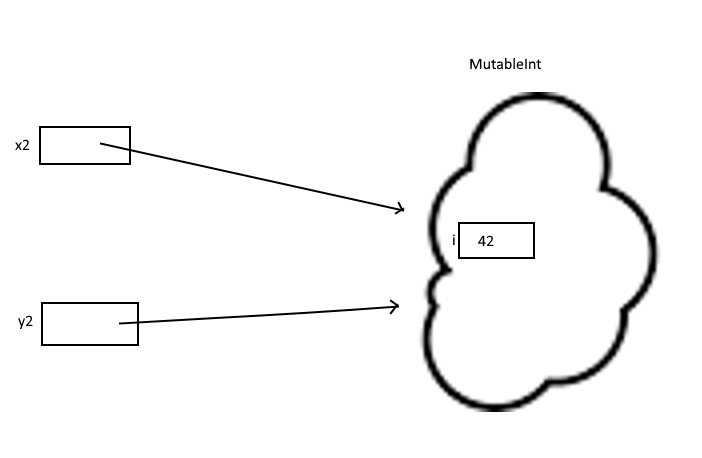
\includegraphics[scale=0.5]{../img/w04-solutions/uppgift-13b-2}
\item 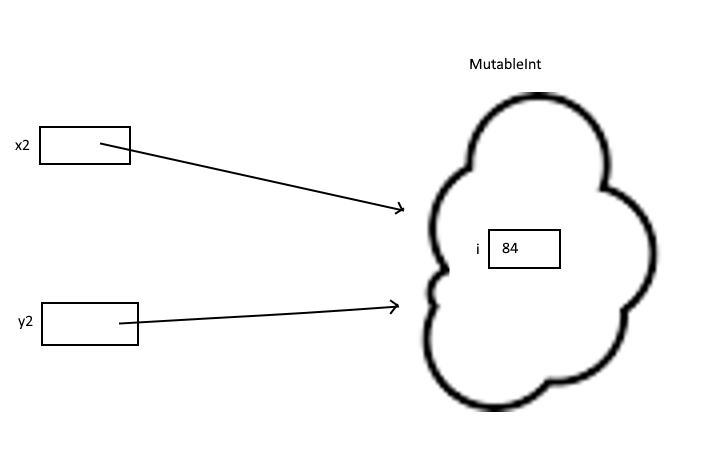
\includegraphics[scale=0.5]{../img/w04-solutions/uppgift-13b-3}
\end{enumerate}

\Subtask  
\begin{enumerate}
\item 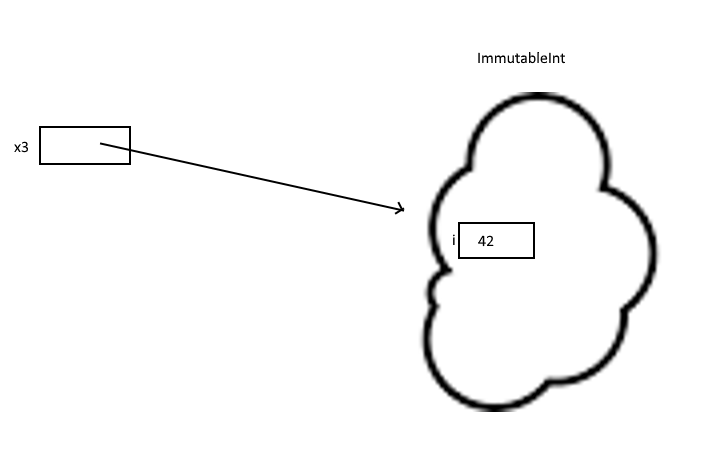
\includegraphics[scale=0.5]{../img/w04-solutions/uppgift-13c-1}
\item 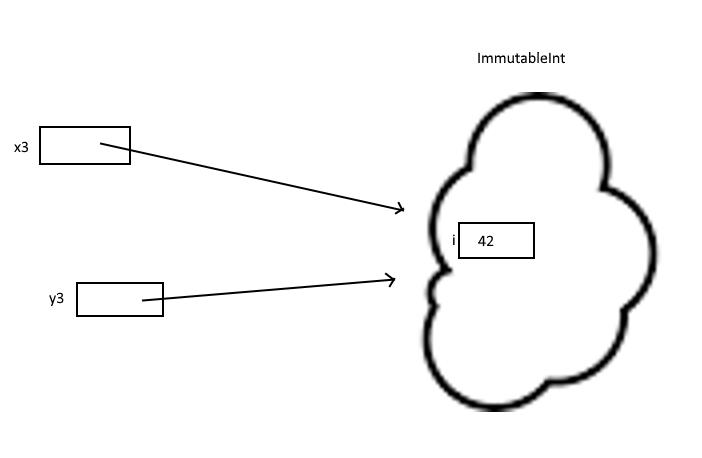
\includegraphics[scale=0.5]{../img/w04-solutions/uppgift-13c-2}
\item 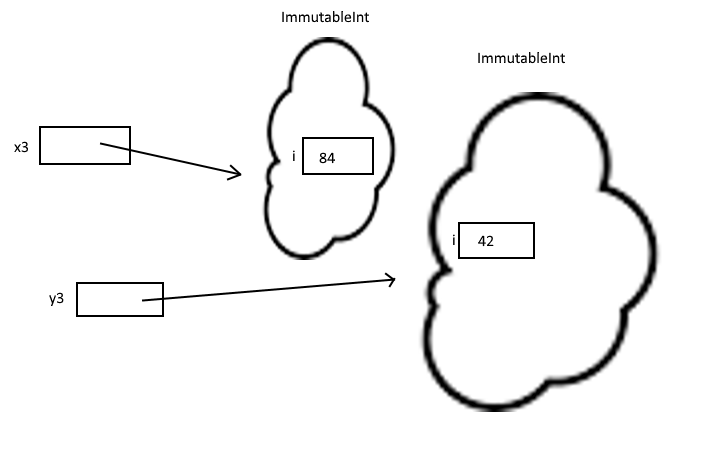
\includegraphics[scale=0.5]{../img/w04-solutions/uppgift-13c-3}
\end{enumerate}

\Subtask  En stor fördel är att vi till exempel kan skicka med en immutable som argument till en metod och vara säkra på att metoden inte ändrar på värdet.

\Task %Uppgift 14

\Subtask  Ungefär 150 metoder.

\Subtask  Ungefär lika många.

\Task %Uppgift 15

\Subtask 
\\1. Instansierar en tom vektor med element av typen int och tilldelar värdet till en variabel xs.
\\2. Error eftersom \code{xs :+ ''42''} ger en Vector[Any] när Vector[Int] krävs.
\\3. xs tilldelas ett nytt värde av Vector(43, 64, 46)
\\4. xs skrivs ut.
\\5. Lägger till talet 42 i xs.
\\6. Error: type mismatch
\\7. Skapar en tom Vector i variablen ingenting
\\8. ingenting får värdet Vector(1, 2, 3)

\Subtask 
Tre metoder skapas, första för att få första elementet i en lista, och eftersom den defineras med special typen T går den att använda med alla Vektorer oavsätt typen av variable i vektorn. Den andra får fram sista elementet och sista hämtar båda två.

En till function defineras längre ner ''wrap'', som tar en lista och lägger till ett element längst fram och ett längst bak.

\Task %Uppgift 16

\Subtask  String = ''ka2''

\Subtask  String = ''abra''

\Subtask  false

\Subtask  false

\Subtask  100000

\Subtask  100000

\Subtask  minsta talet i listan

\Subtask  största talet i listan

\Subtask  1

\Subtask  3

\Subtask  Vektor b fast med ''först'' som första element

\Subtask  Vektor a fast med ''sist'' som sista element.

\Subtask  plats 3 i vektorn xs får värdet 42

\Subtask  En ny vektor fylld med ''!'' från och med plats 4 till 10. Men de andra värdena samma som i a.

\Subtask  b sorterad i bokstävsordning

\Subtask  b baklänges

\Subtask  true

\Subtask  true

\Subtask  en vektor med alla unika element i b.

\Task %Uppgift 17

\Subtask 
Metoden ger tillbaka en ny Vector[String] som nu består av alla element i a plus alla element i b. I samma ordning med elementen i a först.

\Subtask 
Samma som i uppgift a fast vektorn som returnas är av typen Vector[Any]. Det är eftersom Any är den närmsta typen som String och Double delar. Elementen från vektor a är fortfarande först och uppföljt av elementen i stor.

\Subtask 
Variablen ys får värdet av en Vector[Int] som innehåller alla talen från xs fast multiplicerade med 5. Alltså ys = 5, 10, 15..., osv.

\Subtask 
Functionen tar alla värden från en Vektor och sätter in i ett Set (mängd). Eftersom en mängd ej har dubletter så försvinner ett ''sala'' och ett ''bim'', Vector[String] som returneras blir därför (''sim'', ''sala'', ''bim'').

\Subtask 
Metoden head ger första elementet i en samling, och last sista. Därför blir kombinationen av a.head och b.last en ny Vector[String] som består av a:s första element, och b:s första element.

\Subtask 
Ger en Vector[String] som innehåller alla element efter det första. Alltså i detta fallet ''ka'' och ''dabra''.

\Subtask 
True, eftersom head ger första elementet och tail ger resten, sedan sätter metoden +: ihop dem till en vektor med samma värden som a.

\Subtask 
Eftersom ++ sätter ihop alla värden från två vektorer måste vi först omvandla från en sträng till vektor. Resultatet blir en ny vektor av samma typ som innan med a:s första element och b:S sista.

\Subtask 
Samma resultat som i h, metoden take börjar från vänster och tar så många element som man skickar med som parameter och gör till en ny lista. Med 1 som parameter motsvarar det att göra Vector(a.head). Metoden takeRight gör samma sak fast från höger.

\Subtask 
Metoden drop är motsvarigheten till take fast excuderar de speciferade elementen istället för att inkludera dem i vektorn.

\Subtask 
Eftersom a endast innehåller 3 element returnerar drop(100) en tom vektor.

\Subtask 
Returnerar en tom vektor med element typen String

\Subtask 
returnerar Vector(true, false) 

\Subtask 
True, metoden contains kollar om en samling innehåller ett specifikt element.

\Subtask 
True. Eftersom en sträng även kan ses som Vector[Char].

\Subtask 
Filtrerar vektorn a till att endast innehålla strängar som innehåller k.

\Subtask 
Exakt samma som i p

\Subtask 
map(\_.toUpperCase) omvandlar alla strängar i a till stora bokstäver
filterNot(\_.contains(''K'')) tar resultatet vi precis fick och tar bort alla strängar som innehåller stora K.

\Subtask 
filtrerar så att endast jämna tal finns kvar.

\Subtask 
Exakt samma som i s



\Task %Uppgift 18

\Subtask 
Vi instansierar en vektor xs med talen 1, 2 och 3.
sedan definerar vi en metod blandat som ger oss en randomiserad version av xs.
sedan definerar vi en till metod som testar om xs är lika med resultatet från blandat. Om det är så returnerar den strängen ''lika'' annars ''olika''.
Sist kör vi en for-loop där vi 100 gånger kör testet, samtidigt räknas hur många gånger ''lika'' returneras.

Vårt resultat är en siffra på hur många gånger xs var samma som en blandad version av sig själv, eftersom det finns 6 permutationer med 3 variabler så borde det vara ungefär 1/6 chans.

\Subtask -

\Subtask 
\\ \code{map(\_.trim)} tar bort alla onödiga mellanrum i början och slutet på varje rad
\\ \code{filterNot(\_.startsWith(''<''))} filtrerar bort alla rader som börjar med strängen ''<''
\\ \code{filterNot(\_.isEmpty)} filtrerar bort alla tomma rader.
\\ \code{foreach(println)} skriver ut alla rader.

\Task %Uppgift 19

\Subtask 
I princip alla metoder delas, en lista har några fler t. ex. ''::'', '':::'', ''mapConserve'' osv.

\Subtask 
Först skapas en lista med 4 sträng värden och instansierar variablen xs med det värdet.
sedan skapar vi en ny lista, som består av ''zero'' + den gamla listan och ger värdet till xs.
Sist instansierar vi en ny variabel ys, som får värdet av xs omvänd plus xs.

\Task %Uppgift 20

\Subtask 
true, Boolean

\Subtask 
En samling av alla värden i s och t, Set[String]

\Subtask 
true, Boolean

\Subtask 
false, Boolean

\Subtask 
false, Boolean

\Subtask 
false, Boolean

\Subtask 
true, Boolean

\Subtask 
Samlingen s utan elementet ''Stockholm'', Set[String]

\Subtask 
Samlingen t utan elementen ''Norge'' och ''Danmark'', Set[String]

\Subtask 
returnerar s, Set[String]

\Subtask 
Samlingen s utan ''Malmö'' och ''Oslo'', Set[String]

\Subtask 
Set(2, 3), Set[Int]

\Subtask 
se deluppgift l

\Subtask 
Set(1, 2, 3 ,4), Set[Int]

\Subtask 
se deluppgift n

\Task %Uppgift 21

\Subtask 
Returnerar strängen ''Malmö'' eftersom det värdet är indexerat på platsen ''Skåne''.

\Subtask 
Returnerar strängen ''Stockholm'' eftersom det värdet är indexerat på platsen ''Sverige''.

\Subtask 
true, eftersom huvudstar innehåller indexet ''Skåne''

\Subtask 
false, eftersom huvudstad ej innehåller indexet ''Malmö''. Notera att det är index och inte värden vi 
kollar om det finns.

\Subtask 
Lägger till indexet ''Danmark'' med värdet ''Köpenhamn'' i samlingen.

\Subtask 
Skriver ut alla 2-tupler.

\Subtask 
Returnerar ''Oslo'', Note: Om indexet ''Norge'' inte hade funnits hade ''???'' returnerats istället.

\Subtask 
Returnerar ''???''

\Subtask 
Returnerar en sorterar vektor med alla index.

\Subtask 
Returnerar en sorterar vektor med alla värden.

\Subtask 
Returnerar en ny mängd men med ''Skåne'' -> ''Malmö'' borttaget. 

\Subtask 
Returnerar huvudstad mängden eftersom det inte finns ett ''Jylland'' index att ta bort.

\Subtask 
Uppdaterar indexet ''Skåne'' till att istället leda till värdet ''Lund''

\Task %Uppgift 22

\Subtask 
\begin{REPLnonum} 
pairs: scala.collection.immutable.Vector[(String, Long)] = 
					Vector((Björn,444), (Maj,441), (Lucy,666))
\end{REPLnonum}

\Subtask 
Map[String, Long]

\Subtask 
\begin{REPLnonum}
scala> telnr(''Maj'')
res0: Long = 441

scala> telnr.get(''Maj'')
res1: Option[Long] = Some(441)

scala> telnr(''Kim'')
java.util.NoSuchElementException: key not found: 'Kim
  at scala.collection.MapLike$class.default(MapLike.scala:228)
  at scala.collection.AbstractMap.default(Map.scala:59)
  at scala.collection.MapLike$class.apply(MapLike.scala:141)
  at scala.collection.AbstractMap.apply(Map.scala:59)
  ... 32 elided

scala> telnr.get(''Kim'')
res2: Option[Long] = None
\end{REPLnonum}

\Subtask 
\begin{REPLnonum} 
scala> telnr.getOrElse(''Maj'', -1L)
res0: Long = 441

scala> telnr.getOrElse(''Kim'', -1L)
res1: Long = -1
\end{REPLnonum} 

\Subtask 
telnr += ''Fröken Ur'' -> 464690510L

\Subtask 
telnr.toVector.map(p => p.\_1 -> (''0'' + p.\_2.toString.substring(2)))

\Subtask 
Använd metoden toMap och apply.



\Task %Uppgift 23

\Subtask  Metoden maxBy hämtar det element som är ''störst'', på rad två gör \code{x => x._1} att första värdet i tuplerna används för att bestämma vilken som är störst. Likt gör \code{x => x._2} på rad tre att istället det andra värdet används.

\Subtask  
\begin{REPLnonum}
scala> xs.maxBy(_._1)
scala> xs.maxBy(_._2)
\end{REPLnonum}

\Subtask  
\begin{REPLnonum}
scala> xs.minBy(_._1)
scala> xs.minBy(_._2)
\end{REPLnonum}


\Task %Uppgift 24

Metoden \code{sliding(i: Int).toVector} skapar en ny vector med alla möjliga permutationer av elementen i en vektor med storleken i.

%!TEX encoding = UTF-8 Unicode

%!TEX root = ../solutions.tex

\ExerciseSolution{\ExeWeekEIGHT}

\BasicTasks %%%%%%%%%%%

%Uppgift 1
\Task

%1.a)
\Subtask  
\includegraphics{../img/w09-solutions/1a} \\
Typ: \code{Vector[Vector[Int]]}\\
Värde: \code{Vector(Vector(1, 2, 3, 4, 5), Vector(3, 4, 5, 6, 7))} \\
Dimensioner: $2 \times 5$\\
Inom matematiken sker indexering enligt konvention med 1 som lägsta index. I scala är lägsta index 0, man använder s.k. 0-indexering. \footnote{Detta är inte fallet i alla programmeringsspråk, vilket du kan läsa mer om på \url{https://en.wikipedia.org/wiki/Array\_data\_type\#Index\_origin}}

%1. b)
\Subtask \\
2: \code{Int}\\
3: \code{Vector[Int]}\\
4: \code{Int}

%1.c)
\Subtask \\
m2: \code{Vector[Vector[Int]]}\\
m3: \code{Vector[Vector[AnyVal]]}\\
m4: \code{Vector[Vector[Any]]}\\
m5: \code{Vector[Vector[Int]]}

%1.d)
\Subtask TODO

%1.e)
\Subtask m5, $42 \times 2$

%Uppgift 2
\Task

%2.a)
\Subtask \begin{Code}
def throwDie: Int = (math.random * 6).toInt + 1
\end{Code}

%2.b)
\Subtask $1000 \times 5$

%2.c)
\Subtask -- %Inget svar

%2.d)
\Subtask \begin{Code}
def roll(n: Int) = Vector.fill(n)(throwDie).sorted
\end{Code}

%2.e)
\Subtask \begin{Code}
def isYatzy(xs: Vector[Int]): Boolean = xs.forall(_ == xs(0))
\end{Code}

%2.f)
\Subtask \begin{Code}
def isYatzy(xs: Vector[Int]): Boolean = {
	var foundDiff = false
	var i = 0
	while (i < xs.size && !foundDiff) {
		foundDiff = xs(i) != xs(0)
		i += 1
	}
	!foundDiff
}
\end{Code}

%2.g)
\Subtask \begin{Code}
def diceMatrix(m: Int, n: Int): Vector[Vector[Int]] =
  Vector.fill(m)(roll(n))
\end{Code}

%2.h)
\Subtask \begin{Code}
def diceMatrixToString(xss: Vector[Vector[Int]]): String =
  xss.map(_.mkString(" ")).mkString("\n")
\end{Code}

%2.i)
\Subtask Funktionen går igenom varje matrisrad, där den i sin tur går igenom
varje element på raden och lägger till i \code{StringBuilder}-objektet. Om det inte är
det sista elementet på raden läggs även ett blanktecken till, annars läggs ett
nyradstecken till. Undantaget är sista raden, där inget nyradstecken läggs till.
Slutligen konverteras \code{StringBuilder}-objektet till en \code{String} som
returneras.\\
Är \code{xss} tom utvärderas \code{0 until xss.size} till en tom \code{Range}
eftersom \code{xss.size} blir \code{0} och \code{until} är exkluderande.
Innehållet i den yttre \code{for}-loopen hoppas över och en tom sträng returneras.
Är alla rader tomma hoppas i stället de inre \code{for}-looparna över, med samma resultat.\\
Med \code{StringBuilder} behöver inte hela innehållet kopieras vid varje tillägg,
vilket spar prestanda vid många tillägg,
men eftersom det är ett föränderligt objekt kan innehållet ändras av någon annan
del av programmet som också har tillgång till referensen; objektet kan helt plötsligt
 innehålla någonting annat, trots att referensen är densamma.

%2.j)
\Subtask \begin{Code}
def filterYatzy(xss: Vector[Vector[Int]]): Vector[Vector[Int]] =
  xss.filter(isYatzy)
\end{Code}

%2.k)
\Subtask \begin{CodeSmall}
def filterYatzy(xss: Vector[Vector[Int]]): Vector[Vector[Int]] = {
	var result: Vector[Vector[Int]] = Vector()
	for (i <- 0 until xss.size) {
		if (isYatzy(xss(i))) result = result :+ xss(i)
	}
	result
}
\end{CodeSmall}

%2.l)
\Subtask --

%2.m)
\Subtask \begin{Code}
def yatzyPips(xss: Vector[Vector[Int]]): Vector[Int] =
  xss.filter(isYatzy).map(_.head)
\end{Code}


%Uppgift 3
\Task     %starts with: \emph{Strängtabell med rubrikra%%%

%3.a)
\Subtask \begin{CodeSmall}
case class Table(
	data: Vector[Vector[String]],
	headings: Vector[String],
	sep: String){

	val dim: (Int, Int) = (data.size, headings.size)

	def apply(r: Int, c: Int): String = data(r)(c)

	def row(r: Int): Vector[String]= data(r)

	def col(c: Int): Vector[String] = data.map(r => r(c))

	lazy val indexOfHeading: Map[String, Int] = headings.zipWithIndex.toMap

	def col(h: String): Vector[String] = col(indexOfHeading(h))

	def values(h: String): Vector[String] = col(h).distinct.sorted

	override lazy val toString: String =
		headings.mkString(sep) + "\n" +data.map(_.mkString(sep)).mkString("\n")
}
object Table {
	def fromFile(fileName: String, separator: Char = ';'): Table = {
		val lines = scala.io.Source.fromFile(fileName).getLines.toVector
		val matrix= lines.map(_.split(separator).toVector)
		new Table(matrix.tail, matrix.head, separator.toString)
	}
}
\end{CodeSmall}

%3.b)
\Subtask \begin{CodeSmall}
object RegTable {
 	def main( args:Array[String]): Unit = {
		val t = Table.fromFile(args(0), args(1)(1))
		val counts: Vector[Vector[String]] =
 			(0 until t.dim._2)
				.map(i => t.values(t.headings(i))
				.map(x => x + ": " + t.col(i).count(_ == x)))
				.toVector

    for (i <- 0 until t.dim._2) {
      println(s"\nColumn: ${i + 1}, ${t.headings(i)}:")
      for (j <- 0 until counts(i).length) {
        println(counts(i)(j))
      }
    }
  }
}
\end{CodeSmall}

%Uppgift 4
\Task     %starts with: \emph{Generiska funkioner.} En %%%

%4.a)
\Subtask  \begin{enumerate}
\item --
\item Strängrepresentationen av \code{42} spegelvänds
\item \code{"hej"} spegelvänds - \code{toString} av en sträng ger en likadan sträng
\item --
\item Gurk-objektets strängrepresentation spegelvänds
\item Funktionens typparameter matchar inte parameterns typ: \code{42} är ingen sträng
\item Implicit typkonvertering till \code{Double} sker för att stämma överens med typparametern, vilket ger en strängrepresentation med decimal
\end{enumerate}

%4.b)
\Subtask  \begin{enumerate}
\item En funktion definieras så att den tar emot två andra funktioner som argument, sätter ihop dem, och matar in ett tredje argument till den den sammansatta funktionen
\item En funktion som inkrementerar ett heltal med 1 definieras
\item En funktion som halverar ett flyttal definieras
\item \code{42} matas in i \code{inc()} och resultatet (\code{43}) matas vidare till \code{half()}. Inuti \code{half()} sker implicit typkonvertering till \code{Double} då talet divideras med ett flyttal (\code{2.0}) och resultatet blir \code{43.0 / 2.0}, alltså \code{21.5}.
\item Resultatet från \code{half()} är av typ \code{Double}, medan \code{inc()} tar emot ett argument av typ \code{Int}. Då flyttal generellt inte kan konverteras till heltal utan informationsförlust sker ingen implicit konvertering, istället sker ett kompileringsfel.
\end{enumerate}

%4.c)
\Subtask \begin{Code}
def inc(x: Double): Double = x + 1.0
\end{Code}
Nu ges kompileringsfel på rad 4 istället, vilket kan lösas med följande ändring:
\begin{Code}
def half(x: Double): Double = x / 2.0
\end{Code}


%Uppgift 4
\Task     %starts with: \emph{Generiska klasser.} Även %%%

%5.a)
\Subtask --

%5.b)
\Subtask \begin{Code}
class Cell[T](var value: T){
	override def toString = "Cell(" + value + ")"
	def concat[U](that: Cell[U]): Cell[String] =
		new Cell(value.toString + that.value.toString)
}
\end{Code}

%5.c)
\Subtask  Endast celler med samma typparameter kan nu konkateneras. Eftersom \code{concat()} returnerar ett objekt av typ \code{Cell[String]} kan ett ojämnt antal celler med någon annan typparameter än \code{String} alltså inte längre konkateneras. Är antalet jämnt går det att konkatenera dem parvis och sedan konkatenera de returnerade \code{Cell[String]}-objekten, men det är något omständigt.

%5.d)
\Subtask  --


%Uppgift 6
\Task     %starts with: \label{task:arraymatrix-java} \%%%

%6.a)
\Subtask Vid initialisering fylls alla element i \code{xss} med standardvärdet för typen, \code{0} i fallet med \code{int}. Den yttre \code{for}-loopen i \code{showMatrix()} itererar över raderna i \code{xss}. Den inre \code{for}-loopen itererar i sin tur längs med elementen på den auktuella raden och skriver ut rad, kolumn och innehåll. Efter varje rad sker en radbrytning, så att en rad i utskriften även motsvarar en rad i matrisen.\\
Exempel på skillnader mellan användning av matriser i scala och java:
\begin{itemize}
\item åtkomst: \code{minArray(rad)(kolumn)} respektive \code{minArray[rad][kolumn]}
\item typnamn: \code{Array[Array[elementTyp]]} respektive  \code{elementTyp[][]}
\item allokering: \code{Array.ofDim[typ](xDim,yDim)} respektive \code{new typ[xDim][yDim]}
\end{itemize}

%6.b)
\Subtask \begin{Code}
public class ArrayMatrix {

	public static void showMatrix(int[][] m){
		System.out.println("\n--- showMatrix ---");
		for (int row = 0; row < m.length; row++){
			for (int col = 0; col < m[row].length; col++) {
				System.out.print("[" + row + "]");
				System.out.print("[" + col + "] = ");
				System.out.print(m[row][col] + ";");
			} System.out.println();
		}
	}

	public static void fillRnd(int[][] m, int n){
		for (int row = 0; row < m.length; row++){
			for (int col = 0; col < m[row].length; col++) {
				m[row][col] = (int) (Math.random() * n + 1);
			}
		}
	}

	public static void main(String[] args) {
		System.out.println("ArrayMatrix test");
		int[][] xss = new int[10][5];
		showMatrix(xss);
		fillRnd(xss, 6);
		showMatrix(xss);
	}
}
\end{Code}

\ExtraTasks %%%%%%%%%%%%

%Uppgift 7
\Task     %starts with: \emph{Skapa ett yatzy-spel för %%%

%7.a)
\Subtask  \begin{CodeSmall}
/** En skiss på en klass som kan användas till ett förenklat yatzy-spel */
case class YatzyRows(val rows: Vector[Vector[Int]]) {

	private def throwDie: Int = (math.random * 6).toInt + 1

	/** A new YatzyRows with a new row of 5 dice rolls appended to rows */
	def roll: YatzyRows = new YatzyRows(rows :+ Vector.fill(5)(throwDie))

	/** A new YatzyRow with some indices of the last row re-rolled */
	def reroll(indices: Vector[Int]): YatzyRows =
		new YatzyRows(rows :+ rows(rows.length - 1).zipWithIndex.map {
			case (x, i) => if (indices.contains(i)) throwDie else x
		})
}
object YatzyRows {

	def isYatzy(xs: Vector[Int]): Boolean = xs.forall(_ == xs(0))

	def isThreeOfAKind(xs: Vector[Int]): Boolean =
		xs.exists(x => xs.count(_ == x) >= 3)

	def isFourOfAKind(xs: Vector[Int]): Boolean =
		xs.exists(x => xs.count(_ == x) >= 4)

	def isFullHouse(xs: Vector[Int]): Boolean =
		xs.exists(x => xs.count(_ == x) == 3) &&
		xs.exists(x => xs.count(_ == x) == 2)

	def isSmallStraight(xs: Vector[Int]): Boolean =
		xs.forall(x => xs.count(_ == x) == 1) && !xs.exists(_ == 6)

	def isLargeStraight(xs: Vector[Int]): Boolean =
		xs.forall(x => xs.count(_ == x) == 1) && !xs.exists(_ == 1)
}

\end{CodeSmall}
Observera att fem stycken 2:or uppfyller kraven för Yatzy, men även för triss och fyrtal.

\Subtask  Slumpen gör att utfallet inte kommer stämma exakt överens med teorin, men för ett stort antal kast bör resultaten hamna ganska nära. De teoretiska sannolikheterna (utan omkast) finns i \ref{yatzyProb}.
\begin{table}[h]
\centering
\caption{Sannolikhet för olika Yatzy-resultat}
\label{yatzyProb}
\begin{tabular}{ll}
Yatzy&  $0,077\%$  \\
$\geq3$ av samma& $21\%$\\
$\geq4$ av samma& $2,0\%$\\
Kåk& $3,9\%$\\
Liten stege& $1,5\%$\\
Stor stege& $1,5\%$
\end{tabular}
\end{table}

Kodexempel:
\begin{CodeSmall}
import YatzyRows._

object YatzyStats extends App {
  val n = 1000000.0
  var yr = YatzyRows(Vector(Vector[Int]()))
  for (i <- 1 to n.toInt) yr = yr.roll
  println(s"Yatzy: ${yr.rows.count(isYatzy(_)) / n * 100}%")
  println(s"Three of a kind: ${yr.rows.count(isThreeOfAKind(_)) / n * 100}%")
  println(s"Four of a kind: ${yr.rows.count(isFourOfAKind(_)) / n * 100}%")
  println(s"Full house: ${yr.rows.count(isFullHouse(_)) / n * 100}%")
  println(s"Small straight: ${yr.rows.count(isSmallStraight(_)) / n * 100}%")
  println(s"Large straight: ${yr.rows.count(isLargeStraight(_)) / n * 100}%")
}
\end{CodeSmall}

\Subtask --

\AdvancedTasks %%%%%%%%%

\Task     %%%TODO number  8 %%%starts with: \label{task:generic-matrix} \em%%%

\Subtask -- %%%TODO in task 8 %%%


\Task     %%%TODO number  9 %%%starts with: \TODO \emph{Klasser för täta oc%%%

\Subtask -- %%%TODO in task 9 %%%

\Subtask -- %%%TODO in task 9 %%%

\Subtask -- %%%TODO in task 9 %%%

\Subtask -- %%%TODO in task 9 %%%

\Subtask -- %%%TODO in task 9 %%%

\Subtask -- %%%TODO in task 9 %%%


\Task     %%%TODO number  10 %%%starts with: \emph{Matriser med \jcode{Array%%%

\Subtask -- %%%TODO in task 10 %%%

%!TEX encoding = UTF-8 Unicode

%!TEX root = ../solutions.tex

\ExerciseSolution{\ExeWeekNINE}

\BasicTasks %%%%%%%%%%%

\Task

\Subtask \code{Vector[Object]}.

\Subtask Det beror på att vektorns element är av typen \code{Object}. \code{vikt} är inte definierat för denna typ.

\Subtask -.

\Subtask \code{Vector[Grönsak]}.

\Subtask Ja.

\Subtask -.

\Subtask \code{Grönsak}. \$anon\$1@88dfbe.

\Task

\Subtask
\begin{Code}
def skapaDjur: Djur =
   {if(math.random > 0.5) new Ko else new Gris}
\end{Code}

\Subtask
\begin{Code}
class Häst extends Djur{ def väsnas = println("Gnääääägg") }
def skapaDjur: Djur = {val r = math.random;
   if(r < 0.33) new Ko else if(r < 0.67) new Gris else new Häst}
\end{Code}

\Task

\Subtask
\begin{Code}
val c1 = Circle(Point(1, 1), 42)
val r1 = Rectangle(Point(3, 3), 20, 30)
c1.move(2, 3)
r1.move(3, 2)
\end{Code}

\Subtask För \code{Point}: \code{def moveTo(dx: Double, dy: Double): Point = Point(dx, dy)}. \\
För \code{Shape}: \code{def moveTo(dx: Double, dy: Double): Shape}. \\
För \code{Rectangle}: \code{override def moveTo(dx: Double, dy: Double): Rectangle = } \\
\code{Rectangle(pos.moveTo(dx, dy), this.dx, this.dy)}. \\
För \code{Circle}: \code{override def moveTo(dx: Double, dy: Double): Circle =} \\
\code{Circle(pos.moveTo(dx, dy), radius)}.

\Subtask \code{def distanceTo(that: Point): Double = math.hypot(that.x - x, that.y - y)}.

\Subtask \code{def distanceTo(that: Shape): Double = pos.distanceTo(that.pos)}.

\Task

\Subtask
\begin{Code}
fyle.filter(f => f.isInstanceOf[Ånka] && f.ärFlygkunnig).size
\end{Code}

\Subtask
\begin{Code}
val antalKrax: Int = fyle.filter(f => !f.ärSimkunnig).size * 2
val antalKvack: Int = fyle.filter(f => f.ärSimkunnig).size * 4
\end{Code}

\Task

\Subtask Sätt \code{final} framför \code{class} i klasserna.

\Subtask error: illegal inheritance from final class Kråga.

\Task

\Subtask error: not found: value minHemlis.

\Subtask error: value vårHemlis in class Super\$class cannot be accessed in Sub.

\Subtask Ja.

\Task

\Subtask I Fyle:
\begin{Code}
protected var räknaLäte: Int = 0
def väsnas: Unit = { print(läte * 2); räknaLäte += 2 }
\end{Code}

I Ånka: \code| override def väsnas = { print(läte * 4); räknaLäte += 4 }|

\Subtask \code{ def antalLäten: Int = räknaLäte }

\Subtask Om en klass som representerar en fågel som skulle ge ifrån sig fler/färre läten än en vanlig \code{Fyle}, behöver \code{väsnas} ändras. Denna metod behöver tillgång till \code{räknaLäte}, vilken inte får vara \code{private}.

\Subtask Räknar-variabeln ska inte kunna påverkas i någon annan del av programmet.

\Task

\Subtask B ärver A. C och D ärver B.

\Subtask 1. True eftersom c är av typen C. \\
2. False eftersom c inte är av typen D. \\
3. True eftersom d är av typen D som är en subtyp av B. \\
4. True eftersom c är av typen C som är en subtyp av B, som i sin tur är en subtyp av A. \\
5. True eftersom b är av typen D, som är en subtyp av B, som i sin tur är en subtyp av A. \\
6. True eftersom b är av typen D. \\
7. True eftersom a är av typen C som är en subtyp av B. \\
8. True eftersom c är av typen C som är en subtyp av AnyRef. \\
9. True eftersom c är av typen C som är en subtyp av Any. \\
10. Error eftersom \code{isInstanceOf} inte kan använda sig av \code{AnyVal}.  \\
11. True eftersom c är av typen C som är en subtyp av Object (Object är java-representationen av AnyRef). \\
12. Error eftersom \code{isInstanceOf} inte kan testa om värdetyper (i detta fallet \code{42}) är referenstyper. \\
13. True eftersom \code{42} är av typen \code{Int} som är en subtyp av Any. \\

\Subtask 3. Går inte eftersom c inte är av typen D, utan typen C. \\
6. Går inte eftersom a inte är av typen D, utan typen C. \\
7. Går inte eftersom typen E inte finns. \\

\Task

\Subtask 2. Måste ha \code{override} framför \code{b} för att kunna ändra på metoden. \\
4. \code{c} är \code{private}, vilket betyder att den är gömd för subklasserna. Därför kan den inte överskuggas. Genom att ta bort \code{override} fungerar klassen. \\
5. En \code{final}-medlem måste ha ett bestämt värde. Kan lösas genom att tilldela \code{final a} ett värde eller ta bort \code{final}. \\
6. En \code{final}-medlem kan inte överskuggas, varken med eller utan \code{override}. Här får konflikterna tas bort.  \\
7. Se 6. \\
8. Eftersom \code{c} inte finns i \code{Super5} kan den inte överskuggas. Genom att ta bort \code{override} fungerar klassen. \\
10. Överskuggningen av \code{val} måste vara oföränderlig (immutable); detta är inte nödvändigtvis \code{def}. Löses genom att byta ut \code{def a} mot \code{val a} hos \code{Sub10}.  \\
11. Samma problem som i 10.; \code{lazy val} kan vara föränderlig. Löses genom att ta bort \code{lazy}. \\
12. Samma problem igen! \code{var} är föränderlig, vilket bryter mot typsäkerheten när man försöker överskugga en \code{val}. Löses genom att ändra \code{var} till \code{val}. \\
15.\code{def a = 43} och \code{val c = "?"} täcker inte allt som \code{var} kräver. Det behövs en setter för att kunna uppfylla kraven för överskuggning för en \code{var}. Dessutom finns det ingen anledning för en \code{val} att överskuggas; man kan ju ändra på den lite hur man vill!

\Subtask Sub3: a = 43, b = 43 eftersom medlemmen är överskuggad. c hittas inte eftersom den är \code{private}.

Sub13: a = 43, b = 42, c = "still lazy" eftersom medlemmen överskuggas.

SubSub: a = 44 eftersom medlemmen överskuggas, b = 42, c = "still lazy".

\Subtask -.

\Task

\Subtask
\begin{Code}
val person = new Person("Person1")
val akademiker = new Akademiker("Person2", "LTH")
val student = new Student("Person3", "LTH", "D")
val forskare = new Forskare("Person4", "LTH", "Doktorand")
\end{Code}

\Subtask
\begin{Code}
val vec = Vector(person, akademiker, student, forskare)
for(i <- vec){ print(i.toString + i.namn) }
\end{Code}

\Subtask error: class Person is abstract; cannot be instantiated.

\Subtask error: overriding value namn in class Person of type String; value namn needs `override' modifier.\\
toString för Student: Student(Person3,LTH,D). \\
toString för Forskare: Student(Person4,LTH,Doktorand).

\Subtask
\begin{Code}
trait Person {val namn: String; val nbr: Int}
trait Akademiker extends Person {val universitet: String}
case class Student(
  namn: String,
  nbr: Int,
  universitet: String,
  program: String) extends Akademiker
case class Forskare(
  namn: String,
  nbr: Int,
  universitet: String,
  titel: String) extends Akademiker
case class IckeAkademiker(
    namn: String,
    nbr: Int) extends Person
\end{Code}

\Subtask Man måste använda en klass om man behöver klassparametrar. Man måste använda en trait om man vill göra in-mixning med \code{with}. \\
 Se \href{http://www.artima.com/pins1ed/traits.html\#12.7}{http://www.artima.com/pins1ed/traits.html\#12.7}.

\Task

\Subtask Sättet är säkrare då man inte kan tilldela korten en färg som inte finns. Med heltalskonstanterna kan man till exempel ge ett kort färgen 5, vilken inte korresponderar till någon riktig färg.

\Subtask \code{for (f <- Färg.values; v <- 1 to 13) yield Kort(f,v)}

\Subtask
\begin{Code}
def blandadKortlek: Vector[Kort] = {
  val kortlek =
    for (f <- Färg.values; v <- 1 to 13) yield Kort(f,v)
  scala.util.Random.shuffle(kortlek)
}
\end{Code}

\Subtask \code{def färgPoäng(xs: Vector[Kort]): Int = xs.map(_.färg.toInt).sum}

\ExtraTasks %%%%%%%%%%%%

\Task

\begin{Code}
trait Fyle {
  val läte: String
  def väsnas: Unit = { print(läte * 2); räknaLäte += 2 }
  protected var räknaLäte: Int = 0
  val ärSimkunnig: Boolean
  val ärFlygkunnig: Boolean
  val ärStor : Boolean
  def antalLäten: Int = räknaLäte
}
trait KanSimma { val ärSimkunnig = true }
trait KanInteSimma { val ärSimkunnig = false }
trait KanFlyga { val ärFlygkunnig = true }
trait KanKanskeFlyga { val ärFlygkunnig = math.random < 0.8 }
trait KanKanskeSimma { val ärSimkunnig = math.random < 0.2 }
trait ÄrStor { val ärStor = true }
trait ÄrLiten { val ärStor = false }

final class Kråga
  extends Fyle
  with KanFlyga
  with KanInteSimma
  with ÄrStor{
  val läte = "krax"
}

final class Ånka
  extends Fyle
  with KanSimma
  with KanKanskeFlyga
  with ÄrStor{
  val läte = "kvack"
  override def väsnas = { print(läte * 4); räknaLäte += 4 }
}

final class Pjodd
  extends Fyle
  with KanFlyga
  with KanKanskeSimma
  with ÄrLiten{
  val läte = "kvitter"
  override def väsnas = { print(läte * 8); räknaLäte += 8 }
}
\end{Code}

I REPL:
\begin{REPL}
val fyle = Vector.fill(42)(
  if(math.random < 0.33) new Kråga else
  if (math.random < 0.5) new Ånka else
  new Pjodd)
fyle.filter(f => f.isInstanceOf[Kråga]).size*2
fyle.filter(f => f.isInstanceOf[Ånka]).size*4
fyle.filter(f => f.isInstanceOf[Pjodd]).size*8
\end{REPL}

\AdvancedTasks %%%%%%%%%

%!TEX encoding = UTF-8 Unicode

%!TEX root = ../solutions.tex

\ExerciseSolution{\ExeWeekTEN}

\BasicTasks %%%%%%%%%%%

\Task

\Subtask Beroende på första bokstaven i din favoritgrönsak får du olika svar såsom \textit{gurka är gott!} vid första bokstaven $g$.\\
Javas \jcode{switch}-sats testar den första bokstaven på favoritgrönsaken genom att stegvis jämföra den med \jcode{case}-uttrycken. Om första bokstaven \jcode{firstChar} matchar bokstaven efter ett \jcode{case} körs koden efter kolonet till \jcode{switch}-satsens slut eller tills ett \jcode{break} avbryter \jcode{switch}-satsen.\\
Matchar inte \jcode{firstChar} något \jcode{case} så finns även \jcode{default}, som körs oavsett vilken första bokstaven är, ett generellt fall.

\Subtask Om \jcode{case 't'} körs kommer både  \textit{tomat är gott!} och \textit{broccoli är gott!} skrivas ut, man säger att koden $"$faller igenom$"$. Utan \jcode{break}-satsen i Java körs koden i efterkommande \jcode{case} tills ett \jcode{break} avbryter exekveringen eller \jcode{switch}-satsen tar slut.


\Task

\Subtask Svaret blir identiskt mot föregående uppgiften i Java.\\
Scalas \code{match}-uttryck fungerar väldigt likt Javas \jcode{switch}. Den jämför stegvis värdet med varje \code{case} för att sedan returnera ett värde tillhörande motsvarande \code{case}.

\Subtask \begin{REPL}
scala.MatchError (of class java.lang.Character)
\end{REPL}
Exekveringsfel, uppstår av en viss input under körningen.

\Subtask Scalas \code{match} ersätter kolonet (:) i \jcode{switch} med Scalas högerpil (=>).\\
\code{match} returnerar ett värde till skillnad från \jcode{switch} som inte returnerar något.\\
\code{match} kan inte $"$falla igenom$"$ så ett \jcode{break} efter varje \jcode{case} är inte nödvändigt.\\
Till skillnad från \jcode{switch}-satsen kastar \code{match} ett \code{MatchError} om ingen matchning skulle ske.


\Task
\\
Garden som införts vid \code{case 'g'} slumpar fram ett tal mellan 0 och 1 och om talet inte är större än $0.5$ så blir det ingen matchning med \code{case 'g'} och programmet testar vidare tills default-caset.\\
Gardens krav måste uppfyllas för att det ska matcha som vanligt.


\Task

\Subtask G100true. Vid byte av plats: Gtrue100.\\
\code{match} testar om kompanjonsobjektet \code{Gurka} är av typen \code{Gurka} med två parametervärden. De angivna parametrarna tilldelas namn, \code{vikt} får namnet \code{v} och \code{ärRutten} namnet \code{rutten} och skrivs sedan ut. Byts namnen dessa ges skrivs de ut i den omvända ordningen.

\Subtask \code{Option[(Int, Boolean)]}

\Subtask \code{Some((100, true))}, en \code{Option} med en tupel av parametrarna från g.

\Subtask \code{ärÄtvärd} testar om \code{Grönsak g} är av typen \code{Gurka(v, rutten)} eller \code{Tomat}. Dessa har sedan garder.\\ \code{Gurka} måste ha \code{vikt} över 100 och \code{ärRutten} vara \code{false} för att \code{case Gurka} ska returnera \code{true}.\\
\code{Tomat} måste ha \code{vikt} över 50 och \code{ärRutten} vara \code{false} för att \code{case Tomat} ska returnera \code{true}.\\
Matchas inte \code{Grönsak g} med någon av dessa returneras default-värdet \code{false}.


\Task

\Subtask
\begin{Code}
package vegopoly

trait Grönsak {
	def vikt: Int
	def ärRutten: Boolean
	def ärÄtbar: Boolean
}

case class Gurka(vikt: Int, ärRutten: Boolean) extends
	Grönsak { val ärÄtbar: Boolean = (!ärRutten && vikt > 100)}
case class Tomat(vikt: Int, ärRutten: Boolean) extends
	Grönsak { val ärÄtbar: Boolean = (!ärRutten && vikt > 50)}

object Main{
	def slumpvikt: Int = (math.random*500 + 100).toInt
	def slumprutten: Boolean = math.random > 0.8
	def slumpgurka: Gurka = Gurka(slumpvikt, slumprutten)
	def slumptomat: Tomat = Tomat(slumpvikt, slumprutten)
	def slumpgrönsak: Grönsak = if (math.random > 0.2) slumpgurka
		else slumptomat

	def main(args: Array[String]): Unit = {
		val skörd = Vector.fill(args(0).toInt)(slumpgrönsak)
		val ätvärda = skörd.filter(_.ärÄtbar)
		println("Antal skördade grönsaker: " + skörd.size)
		println("Antal ätvärda grönsaker: " + ätvärda.size)
	}
}
\end{Code}

\Subtask
Följande \code{case class} läggs till:
\begin{Code}
case class Broccoli(vikt: Int, ärRutten: Boolean)
    extends Grönsak {
  val ärÄtbar: Boolean = (!ärRutten && vikt > 80)
}
\end{Code}
~\\
Därefter läggs följande till i \code{object Main} innan \code{def slumpgrönsak}:

\begin{Code}
def slumpbroccoli: Broccoli = Broccoli(slumpvikt, slumprutten)
\end{Code}
~\\
Slutligen ändras \code{def slumpgrönsak} till följande:

\begin{Code}
def slumpgrönsak: Grönsak = {    // välj t.ex. denna fördelning:
  val rnd = math.random
  if (rnd > 0.5) slumpgurka      // 50% sannolikhet för gurka
  else if (rnd > 0.2) slumptomat // 30% sannolikhet för tomat
  else slumpbroccoli             // 20% sannolikhet för broccoli
}
\end{Code}

\Subtask Fördelarna med \code{match}-versionen, och mönstermatchning i sig, är att det är väldigt lätt att göra ändringar på hur matchningen sker. Detta innebär att det skulle vara väldigt lätt att ändra definitionen för ätbarheten. Skulle dock dessa inte ändras ofta utan snarare grönsaksutbudet så kan det polyformistiska alternativet vara att föredra. Detta eftersom det skulle implementeras och ändras lättare än mönstermatchningen vid byte av grönsaker.


\Task

\Subtask
\begin{Code}
def parafärg(f: Färg): Färg = f match {
  case Spader  => Klöver
  case Hjärter => Ruter
  case Ruter   => Hjärter
  case Klöver  => Spader
}
\end{Code}

\Subtask
\begin{REPL}
<console>:17: warning: match may not be exhaustive.
It would fail on the following input: Ruter
\end{REPL}
Varningen kommer redan vid kompilering.

\Subtask
\begin{REPL}
scala.MatchError: Ruter (of class Ruter$)
  at .parafärg(<console>:17)
\end{REPL}
Detta är ett körtidsfel.

\Subtask Om en klass är \code{sealed} innebär det att om ett element ska matchas och är en subtyp av denna klass så ger Scala varning redan vid kompilering om det finns en risk för ett \code{MatchError}, alltså om \code{match}-uttrycket inte är uttömmande och det finns fall som inte täcks av ett \code{case}.\\
En förseglad supertyp innebär att programmeraren redan vid kompileringstid får en varning om ett fall inte täcks och i sånt fall vilket av undertyperna, liksom annan hjälp av kompilatorn. Detta kräver dock att alla subtyperna delar samma fil som den förseglade klassen.


\Task

\Subtask Både \code{str} och \code{vadsomhelst} matchar med inputen, oavsett vad denna är på grund av att de har en liten begynnelsebokstav.\\
 \code{str} har dock en gard att strängen måste börja med $g$ vilket gör så endast \code{val g = "gurka"} matchar med denna. \code{val x = "urka"} plockas dock upp av \code{vadsomhelst} som är utan gard.

\Subtask
\begin{REPL}
<console>:16: warning: patterns after a variable pattern cannot match (SLS 8.1
.1)
\end{REPL}
och
\begin{REPL}
<console>:17: warning: unreachable code due to variable patter 'tomat' on line
16
\end{REPL}
Trots att en klass \code{tomat} existerar så tolkar Scalas \code{match} den som en \code{case}-gren som fångar allt på grund av en liten begynnelsebokstav. Detta gör så alla objekt som inte är av typen \code{Gurka} kommer ge utskriften \textit{tomat} och att sista caset inte kan nås.

\Subtask
\begin{Code}
case `tomat` => println("tomat")
\end{Code}


\Task

\Subtask \begin{enumerate}
\item \code{var kanske} blir en \code{Option} som håller \code{Int} men är utan något värde, kallas då \code{None}.
\item Eftersom \code{var kanske} är utan värde är storleken av den 0.
\item \code{var kanske} tilldelas värdet 42 som förvaras i en \code{Some} som visar att värde finns.
\item Eftersom \code{var kanske} nu innehåller ett värde är storleken 1.
\item Eftersom \code{var kanske} innehåller ett värde är den inte tom.
\item Eftersom \code{var kanske} innehåller ett värde är den definierad.
\item \code{def ökaOmFinns} matchar en \code{Option[Int]} med dess olika fall.\\
Finns ett värde, alltså \code{opt: Option[Int]} är en \code{Some}, så returneras en \code{Some} med ursprungliga värdet plus 1.\\
Finns inget värde, alltså \code{opt: Option[Int]} är en \code{None}, så returneras en \code{None}.
\item -
\item -
\item -
\item \code{def ökaOmFinns} appliceras på \code{kanske} och returnerar en \code{Some} med värdet hos \code{kanske} plus 1, alltså 43.
\item \code{def öka} tar emot värdet av en \code{Int} och returnerar värdet av denna plus 1.
\item \code{map} applicerar \code{def öka} till det enda elementen i \code{kanske}, 42. Denna funktion returnerar en \code{Some} med värdet 43 som tilldelas \code{merKanske}.
\end{enumerate}

\Subtask \begin{enumerate}
\item \code{val meningen} blir en \code{Some} med värdet 42.
\item \code{val ejMeningen} blir en \code{Option[Int]} utan något värde, en \code{None}.
\item \code{map(_ + 1)} appliceras på \code{meningen} och ökar det existerande värdet med 1 till 43.
\item \code{map(_ + 1)} appliceras på \code{ejMening} men eftersom inget värde existerar fortsätter denna vara \code{None}.
\item \code{map(_ + 1)} appliceras ännu en gång på \code{ejMening} men denna gång inkluderas metoden \code{orElse}. Om ett värde inte existerar hos en \code{Option}, alltså är av typen \code{None}, så utförs koden i \code{orElse}-metoden som i detta fall skriver ut \textit{saknas} för värdet som saknas.
\item Samma anrop från föregående rad utförs denna gång på \code{meningen} och eftersom ett värde finns utförs endast första biten som ökar detta värde med 1.
\end{enumerate}
Denna metod kan användas i stället för \code{match}-versionen i föregående exempel i och med dennas simplare form. En \code{Option} innehåller ju antingen ett värde eller inte så ett längre \code{match}-uttryck är inte nödvändigt.

\Subtask\begin{enumerate}
\item En vektor \code{xs} skapas med var femte tal från 42 till 82.
\item En tom \code{Int}-vektor \code{e} skapas.
\item \code{headOption} tar ut första värdet av vektorn \code{xs} och returnerar den sparad i en \code{Option}, \code{Some(42)}.
\item Första värdet i vektorn \code{xs} sparas i en \code{Option} och hämtas sedan av \code{get}-metoden, 42.
\item Som i föregående rad men denna gång används \code{getOrElse} som om den \code{Option} som returneras saknar ett värde, alltså är av typen \code{None}, returnerar 0 istället.\\
 Eftersom \code{xs} har minst ett värde så är den \code{Option} som returneras inte \code{None} och ger samma värde som i föregående, 42.
\item Som föregående rad fast istället för att returnera 0 om värde saknas så returneras en \code{Option[Int]} med 0 som värde.
\item \code{headOption} försöker ta ut första värdet av vektorn \code{e} men eftersom denna saknar värden returneras en \code{None}.
\item \begin{REPL}
java.util.NoSuchElementException: None.get
\end{REPL}
Liksom föregående rad returnerar \code{headOption} på den tomma vektorn \code{e} en \code{None}. När  \code{get}-metoden försöker hämta ett värde från en \code{None} som saknar värde ger detta upphov till ett körtidsfel.
\item Liksom i föregående returneras \code{None}  av \code{headOption} men eftersom \code{getOrElse}-metoden används på denna \code{None} returneras 0 istället.
\item Liksom föregående används \code{getOrElse}-metoden på den \code{None} som returneras. Denna gång returneras dock en \code{Option[Int]} som håller värdet 0.
\item En vektor innehållandes elementen \code{xs}-vektorn och 3 \code{e}-vektorer skapas.
\item \code{map} använder metoden \code{lastOption} på varje delvektor från vektorn på föregående rad. Detta sammanställer de sista elementen från varje delvektor i en ny vektor. Eftersom vektor \code{e} är tom returneras \code{None} som element från denna.
\item Samma sker som i föregående rad men \code{flatten}-metoden appliceras på slutgiltiga vektorn som rensar vektorn på \code{None} och lämnar endast faktiska värden.
\item \code{lift}-metoden hämtar det eventuella värdet på plats 0  i \code{xs} och returnerar den i en \code{Option} som blir \code{Some(42)}.
\item \code{lift}-metoden försöker hämta elementet på plats 1000 i \code{xs}, eftersom detta inte existerar returneras \code{None}.
\item  Samma sker som i föregående fast applicerat på vektorn \code{e}. Sedan appliceras \code{getOrElse(0)} som, eftersom \code{lift}-metoden returnerar \code{None}, i sin tur returnerar 0.
\item \code{find}-metoden anropas på \code{xs}-vektorn. Den letar upp första talet över 50 och returnerar detta värde i en \code{Option[Int]}, alltså \code{Some(52)}.
\item \code{find}-metoden anropas på \code{xs}-vektorn. Den letar upp första värdet under 42 men eftersom inget värde existerar under 42 i \code{xs} returneras \code{None} istället.
\item \code{find}-metoden anropas på \code{e}-vektorn och skriver ut \textit{HITTAT!} om ett element under 42 hittas. Eftersom \code{e}-vektorn är tom returneras \code{None} vilket \code{foreach} inte räknar som element och därav inte utförs på.
\end{enumerate}

\Subtask Användning av -1 som returvärde vid fel eller avsaknad på värde kan ge upphov till körtidsfel som är svåra att upptäcka. \jcode{null} kan i sin tur orsaka kraschar om det skulle bli fel under körningen. \code{Option} har inte samma problem som dessa, används ett \code{getOrElse}-uttryck eller dylikt så kraschar inte heller programmet.\\
Dessutom behöver inte en funktion som returnerar en \code{Option} samma dokumentation av returvärdena. Istället för att skriva kommentarer till koden på vilka värden som kan returneras och vad dessa betyder så syns det direkt i koden.\\
Slutgiltligen är \code{Option} mer typsäkert än \code{null}. När du returnerar en \code{Option} så specificeras typen av det värde som den kommer innehålla, om den innehåller något, vilket underlättar att förstå och begränsar vad den kan returnera.


\Task

\Subtask \begin{enumerate}
\item Ett \code{Exception} kastas med felmeddelandet \textit{PANG!}.
\item Flera olika typer av \code{Exception} visas.
\item En typ av \code{Exception}, \code{IllegalArgumentException}, kastas med felmeddelandet \textit{fel fel fel}.
\item Ett stycke kod testas med \code{try}. Ett \code{Exception} med felmeddelandet \textit{stormvind!} kastas som fångas av \code{catch}-uttrycket. Den matchar felmeddelandet såsom ett \code{match}-uttryck och det godtyckliga fallet \code{e} skriver ut det \code{Exception} som fångats och returnerar -1.
\end{enumerate}

\Subtask Exempelvis: \\
\code{OutOfMemoryError}, om programmet får slut på minne.\\
\code{IndexOutOfBoundsException}, om en vektorposition som är större än vad som finns hos vektorn försöker nås.\\
\code{NullPointerException}, om en metod eller dylikt försöker användas hos ett objekt som inte finns och därav är en nullreferens.

\Subtask Eftersom värdet som skulle vara av typen \code{Int} känner \code{try}-funktionen igen returtypen hos \code{case e} och \code{carola} blir av typen \code{Int}. Skulle \code{catch}-grenen returnera en sträng istället vet programmet inte vilken typ denna är av och \code{carola} blir av typen \code{Any}.


\Task

\Subtask \begin{enumerate}
\item Eftersom första argumentet inte är strängen \textit{safe} görs en oskyddad division av 42 med 42 där slutsvaret 1 visas.
\item Eftersom första argumentet inte är strängen \textit{safe} görs en oskyddad division av 42 med 0 som ger \code{ArithmeticException} eftersom ett tal inte kan delas med noll.
\item Eftersom första argumentet är strängen \textit{safe} görs en skyddad division av 42 med 42 där slutsvaret 1 visas.
\item Eftersom första argumentet är strängen \textit{safe} görs en skyddad division av 42 med 0. Denna gång fångas \code{ArithmeticException} av \code{try-catch}-satsen vilket ersätter den gamla division med en säker division med 1 där slutsvaret 42 visas.
\item Eftersom inga argument givits kastas ett \code{ArrayIndexOutOfBoundsException} när programmet försöker anropa \code{equals} metoden hos en sträng som inte finns. Detta kunde också kontrollerats av en \code{try-catch}-sats.
\end{enumerate}

\Subtask \begin{REPL}
TryCatch.java:16: error: variable input might not have been initialized
\end{REPL}
Ett kompileringsfel uppstår på grund av risken att \code{input} inte blivit definierad vid division.

\Subtask Den mest markanta skillnaden mellan språken är att Scala varken kräver att ett undantag fångas av en \code{catch} eller att ett undantag behöver deklareras innan det kastas med en \code{@throws}. Dessutom saknar \code{catch}-metoden hos Java de \code{match}-egenskaper Scala har. Inte heller returnerar \code{catch} hos Java något värde vilket gör det nödvändigt att definiera variabler för detta innan. I övrigt är semantiken och syntaxen väldigt lika mellan båda språken. De använder samma struktur och samma ord, dessutom har de en hel del \code{Exception} gemensamt.


\Task

\Subtask \begin{enumerate}
\item \code{def pang} skapas som kastar ett \code{Exception} med felmeddelandet \textit{PANG!}.
\item Scalas verktyg \code{Try}, \code{Success} och \code{Failure} importeras.
\item \code{def pang} anropas i \code{Try} som fångar undantaget och kapslar in den i en \code{Failure}.
\item Metoden \code{recover} matchar undantaget i \code{Failure} från föregående rad med ett \code{case} och gör om föredetta \code{Failure} till \code{Success} vid matchning, liknande \code{catch}.
\item Strängen \textit{tyst} körs i föregående test men eftersom inget undantag kastas blir den inkapslad i en \code{Success} och \code{recover} behöver inte göra något. Den tar endast hand om undantag.
\item \code{def kanskePang} skapas som har lika stor chans att returnera strängen \textit{tyst} såsom anropa \code{def pang}.
\item \code{def kanskeOk} skapas som testar \code{def kanskePang} med \code{Try}.
\item En vektor \code{xs} fylls med resultaten, \code{Success} och \code{Failure}, från 100 körningar av \code{kanskeOk}.
\item Elementet på plats 13 i vektor \code{xs} matchas med något av 2 \code{case}. Om det är en \code{Success} skrivs \textit{:)} ut, om en \code{Failure} skrivs \textit{:(} plus felmeddelandet ut.
\item -
\item -
\item -
\item Metoden \code{isSuccess} testar om elementet på plats 13 i \code{xs} är en \code{Success} och returnerar \code{true} om så är fallet.
\item Metoden \code{isFailure} testar om elementet på plats 13 i \code{xs} är en \code{Failure} och returnerar \code{true} om så är fallet.
\item Metoden \code{count} räknar med hjälp av \code{isFailure} hur många av elementen i \code{xs} som är \code{Failure} och returnerar detta tal.
\item Metoden \code{find} letar upp med hjälp av \code{isFailure} ett element i \code{xs} som är \code{Failure} och returnerar denna i en \code{Option}.
\item \code{badOpt} tilldelas den första \code{Failure} som hittas i \code{xs}.
\item \code{goodOpt} tilldelas den första \code{Success} som hittas i \code{xs}.
\item Resultatet badOpt skrivs ut, \code{Option[scala.util.Try[String]] =}\\
\code{Some(Failure(java.lang.Exception: PANG!))}
\item Metoden \code{get} hämtar från \code{badOpt} den \code{Failure} som förvaras i en \code{Option}.
\item Metoden \code{get} anropas ännu en gång på resultatet från föregående rad, alltså en \code{Failure}, som hämtar undantaget från denna och som då i sin tur kastas.
\item Metoden \code{getOrElse} anropas på den \code{Failure} som finns i \code{badOpt}. Eftersom detta är en \code{Exception} utförs \code{orElse}-biten istället för att undantaget försöker hämtas. Då returneras strängen \textit{bomben desarmerad!}.
\item Metoden \code{getOrElse} anropas på den \code{Success} som finns i \code{goodOpt}. Eftersom detta är en \code{Success} med en normal sträng sparad i sig returneras denna sträng, \textit{tyst}.
\item Metoden från föregående används denna gång på alla element i \code{xs} där resultatet skrivs ut för varje.
\item Metoden \code{toOption} appliceras på alla \code{Success} och \code{Failure} i \code{xs}. De med ett exception, alltså \code{Failure}, blir en \code{None} medan de med värden i \code{Success} ger en \code{Some} med strängen \textit{tyst} i sig.
\item Metoden \code{flatten} appliceras på vektorn fylld med \code{Option} från föregående rad för att ta bort alla \code{None}-element.
\item Metoden \code{size} används på slutgiltiga listan från föregående rad för att räkna ut hur många \code{Some} som resultatet innehåller. Den har alltså beräknat antalet element i \code{xs} som var av typen \code{Success} med hjälp av \code{Option}-typen.
\end{enumerate}

\Subtask \code{pang} har returtypen \code{Nothing}, en specialtyp inom Scala som inte är kopplad till \code{Any}, och som inte går att returnera.

\Subtask Typen \code{Nothing} är en subtyp av varenda typ i Scalas hierarki. Detta innebär att den även är en subtyp av \code{String} vilket implicerar att \code{String} inkluderar både strängar och \code{Nothing} och därav blir returtypen.


\Task

\Subtask \begin{enumerate}
\item En klass \code{Gurka} skapas med parametrarna \code{vikt} av typen \code{Int} och ärÄtbar av typen \code{Boolean}.
\item \code{g1} tilldelas en instans av \code{Gurka}-klassen med \code{vikt = 42} och \code{ärÄtbar = true}.
\item \code{g2} tilldelas samma \code{Gurka}-objekt som g1.
\item \code{g3} tilldelas en ny instans av \code{Gurka}-klassen med motsvarande parametrar som g1.
\item \code{==}(\code{equals})-metoden jämför g1 med g2 och returnerar \code{true}.
\item \code{==}(\code{equals})-metoden jämför g1 med g3 och returnerar \code{false}.
\item \code{def equals(x\$1: Any): Boolean}
\end{enumerate}
Som kan ses ovan är elementet som jämförs i \code{equals} av typen \code{Any}. Eftersom programmet inte känner till klassen så används \code{Any.equals} vid jämförelsen. Till skillnad från de primitiva datatyperna som vid jämförelse med \code{equals} jämför innehållslikhet, så jämförs referenslikheten hos klasser om inget annat är specificerat. \code{g1} och \code{g2} refererar till samma objekt medan \code{g3} pekar på ett eget sådant vilket innebär att \code{g1} och \code{g3} inte har referenslikhet.

\Subtask \\
\vspace{1em}
\tikzstyle{mybox} = [draw=red, fill=blue!20, very thick,
    rectangle, rounded corners, inner sep=10pt, inner ysep=20pt]
\begin{tikzpicture}[
	font=\large\sffamily,
	varname/.style={node distance=0.2cm},
	varbox/.style={draw, node distance=0.2cm},
	objcloud/.style={cloud, cloud puffs=15.7, cloud ignores aspect, align=center, draw},
]

\node [varname] (g1var) {\texttt{g1}};
\node [varbox, right = of g1var] (g1ref) {\phantom{abc}};
\filldraw[black] (g1ref) circle (3pt) node[] (g1dot) {};
\node [objcloud, right = of g1ref, yshift=1.3cm, scale =0.8] (g1obj) {
	\texttt{\textbf{Gurka}} \\~\\ \texttt{vikt} \framebox{42} ~ \texttt{ärÄtvärd} \framebox{true}
};
\draw [arrow] (g1dot) -- (g1obj);

\node [varname, below = of g1var] (g2var) {\texttt{g2}};
\node [varbox, right = of g2var] (g2ref) {\phantom{abc}};
\filldraw[black] (g2ref) circle (3pt) node[] (g2dot) {};
\node [objcloud, right = of g2ref, yshift=-1.3cm, scale =0.8] (g2obj) {
	\texttt{\textbf{Gurka}} \\~\\ \texttt{vikt} \framebox{42} ~ \texttt{ärÄtvärd} \framebox{true}
};
\draw [arrow] (g2dot) -- (g1obj);
\node [varname, below = of g2var] (g3var) {\texttt{g3}};
\node [varbox, right = of g3var] (g3ref) {\phantom{abc}};
\filldraw[black] (g3ref) circle (3pt) node[] (g3dot) {};
\draw [arrow] (g3dot) -- (g2obj);

\end{tikzpicture}

\Subtask -

\Subtask I de första 3 raderna sker samma som i deluppgift \textit{a}. När nu dessa jämförelser görs mellan \code{Gurka}-objekten så överskuggas \code{Any.equals} av den \code{equals} som är specificerad för just \code{Gurka}. Eftersom båda objekten \code{g1} jämförs med också är av typen \code{Gurka} så matchar den med \code{case that: Gurka}. Denna i sin tur jämför vikterna hos de båda gurkorna och returnerar en \code{Boolean} huruvida de är lika eller inte, vilket de i båda fallen är.

\Subtask I deluppgift a gav \code{g1 == g3 false} trots innehållslikhet. Efter skuggningen ger dock detta uttryck \code{true} vilket påvisar jämförelse av innehållslikhet.



\ExtraTasks %%%%%%%%%%%%

\Task

\Subtask

\Subtask


\Task


\Task



\AdvancedTasks %%%%%%%%%

\Task

\Task

\Task

\Task

\Task

\Task

\Task

\Task

\Task

%!TEX encoding = UTF-8 Unicode

%!TEX root = ../solutions.tex

\ExerciseSolution{\ExeWeekELEVEN}

\BasicTasks %%%%%%%%%%%

\Task     %%%TODO number  1 %%%starts with: \emph{Översätta algoritmer och %%%

\Subtask \scalainputlisting[numbers=left,basicstyle=\ttfamily\fontsize{10.3}{12}\selectfont]{examples/scalajava/hangman1.scala}

\Subtask \scalainputlisting[numbers=left,basicstyle=\ttfamily\fontsize{11.2}{13}\selectfont]{examples/scalajava/hangman2.scala}


\Task     %%%TODO number  2 %%%starts with: \emph{Översätta mellan klasser %%%

\Subtask  \javainputlisting[numbers=left]{examples/scalajava/JPoint.java}

\Subtask  -

\Subtask  \begin{Code}
case class Person(name: String, age: Int = 0)
\end{Code}

\Subtask p.*TAB* - copy, producArity, ProductIterator, productElement, productPrefix

Person.*TAB* - apply, curried, tupled, unapply

\begin{REPLnonum}
scala> p.copy
   def copy(name: String,age: Int): Person

scala> p.copy()
res0: Person = Person(Björn,49)

scala> p.copy(age = p.age + 1)
res1: Person = Person(Björn,50)

scala> Person.unapply(p)
res2: Option[(String, Int)] = Some((Björn,49))
\end{REPLnonum}


\Task     %%%TODO number  3 %%%starts with: \emph{Auto(un)boxing.} I JVM må%%%

\Subtask  -

\Subtask  Cell har typen java.lang.Integer. När man hämtar ut värdet med \code{c.value} hämtas den primitiva typ \code{int} ut.

\Subtask  Med hjälp av autoboxing förvandlas 42 till typen \code{Integer} och kan därför jämföras med en annan \code{Integer}.

\Subtask  i.compareTo(42) fungerar på grund av autoboxing. Då JVM packar in den primitiva typ int i en Integer-objekt automatiskt.

\Subtask
\begin{REPLnonum}
0 10 20 30 40 50 60 ... 390 400 410

[0]: 0
[42]: 0
NOT EQUAL
\end{REPLnonum}

\Subtask  \javainputlisting[numbers=left]{examples/scalajava/Autoboxing2.java}

\Subtask  42 kommer läggas längst fram i listan istället för längst bak, då autounboxing kommer göra Integer(0) till 0 och tvärtom med variablen \code{pos}.

\Subtask  Om man ska undersöka om två int-variabler är lika ska man använda ==, men om variablerna är av typen Integer måste man använda \code{equals}.

JVM kommer inte varna om man vänder på \code{Integer} och \code{int}, som i \code{xs.add(0, pos)}.


\Task     %%%TODO number  4 %%%starts with: \emph{JavaConverters.} Med \cod%%%

\Subtask  Vector[Int] - java.util.List[Int]
Set[Char] - java.util.Set[Char]
Map[String, Int] - java.util.Map[String, Int]

\Subtask  ArrayList[Int] - scala.collection.mutable.Buffer[Int]
HashSet[Char] - scala.collection.mutable.Set[Char]

Båda blir föränderliga motsvarigheter. Det visas genom att de till hör \code{scaka.collection.mutable} och både \code{ArrayList} och \code{HashSet} är förändrliga i Java.

\Subtask  \code{scala.collection.immutable.Set}

\Subtask  \code{sm.asJava.asScala} ger typen \code{scala.collection.mutable.Map[String,Int]}

\code{sm.asJava.asScala.toMap} ger typen \code{scala.collection.immutable.Map[String,Int]}

\Subtask  -

\ExtraTasks %%%%%%%%%%%%

\Task

\begin{Code}[numbers=left]
object showInt {
  def show(obj: Any, msg: String = ""): Unit = println(msg + obj)

  def repeatChar(ch: Char, n: Int): String = ch.toString * n

  def showInt(i: Int): Unit = {
    val leading = Integer.numberOfLeadingZeros(i)
    val binaryString = repeatChar('0', leading) + i.toBinaryString
    show(i,               "Heltal : ")
    show(i.asInstanceOf[Char],         "Tecken : ")
    show(binaryString,    "Binärt : ")
    show(i.toHexString,   "Hex    : ")
    show(i.toOctalString, "Oktal  : ")
  }


  import scala.io.StdIn.readLine
  import scala.util.{Try,Success,Failure}

  def loop: Unit =
    Try { readLine("Heltal annars pang: ").toInt } match {
      case Failure(e) => show(e); show("PANG!")
      case Success(i) => showInt(i); loop
    }

  def main(args: Array[String]): Unit =
    if(args.length > 0) args.foreach(i => showInt(i.toInt))
    else loop
}
\end{Code}


\Task     %%%TODO number  6 %%%starts with: \TODO Fallgrop med Point som in%%%

\AdvancedTasks %%%%%%%%%

\Task     %%%TODO number  7 %%%starts with: \TODO \emph{Gränssnitt i Scala %%%


\Task     %%%TODO number  8 %%%starts with: \Pen Studera fallgropar för hur%%%


\Task     %%%TODO number  9 %%%starts with: \Pen Studera det fullständiga r%%%

%!TEX encoding = UTF-8 Unicode

%!TEX root = ../solutions.tex

\ExerciseSolution{\ExeWeekTWELVE}

% Grunduppgifter
\BasicTasks

\Task %Uppgift 1

\Subtask
\begin{REPL}
true
true
true
true
true
false
\end{REPL}

\Subtask
\emph{s1} kommer först.

\Task %Uppgift 2
\Subtask
\begin{REPL}
String = java.lang.String
Boolean = true
Int = 0
\end{REPL}

\Subtask
Exempel på 3 olika uttryck för att testa \code{compareTo}:

\begin{enumerate}
\item
Hej kommer först då \code{H < h}.
\begin{REPLnonum}
	"hej".compareTo("Hej)
	res: Int = 32
\end{REPLnonum}

\item
Dessa är ekvivalenta, så \code{compareTo} returnerar 0.
\begin{REPLnonum}
	"hej".compareTo("hej")
	res: Int = 0
\end{REPLnonum}

\item
\emph{h} kommer före \emph{ö}.
\begin{REPLnonum}
	"hej".compareTo("ö")
	res: Int = -142
\end{REPLnonum}
\end{enumerate}

\Subtask
Exempel på 3 olika uttryck för att testa \code{compareToIgnoreCase}:

\begin{enumerate}

\item
\begin{REPLnonum}
	"hej".compareToIgnoreCase("HEj")
	res: Int = 0
\end{REPLnonum}

\item
\begin{REPLnonum}
	"hej".compareToIgnoreCase("Ö")
	res: Int = -142
\end{REPLnonum}

\item
Samma som ovan, då Ö omvandlas till ö innan jämförelse.
 \begin{REPLnonum}
	"hej".compareToIgnoreCase("ö") \\ res: Int = -142
\end{REPLnonum}
\end{enumerate}

\Subtask
\begin{REPL}
false
true
0
\end{REPL}


\Task %Uppgift 3

\Subtask
\begin{enumerate}
\item Returnerar en sorterad \code{Vector} av \code{double}-värden
\item Skapar en variabel xs och sparar en \code{Array} med \code{Int}-värden mellan 100000 till 1.
\item Sorterar \code{xs = 1,2,3...}
\item Konverterar xs till en \code{Array} av \code{String}-värden och sorterar dem lexikografiskt: \code{xs = "1", "10", "100"} etc.
\item Konverterar xs till en \code{Array} av \code{Byte}-värden (max 127, min -128) och sorterar dem, samt tar bort dubletter: \code{xs = -128, -127, -1...}
\item Skapar en ny klass \code{Person} som tar 2 \code{String}-argument i konstruktorn
\item Sparar en Vector med två \code{Person}-objekt i en variabel ps
\item Försöker kalla på \code{sorted}-metoden för klassen \code{Person}. Eftersom vi skrivit denna klass själva och inte berättat för Scala hur \code{Person}-objekt ska sorteras, resulterar detta i ett felmeddelande.
\end{enumerate}

\Subtask

\begin{enumerate}
\item ---
\item ---
\item Sorterar \code{Person}-objekten i ps med avseende på värdet i \code{firstName}
\item Sorterar \code{Person}-objekten i ps med avseende på värdet i \code{familyName}
\item \code{sortBy} tar en funktion f som argument. f ska ta ett argument av typen \code{Person} och returnera en generisk typ B.
\item Sortera \code{Person}-objekten i ps med avseende på \code{firstName} i sjunkande ordning (omvänt från tidigare alltså)
\item \code{sortWith} tar en funktion lt som argument. lt ska i sin tur ta två argument av typen \code{Person} och returnera ett boolskt värde.
\item Sorterar en vektor så att värdena som är minst delbara med 2 hamnar först, och de mest delbara med 2 hamnar sist. Detta delar alltså upp udda och jämna tal.
\end{enumerate}

\Subtask
Klassens signatur blir då:
\begin{REPLnonum}
case class Person(firstName: String, lastName: String, age: Int)
\end{REPLnonum}

Lägg in dem i en vektor:
\begin{REPLnonum}
val ps2 = Vector(Person("a", "asson", 34), Person("asson", "assonson", 1234),
Person("anna", "Book", 2))
\end{REPLnonum}

Sortera dem på olika sätt:
\begin{enumerate}
\item
Vektorn blir sorterad med avseende på personernas ålder i stigande ordning
\begin{REPLnonum}
scala> ps2.sortWith((p1, p2) => p1.age < p2.age)
res40: scala.collection.immutable.Vector[Person] = Vector(Person(anna,Book,2),
Person(a,asson,34), Person(asson,assonson,1234))
\end{REPLnonum}

\item
Sorterar vektorn med avseende på namn, men också med avseende på ålder (i sjunkande ordning). För att komma före någon i ordningen måste alltså både namnet komma före, och åldern vara högre.
\begin{REPLnonum}
scala> ps2.sortWith((p1, p2) => (p1.firstName < p2.firstName) &&
(p1.age > p2.age))
res42: scala.collection.immutable.Vector[Person] = Vector(Person(a,asson,34),
Person(asson,assonson,1234), Person(anna,Book,2))
\end{REPLnonum}
\end{enumerate}


\Task %Uppgift 4

\Subtask
Exekvera koden och du bör finna att det tar längre tid att hitta värdet 1 i vårt Set s än i vektorn v.

\Subtask

En vektor har en sekventiell ordning som find kan använda, medan \code{Set} är internt ordnad  på ett annat sätt för att innehållskontroll ska gå extra snabbt. Anledningen att det tar tid för \code{find} på \code{Set} är att det först måste skapas en iterator innan vår mängd kan gås igenom från början till slut. Metoden \code{contains} på \code{Set} däremot är rasande snabb beroende på den interna strukturen hos objekt av typen \code{Set} (som är smart designad med s.k. hash-koder, där det går lika snabbt att hitta ett element oavsett vart det befinner sig).


\Task %Uppgift 5

\Subtask
Förslag på test av \code{indexOfSlice}:
\begin{REPLnonum}
scala> List(1,2,3,35,1,23).indexOfSlice(List(35,1,23))
res73: Int = 3
scala> List(1,2,3,35,1,23).indexOfSlice(List(35,1,3))
res74: Int = -1
\end{REPLnonum}

\Subtask
Förslag på test av \code{lastIndexOfSlice}:
\begin{REPLnonum}
Vector(1,2,3,4,1,2).lastIndexOfSlice(Vector(1,2))
res2: Int = 4
Vector("apa", "banan", "majs", "banan").lastIndexOfSlice(Vector("banan"))
res3: Int = 3
Vector("apa", "banan", "majs", "banan").lastIndexOfSlice(Vector("banand"))
res4: Int = -1
\end{REPLnonum}

\Subtask
Observera att metoden \code{search} antar att samlingen är sorterad i stigande ordning. När vi inverterar ordningen kan \code{search} oftast inte hitta det vi letar efter, eftersom den kommer leta i fel halva av samlingen.

\begin{REPLnonum}
scala> val udda = (1 to 1000000 by 2).toVector
scala> import scala.collection.Searching._
scala> udda.search(udda.last)
res18: collection.Searching.SearchResult = Found(499999)
//Search hittar det sista elementet på plats 499999 i samlingen.

scala> udda.search(udda.last + 1)
res19: collection.Searching.SearchResult = InsertionPoint(500000)
//Search kan inte hitta udda.last + 1 eftersom det inte existerar i samlingen
//och returnerar således ett objekt av typen InsertionPoint med värdet 500000.
//Vårt element udda.last + 1 hade alltså legat på plats 500000 om det funnits.

scala> udda.reverse.search(udda(0))
res20: collection.Searching.SearchResult = InsertionPoint(0)
//Som förklarat innan så förutsätter search att listan är sorterad i stigande
//ordning, så den kan inte hitta elementet udda(0) = 1 när listan är inverterad.

scala> def lin(x: Int, xs: Seq[Int]) = xs.indexOf(x)
scala> def bin(x: Int, xs: Seq[Int]) = xs.search(x) match {
	case Found(i) => i
	case InsertionPoint(i) => -i
}
//Definierar en metod bin som använder sig av metoden search på en sekvens.
//Den ser sedan till med hjälp av "pattern matching" att bara returnera positionen
//i, och inte ett objekt av typen Found eller InsertionPoint.

scala> timed{ lin(udda.last, udda) }
time: 42.294821 ms
res22: (Int, Long) = (499999,42294821)
//För att hitta udda.last = 499999 med linjärsökning tog det ca 42ms.

scala> timed{ bin(udda.last, udda) }
time: 0.147314 ms
res23: (Int, Long) = (499999,147314)
//Binärsökning för att hitta värdet 499999 tog extremt mycket kortare tid.
//Detta för att vid varje steg i binärsökningen halveras mängden tal som
//sökningen måste kolla i. Detta är dock ett extremfall eftersom vi söker
//talet längst bak i listan. Om vi istället gjort en linjärsökning efter
//det första talet 1, hade detta gått minst lika snabbt som binärsökning.
\end{REPLnonum}

\Subtask
Det behövs $log_2(n)$ jämförelser. Detta eftersom att vi hela tiden halverar antalet element i listan vi behöver söka igenom. Så efter första jämförelsen har vi $\frac{n}{2}$ element kvar. Efter andra jämförelsen har vi $\frac{n}{2*2}$ element kvar etc. När vi bara har ett element kvar har vi hittat det vi söker efter, och har då gjort $b$ antal jämförelser. Ekvationen ser då ut på följande vis:
\begin{equation*}
\frac{n}{2^b} = 1
\end{equation*}
Enligt lagarna för logaritmer kan vi nu komma fram till vad b är:
\begin{equation*}
log_2(n) = b
\end{equation*}


\Task %Uppgift 6

\Subtask
Den finns som värde för en \emph{td} tagg, på följande vis: \code{<td class="mitt">2</td>}.

\Subtask
Koden laddar ner html-koden för sidan \\ \mbox{\small\url{http://kurser.lth.se/lot/?lasar=16_17&soek_text=&sort=kod&val=kurs&soek=t}} och sparar den i en vektor. Sedan filtreras ut endast de rader som innehåller strängen ”kurskod” så att all onödig HTML-kod försvinner. Sedan konverteras detta, för varje rad, till \code{Course}-objekt med hjälp av metoden \code{fromHtml}. Eftersom variabeln \code{lth2016} är deklarerad som \code{lazy} kommer inte \code{download()} bli anropad förrän vi vill komma åt variabeln. Vi startar alltså processen genom att referera variabeln \code{lth2016} i objektet \code{courses}:

\begin{REPLnonum}
courses.lth2016
\end{REPLnonum}
Detta generarar en lång lista med \code{Course}-objekt. Antalet kurser är således lika med storleken på vektorn \code{lth2016}.

\begin{REPLnonum}
courses.lth2016.size
res38: Int = 1097
\end{REPLnonum}

\Subtask
\begin{REPL}
scala> def isCS(s: String) = s.startsWith("EDA") || s.startsWith("ETS")
scala> val x = courses.lth2016.find(c => isCS(c.code) && c.level == "G2").get
x: courses.Course = Course(EDA031,C++ - programmering,C++ Programming,7.5,G2)
\end{REPL}
Obs: metoden \code{find} returnerar ett objekt av typen \code{Option}. För att få värdet som är lagrat i detta objekt krävs det att man kallar på \code{get}.

\Subtask
\begin{Code}
def linearSearch[T](xs: Seq[T])(p: T => Boolean): Int = {
   var i = 0
   while(i < xs.size && !p(xs(i))) i += 1
   if (i < xs.size) i else -1
}
\end{Code}

\Subtask

\begin{Code}[language=Scala]
def rndCode: String = {
   //randomizes from 0 to n (inclusive)
   def rnd(n: Int) = (math.random * (n + 1)).toInt

   def letter = (rnd('Z' - 'A') + 'A').toChar
   def dig = ('0' + rnd(9)).toChar
   val special = "ACFGLMNP0123456789"
   def digLetter = special(rnd(special.size - 1))
   Seq(letter, letter, letter, digLetter, dig, dig).mkString
}
\end{Code}

\Subtask

\begin{Code}
val lthCourses = courses.lth2016 //avoid including download time
val xs = Vector.fill(500000)(rndCode)
val(ixs, elapsedLin) = timed{
xs.map(x => linearSearch(lthCourses)(_.code == x))}
val found = ixs.filterNot(_== -1).size
\end{Code}

\Subtask

\begin{Code}
def linearSearch[T](xs: Seq[T])(p: T => Boolean): Int =
  xs.indexWhere(p)
\end{Code}


\Task %Uppgift 7

\Subtask
---

\Subtask
\begin{Code}
def binarySearch(xs: Seq[String], key: String): Int = {

  var (low, high) = (0, xs.size - 1)
  var found = false
  var mid = -1

  while (low <= high && !found) {
    mid = (low + high) / 2
    if (xs(mid) == key) found = true
    else if (xs(mid) < key) low = mid + 1
    else high = mid - 1
  }
  if (found)
    mid
  else
    -(low + 1)
}
\end{Code}

\Subtask
Med en i7-3770K @ 3.50Hz tog sökningarna följande tid:

\begin{itemize}
\item Binärsökning: \code{time: 142.6 ms}
\item Linjärsökning: \code{time: 3316.5 ms}
\end{itemize}

\Subtask
Binärsökningen var ca 23 gånger snabbare.


\Task %Uppgift 8

\Subtask
\begin{Code}
public static boolean isYatzy(int[] dice){
    int col = 1;
    boolean allSimilar = true;
    while(col < dice.length && allSimilar){
        allSimilar = (dice[0] == dice[col]);
        col++; //denna raden saknades
    }
    return allSimilar;
}
\end{Code}

\Subtask

\begin{Code}[language=Java]
public static int findFirstYatzyRow(int[][] m){
    int row = 0;
    int result = -1;
    while(row < m.length){
        if(isYatzy(m[row])){
           result = row;
           break;
        }
        row++;
    }
    return result;
}
\end{Code}


\Task %Uppgift 9

\Subtask
---

\Subtask

\begin{Code}
def insertionSort(xs: Seq[Int]): Seq[Int] = {
  val result = scala.collection.mutable.ArrayBuffer.empty[Int]
  for (e <- xs) {
    var pos = 0
    while (pos < result.size && result(pos) < e) pos += 1
    result.insert(pos,e)
  }
  result.toVector
}
\end{Code}


\Task %Uppgift 10

\begin{Code}
def selectionSortInPlace(xs: Array[String]): Unit = {

  def indexOfMin(startFrom: Int): Int = {
    var minPos = startFrom
    var i = startFrom + 1
    while (i < xs.size) {
      if (xs(i) < xs(minPos)) minPos = i
      i += 1
    }
    minPos
  }

  def swapIndex(i1: Int, i2: Int): Unit = {
    val temp = xs(i1)
    xs(i1) = xs(i2)
    xs(i2) = temp
  }

  for (i <- 0 to xs.size - 1) swapIndex(i, indexOfMin(i))
}
\end{Code}


%%%%%%%%%%%%%%%%%%%%%%%%%%%%%%%
%   EXTRAUPPGIFTER
%%%%%%%%%%%%%%%%%%%%%%%%%%%%%%%

\ExtraTasks
\Task %Uppgift 11


\Subtask

Det tar i värsta fall $O(n*log(n))$ för timsort att sortera listan med $n$ element. Sedan krävs $n$ stycken jämförelser mellan den sorterade och osorterade listan. Det totala antalet jämförelser i värstafallet uppgår därför till $n + n*log(n)$.

\Subtask

En mer effektiv version av \code{isSorted} som stoppar direkt när den upptäcker att ett element inte är sorterat.

\begin{Code}
def isSorted(xs: Vector[Int]): Boolean = {

  if(xs.length > 1){
    for(i <- 0 until xs.length-1 if xs(i) > xs(i+1)){
      return false
    }
  }
  true
}
\end{Code}

\Subtask

2-tupeln är av typen \code{(Int, Int)}.

\begin{Code}
def isSorted(xs: Vector[Int]): Boolean =
  xs.zip(xs.tail).forall(x => x._1 <= x._2)
\end{Code}


\Task %Uppgift 12

\Subtask

\begin{Code}
def insertionSort(xs: Array[Int]): Unit = {

  for(elem <- 1 until xs.length if xs.length > 0){
    var pos = elem
    while(pos > 0 && xs(pos) < xs(pos - 1)){
      val temp = xs(pos -1)
      xs(pos -1) = xs(pos)
      xs(pos) = temp
      pos -= 1
    }
  }
}
\end{Code}

\Subtask

\begin{Code}[language=Java]
public static void insertionSort(int[] xs) {

    if (xs.length < 1)
        return;

    for (int i = 1; i < xs.length; i++) {
        int pos = i;

        for (; pos > 0 && xs[pos] < xs[pos - 1]; pos--) {
            int temp = xs[pos - 1];
            xs[pos - 1] = xs[pos];
            xs[pos] = temp;
        }
    }
}
\end{Code}


\Task %Uppgift 13

\begin{Code}
def selectionSort(xs: Seq[String]): Seq[String] = {
  def indexOfMin(xs: Seq[String]): Int = xs.indexOf(xs.min)
  val unsorted = xs.toBuffer
  val result = scala.collection.mutable.ArrayBuffer.empty[String]

  while (!unsorted.isEmpty) {
    val minPos = indexOfMin(unsorted)
    val elem = unsorted.remove(minPos)
    result.append(elem)
  }

  result.toVector
}
\end{Code}


%%%%%%%%%%%%%%%%%%%%%%%%%%%%%%%
%   FÖRDJUPNINGSUPPGIFTER
%%%%%%%%%%%%%%%%%%%%%%%%%%%%%%%

\AdvancedTasks

\Task %Uppgift 14


\Subtask
---


\Subtask
---


\Subtask
Tänk på att det fortfarande måste returneras en Int.


\Subtask
Undersök i Javas API hur metoden \code{compareTo} är implementerad för strängar.


\Task %Uppgift 15

---


\Task %Uppgift 16

---


\Task %Uppgift 17

Tänk på att för att sortering i omvänd ordning (alltså högst rank först) ska fungera så måste jämförelsen returnera \code{false}.

\begin{CodeSmall}
case class  Team(name: String, rank: Int) extends Ordered[Team]{
  override def compare(that: Team): Int = -rank.compare(that.rank)
}
\end{CodeSmall}


\Task %Uppgift 18

\Subtask

\Subtask %% b
\begin{Code}
val teamComparator = new Comparator[Team]{
  def compare(o1: Team, o2: Team) = o2.rank - o1.rank
}
\end{Code}


\Subtask

\Subtask

\Subtask

\begin{Code}
case class Point(x: Int, y: Int) extends Comparable[Point] {
  def distanceFromOrigin: Double = math.hypot(x, y)
  def compareTo(that: Point): Int =
    (distanceFromOrigin - that.distanceFromOrigin).round.toInt
}
\end{Code}

\Task

\Task

\Task

%!TEX encoding = UTF-8 Unicode
%%% EMPTY

%!TEX encoding = UTF-8 Unicode

%!TEX root = ../solutions.tex

\ExerciseSolution{\ExeWeekFOURTEEN}

\BasicTasks %%%%%%%%%%%

\Task     %%%TODO number  1 %%%starts with: \emph{Trådar.}  %%%

\Subtask  -

\Subtask \code {java.lang.IllegalThreadStateException}. Det går inte att starta en tråd mer än en gång. Tråden kan därför inte startas om när den redan har exekverats.

\Subtask  När \code {start} anropas exekveras koden i \code{run} parallellt. Därför skrivs \code{Gurka} och \code{Tomat} ut omlöpande. Om istället \code{run} anropas direkt blir det inte jämnlöpande exekvering och \code{Gurka} skrivs ut 100 gånger, sedan skrivs \code{Tomat} ut 100 gånger.

\Subtask  \code{Thread.sleep} pausar inte tråden i exakt den tiden som angets. Alltså kommer det skrivas ut \code{zzz snark hej!} i de flesta fall, men det är inte garanterat.


\Task     %%%TODO number  2 %%%starts with: \emph{Jämlöpande variabeluppdat%%%

\Subtask I \code{slösaSpara} hämtas saldot, ändras och placeras tillbaka i minnet -  fördröjs -  upprepas. Om \code{bamse} blir klar med att ladda, ändra och lagra innan skutt gör detsamma med den muterbara variablen hade det inte varit perfekt. Problemet ligger i  när en tråd laddar och innan den kan lagra det förändrade värdet laddar den andra tråden samma värde. Bara en av dessa trådar vinner racet och får lagra sitt ändrade tal. \code{skutt} och \code{bamse} blir alltså upprörda för att inte alla dess uttag och insättningar registreras.

\Task     %%%TODO number  3 %%%starts with: \emph{Jämlöpande exekvering med%%%

Nu är \code{farmor} garanterad att kunna ladda saldot, ta ut pengar/ändra och lagra innan \code{vargen} kan överskriva resultatet. I \code{slösaSpara} pausas tråden i en millisekund så \code{vargen} kan fortfarande ta ut pengar innan \code{farmor} hinner sätta in pengar igen. Dock kommer alla uttag och insättningar registreras eftersom operationerna är atomära.

\Task     %%%TODO number  4 %%%starts with: TODO  %%%%%%%%%%%%%%%%%%%\Advan%%%

\Subtask error: Cannot find an implicit ExecutionContext. Future behöver en ExecutionContext för att kunna köras. \code{f} är av typen Future[Unit].

\Subtask Funktionen \code{printLater} har en Future, vilket innebär att när både \code{printLater} och \code{println} anropas i foreach-loopen exekveras dom jämnlöpande. Eftersom det tar längre tid att starta upp en Future för datorn är \code{println} snabbare och skriver ut att alla är igång först. Sedan skrivs siffrorna från 1 - 42 ut med oregelbundna mellanrum eftersom tråden pausas olika länge.

\Subtask \code{big} är en Future[Int]. Det stora talet har 7 520 383 siffror. \code{r} är av typen Try[Int] (se dokumentationen för Future om du är osäker)

\Subtask Eftersom exekveringen blockas tills den har fått ett resultat går det inte att fortsätta skriva i REPL medan uträkningen pågår. Väntar man för kort tid får man ett TimeOutException och uträkningen avbryts.

\Task     %%%TODO number  5 %%%starts with: Sök upp och studera dokumentati%%%

\Subtask -

\Subtask -

\Subtask Varje sida fördröjs med mellan 2 upp till 3 sekunder (2000-3000 millisekunder). Så i medeltal tar det 2.5 sekunder för varje sida att laddas. Vektorn måste fyllas innan exekveringen kan fortsätta. Därför laddas alla 10 stycken sidor in innan man kan se första websidan. Det tar därför i medeltal 2.5 x 10 = 25 sekunder.

\Subtask \code{f} ger en Vektor fylld med strängar där varje element ges av en rad på hemsidan. Då \code{f} körs i bakgrunden kan programmet fortlöpa medan innehållet räknas ut. Du kan därför skriva \code{f} i REPL:n men det är inte säkert att proccessen är klar och det slutgilltiga resultatet visas.

\Subtask Samma som ovan, förutom att det blir en vektor där varje element är i sig en vektor med strängar.

\Subtask Laddar in datan parallelt så nedladdingen sker samtidigt, men det går olika snabbt pga metoden seg.

\Subtask Eftersom datan laddas i parallella trådar utan blockering blir dom inte klara i ordning, utan i den ordningen tråden körs klart. Till slut blir alla klara och resultatet visar en vektor med \code{true} värden.

\Subtask Metoden \code{lycka} är väldefinerad och kastar därför inga undantag. Den skriver alltid ut \code{:)}. Metoden \code{olycka} är inte väldefinerad då division med 0 ger \code{java.lang.ArithmeticException}. Detta fångas upp vid callbacken och det skrivs ut \code{:(} samt det specifierade undantaget.

\ExtraTasks %%%%%%%%%%%%

\Task  %%%TODO number  6 %%%

\begin{Code}
def isPrime(n: BigInt): Boolean = n match {
  case _ if (n <= 1) => false
  case _ if (n <= 3) => true
  case _ if n % 2 == 0 || n % 3 == 0 => false
  case _ =>
    var i = BigInt(5)
    while (i * i < n) {
      if (n % i == 0 || n % (i + 2) == 0) false
      i += 6
    }
    true
}

import scala.concurrent._
import ExecutionContext.Implicits.global

val primes = Vector.fill(10)(Future{nextPrime(randomBigInt(16))})
primes.foreach(_.onSuccess{case i => println(i)})
\end{Code}

\Task %%%TODO number  7 %%%

\Subtask Stackoverflow ger följande förklaring:

A thread is an independent set of values for the processor registers (for a single core). Since this includes the Instruction Pointer (aka Program Counter), it controls what executes in what order. It also includes the Stack Pointer, which had better point to a unique area of memory for each thread or else they will interfere with each other.

\Subtask

\begin{Code}
val thread = new Thread(new Runnable{
	def run(){println(''Det här är en tråd'')}
})
\end{Code}

\Subtask \code{thread.start}

\Subtask Det kan bli kapplöpning(race conditions) om vilken tråds resurser blir sparade. Vilket leder till att de andra trådarnas ändringar blir ignorerade.

\Subtask Trådsäkerhet innebär att flera trådar kan köras parallellt utan felaktigheter i resultatet. Exempelvis får man vara väldigt försiktig om man vill ha en muterbar variabel som alla trådar ska ändra samtidigt.

\Subtask Till exempel slipper man skapa instanser av klassen Thread eftersom man kan placera koden i en Future istället. Den löser även mycket under huven för kodaren.

\Task %%%TODO number  8 %%%

-

\AdvancedTasks %%%%%%%%%

\Task %%%TODO number  9 %%%

\Subtask \code{abbasillen} skrivs ut baklänges till \code{nellisabba}.

\Subtask

\Subtask

\Subtask

\Subtask

\Subtask

\Subtask

\Subtask

\Subtask

Lösningsförslag:
\scalainputlisting[numbers=left,basicstyle=\ttfamily\fontsize{11}{12}\selectfont]{examples/simple-web-server/fibserver-threaded-memcached-while.scala}

\Task %%%TODO number  10 %%%

---

\Task %%%TODO number  11 %%%

---

\Task %%%TODO number  12 %%%

---

\Task %%%TODO number  13 %%%

\Subtask

\Subtask

\Subtask

\Task %%%TODO number  14 %%%

\Subtask ---

\Subtask ---

\Subtask ---

\Subtask ---



\end{document}
